% LaTeX source for ``Think OS: A Brief Introduction to Operating Systems''
% Copyright 2015  Allen B. Downey.

% License: Creative Commons 
% Attribution-NonCommercial-ShareAlike 4.0 International
% http://creativecommons.org/licenses/by-nc-sa/4.0/
%

\documentclass[12pt]{book}
\usepackage[UTF8]{ctex}
%\setCJKmainfont{Songti SC}
\usepackage[width=5.5in,height=8.5in,
  hmarginratio=3:2,vmarginratio=1:1]{geometry}

% for some of these packages, you might have to install
% texlive-latex-extra (in Ubuntu)

%\usepackage[T1]{fontenc}
%\usepackage{textcomp}
%\usepackage{mathpazo}
%\usepackage{pslatex}

\usepackage{url}
\usepackage{hyperref}
\usepackage{fancyhdr}
\usepackage{fancyvrb}
\usepackage{graphicx}
\usepackage{subfig}
\usepackage{amsmath}
\usepackage{amsthm}
%\usepackage{amssymb}
\usepackage{makeidx}
\usepackage{setspace}
\usepackage{hevea}
\usepackage{upquote}
\usepackage{listings}
\usepackage{color}
% add cbox for translator-speak.
\usepackage{translator}
% include this so we can compile without hyperref
% https://tex.stackexchange.com/questions/44088/when-do-i-need-to-invoke-phantomsection
\providecommand\phantomsection{}

%\title{Think OS}
\title{操作系统沉思录}
\author{Allen B. Downey}


\newcommand{\enthetitle}{Think OS}
\newcommand{\enthesubtitle}{A Brief Introduction to Operating Systems}

\newcommand{\thetitle}{OS之道}
\newcommand{\thesubtitle}{操作系统简介}

\newcommand{\theversion}{0.7.4}

% these styles get translated in CSS for the HTML version
\newstyle{a:link}{color:black;}
\newstyle{p+p}{margin-top:1em;margin-bottom:1em}
\newstyle{img}{border:0px}

% change the arrows in the HTML version
\setlinkstext
  {\imgsrc[alt="Previous"]{back.png}}
  {\imgsrc[alt="Up"]{up.png}}
  {\imgsrc[alt="Next"]{next.png}}

% Commands that control the appearance of the listings
\definecolor{light-gray}{gray}{0.95}

\lstset{basicstyle=\tt, frame=single, 
backgroundcolor=\color{light-gray}, escapeinside={(*}{*)},
numbers=left, numberstyle=\tiny, numbersep=10pt}



\makeindex

\begin{document}

\frontmatter


%%% EXERCISE

\newtheoremstyle{exercise}% name of the style to be used
  {\topsep}% measure of space to leave above the theorem. E.g.: 3pt
  {\topsep}% measure of space to leave below the theorem. E.g.: 3pt
  {}% name of font to use in the body of the theorem
  {}% measure of space to indent
  {\bfseries}% name of head font
  {}% punctuation between head and body
  { }% space after theorem head; " " = normal interword space
  {}% Manually specify head

\theoremstyle{exercise}
\newtheorem{exercise}{Exercise}[chapter]

\input{latexonly}

\begin{latexonly}

\renewcommand{\topfraction}{0.9}
\renewcommand{\blankpage}{\thispagestyle{empty} \quad \newpage}

% TITLE PAGES FOR LATEX VERSION

%-half title--------------------------------------------------
\thispagestyle{empty}

\begin{flushright}
\vspace*{2.0in}

\begin{spacing}{3}
{\huge \thetitle}\\
{\Large \thesubtitle}
\end{spacing}

\vspace{0.25in}

版本 \theversion

\vspace{1in}

{\Large
	Allen Downey(著)\\
}
{\small 杜文斌(译)}


\vfill

\end{flushright}

%--verso------------------------------------------------------

\blankpage
\blankpage

%--title page--------------------------------------------------
\pagebreak
\thispagestyle{empty}

\begin{flushright}
\vspace*{2.0in}

\begin{spacing}{3}
{\huge \enthetitle}\\
{\Large \enthesubtitle}
\end{spacing}

\vspace{0.25in}

Version \theversion

\vspace{1in}


{\Large
	Allen B. Downey\\
}


\vspace{0.5in}

{\Large Green Tea Press}

{\small Needham, Massachusetts}

\vfill

\end{flushright}


%--copyright--------------------------------------------------
\pagebreak
\thispagestyle{empty}

Copyright \copyright ~2015 Allen B. Downey.


\vspace{0.2in}

\begin{flushleft}
Green Tea Press       \\
9 Washburn Ave \\
Needham MA 02492
\end{flushleft}

Permission is granted to copy, distribute, and/or modify this document
under the terms of the Creative Commons
Attribution-NonCommercial-ShareAlike 4.0 International License, which
is available at
\url{http://creativecommons.org/licenses/by-nc-sa/4.0/}.


The \LaTeX\ source for this book is available from
\url{http://greenteapress.com/thinkos}.

\vspace{0.2in}

\end{latexonly}


% HTMLONLY

\begin{htmlonly}

% TITLE PAGE FOR HTML VERSION

{\Large \thetitle: \thesubtitle}

{\large Allen B. Downey}

Version \theversion

\vspace{0.25in}

Copyright 2015 Allen B. Downey

\vspace{0.25in}

Permission is granted to copy, distribute, and/or modify this document
under the terms of the Creative Commons 
Attribution-NonCommercial-ShareAlike 4.0 International
Unported License, which is available at
\url{http://creativecommons.org/licenses/by-nc-sa/4.0/}.

\setcounter{chapter}{-1}

\end{htmlonly}

%\chapter{Preface}
\chapter{序}
\label{preface}

%In many computer science programs, Operating Systems is an advanced
%topic.  By the time students take it, they know how to program
%in C, and they have probably taken a class in Computer Architecture.
%Usually the goal of the class is to expose students to the design
%and implementation of operating systems, with the implied assumption
%that some of them will do research in this area, or write part of
%an OS.
在很多计算机科学课程中, 操作系统始终是一个高级话题.
学生在学习它之前, 可能已经学习了如何用C编程, 甚至很可能已经学过
计算机体系架构的课程. 通常本课程的目标是让学生了解操作系统的设计和实现,
同时期待其中一些学生在这个领域持续研究, 或者编写部分操作系统.

%This book is intended for a different audience, and it has different
%goals.  I developed it for a class at Olin College called Software
%Systems.
这本书希望可以满足不同人群的不同目标, 
我编写此书是为了讲授欧林学院的软件系统的课程.

%Most students taking this class learned to program in Python,
%so one of the goals is to help them learn C.
%For that part of the class, I use Griffiths and Griffiths, {\it Head
%	First C}, from O'Reilly Media.  This book is meant to complement
%that one.
多数来上课的学生已经学过了如何用Python编程.
所以一个目标是能够帮助他们学习C语言.
对于这部分内容, 我使用O'Reilly Media出版社出版, 
Griffiths 和 Griffiths编写的{\it Head First C}一书,
来充实本书的内容.

%Few of my students will ever write an operating system, but many of
%them will write low-level applications in C or work on embedded
%systems.  My class includes material from operating systems, networks,
%databases, and embedded systems, but it emphasizes the topics
%programmers need to know.
我的学生中很少会从事编写操作系统, 但是很多人将用C来编写底层应用, 
以及进入嵌入式领域工作. 本课程包括操作系统, 网络, 数据库, 以及嵌入式系统,
但同时着重强调了程序员需要了解的主题.

%This book does not assume that you have studied Computer Architecture.
%As we go along, I will explain what we need.
本书不会假设你学过计算机架构.
随着课程学习, 我将会解释我们所需要了解的内容.

%If this book is successful, it should give you a better understanding
%of what is happening when programs run, and what you can do to make
%them run better and faster.
如果这本书是成功的, 那么它应该能够让你更好地理解程序运行时
发生了什么, 以及做什么可以令程序运行更加高效.

%Chapter 1 explains some of the differences between compiled and
%interpreted languages, with some insight into how compilers work.
%Recommended reading: {\it Head First C} Chapter 1.
第一章介绍了编译语言和解释语言的差异, 以及编译器工作原理.
推荐阅读: {\it Head First C}第1章.

%Chapter 2 explains how the operating system uses processes to
%protect running programs from interfering with each other.
第二章解释了操作系统如何使用进程隔离程序运行.

%Chapter 3 explains virtual memory and address translation.
%Recommended reading: {\it Head First C} Chapter 2.
第三章解释了虚拟内存和地址转换.
推荐阅读: {\it Head First C}第2章.

%Chapter 4 is about file systems and data streams.
%Recommended reading: {\it Head First C} Chapter 3.
第四章介绍了文件系统和数据流.
推荐阅读: {\it Head First C}第3章.

%Chapter 5 describes how numbers, letters, and other values are
%encoded, and presents the bitwise operators.
第五章讲述了数字、字母和其他值如何编码, 并介绍了位运算符.

%Chapter 6 explains how to use dynamic memory management, and how
%it works.
%Recommended reading: {\it Head First C} Chapter 6.
第六章介绍了动态内存管理的使用及其工作原理.
推荐阅读: {\it Head First C}第6章.

%Chapter 7 is about caching and the memory hierarchy.
第七章介绍了缓存和内存层次结构.

%Chapter 8 is about multitasking and scheduling.
第八章介绍了多任务和调度.

%Chapter 9 is about POSIX threads and mutexes.
%Recommended reading: {\it Head First C} Chapter 12 and
%{\it Little Book of Semaphores} Chapters 1 and 2.
第九章介绍了POSIX线程和互斥锁.
推荐阅读: {\it Head First C}第12章
以及{\it Little Book of Semaphores}第1和2章.

%Chapter 10 is about POSIX condition variables and the producer/consumer
%problem. Recommended reading: {\it Little Book of Semaphores} Chapters 3
%and 4.
第十章介绍了POSIX条件变量和生产者/消费者问题.

%Chapter 11 is about using POSIX semaphores and implementing semaphores in C.
第十一章介绍了POSIX信号量的使用以及在C语言中的实现.


%\section*{A note on this draft}
\section*{补充}

%The current version of this book is an early draft.  While I am
%working on the text, I have not yet included the figures.  So
%there are a few places where, I'm sure, the explanation will be
%greatly improved when the figures are ready.
本书目前还是早期草稿版本. 
我还在努力撰写文本, 但尚缺乏一些配图.
所以某些地方, 如果配图完备了, 我确信相关解释会得到改善.

%\section{Using the code}
\section{代码使用}
\label{code}

%Example code for this book is available from
%\url{https://github.com/AllenDowney/ThinkOS}.  Git is a version
%control system that allows you to keep track of the files that
%make up a project.  A collection of files under Git's control is
%called a {\bf repository}.  GitHub is a hosting service that provides
%storage for Git repositories and a convenient web interface.
本书的代码示例可以从
\url{https://github.com/AllenDowney/ThinkOS}下载.  
Git 是个版本管理系统, 可以让你跟踪项目文件. 
Git 管理的文件集合叫做{\bf 仓库}.
GitHub 是一个提供Git仓库存储以及友好web界面的托管服务.
\index{repository}
\index{Git}
\index{GitHub}

%The GitHub homepage for my repository provides several ways to
%work with the code:
我的仓库的GitHub主页, 提供了多种使用此代码的方法:

\begin{itemize}
%\item You can create a copy of my repository
%on GitHub by pressing the {\sf Fork} button.  If you don't already
%have a GitHub account, you'll need to create one.  After forking, you'll
%have your own repository on GitHub that you can use to keep track
%of code you write while working on this book.  Then you can
%clone the repo, which means that you copy the files
%to your computer.
\item 你可以点击{\sf Fork}按钮, 在GitHub基于我的仓库创建一个副本.
如果你还没有GitHub账户, 你需要创建一个.
创建副本后, 你便拥有了自己的仓库, 便可以跟踪学习本书时所编写的代码了.
然后, 你可以克隆这个仓库, 这意味着文件会被复制到你的计算机上.
\index{fork}

%\item Or you could clone
%my repository.  You don't need a GitHub account to do this, but you
%won't be able to write your changes back to GitHub.
\item 或者你也可以克隆我的仓库. 这样便无需GitHub账号,
但你便不能将你的变更写回GitHub了.
\index{clone}

%\item If you don't want to use Git at all, you can download the files
%in a Zip file using the button in the lower-right corner of the
%GitHub page.
\item 如果你一点都不想用Git, 你可以使用GitHub
页面的按钮
下载Zip 文件.

\end{itemize}

%\section*{Contributor List}
\section*{贡献者清单}

%If you have a suggestion or correction, please send email to 
%{\tt downey@allendowney.com}.  If I make a change based on your
%feedback, I will add you to the contributor list
%(unless you ask to be omitted).
如果你有建议或更正, 请发送邮件至 
{\tt downey@allendowney.com}.  
如果我根据你的反馈进行更正,
我将把您添加到贡献者清单(除非你要求省略).
\index{contributors}

%If you include at least part of the sentence the
%error appears in, that makes it easy for me to search.  Page and
%section numbers are fine, too, but not quite as easy to work with.
%Thanks!
如果您在反馈时包含了出现错误的部分语句,
那么我便可以快速定位.
提供页码或者章节编号也可以, 只是不太容易处理.
谢谢!

\small

\begin{itemize}
%\item I am grateful to the students in Software Systems at Olin
%College, who tested an early draft of this book in Spring 2014.
%They corrected many errors and made many helpful suggestions.
%I appreciate their pioneering spirit!
\item 感谢参加Olin学院2014年春季软件系统课程的学生们,
他们在本书的早期草稿阶段, 进行了大量测试.
同时纠正了很多错误, 并提出相当多的建议. 
我非常感激他们的开创精神!

%\item James P Giannoules spotted a copy-and-paste error.
\item James P Giannoules 指出了一处复制粘贴错误.

%\item Andy Engle knows the difference between GB and GiB.
\item Andy Engle 指出了GB和GiB之间的区别.

%\item Aashish Karki noted some broken syntax.
\item Aashish Karki 指出了一些语法问题.

% ENDCONTRIB

\end{itemize}
%Other people who found typos and errors include
%Jim Tyson, Donald Robertson, Jeremy Vermast, Yuzhong Huang, Ian Hill.
其他发现错别字和其他错误的人包括
Jim Tyson, Donald Robertson, Jeremy Vermast, Yuzhong Huang 和 Ian Hill.

\normalsize

\clearemptydoublepage

% TABLE OF CONTENTS

\tableofcontents

\clearemptydoublepage

% inline syntax formatting
\newcommand{\vb}{\verb}%}

% START THE BOOK
\mainmatter

%\chapter{Compilation}
\chapter{编译}

%\section{Compiled and interpreted languages}
\section{编译语言和解释语言}
%People often describe programming languages as either compiled or interpreted.
%``Compiled'' means that programs are translated into machine language and
%then executed by hardware; ``interpreted'' means that programs
%are read and executed by a software interpreter.
%Usually C is considered a compiled language and Python is
%considered an interpreted language.  But the distinction is not always
%clear-cut.
人们通常将编程语言分为编译型或解释型.
``编译''意味着程序被翻译为机器语言, 然后硬件执行;
``解释''则意味着程序由软件解释器读取并执行.
通常认为C是编译型语言, 而Python是解释型语言.
但是两者差异并非泾渭分明.

%First, many languages can be either compiled or interpreted.  For
%example, there are C interpreters and Python compilers.
%Second, there are languages like Java that use a hybrid
%approach, compiling programs into an intermediate language and then
%running the translated program in an interpreter.  Java uses an
%intermediate language called Java bytecode, which is similar to
%machine language, but it is executed by a software interpreter, the
%Java virtual machine (JVM).
首先, 很多语言是既可以被编译也可以被解释的.
例如, 也有C解释器和Python编译器.
其次, 像Java一样, 有些语言会使用混合方法,
将程序编译为一种中间语言, 然后在解释器中运行翻译后的程序.
Java使用了一种叫做Java字节码的中间语言, 和机器语言类似,
但它需要由软件解释器执行, 也就是Java虚拟机(JVM).

%So being compiled or interpreted is not an intrinsic
%characteristic of a language; nevertheless, there are some general
%differences between compiled and interpreted languages.
所以被编译还是被解释, 并不是一个语言的内在特征;
然而无论如何, 编译语言和解释语言之间确实会存在一些普遍的差异.

%\section{Static types}
\section{静态类型}
%Many interpreted languages support dynamic types, but compiled
%languages are usually limited to static types.  In a statically-typed
%language, you can tell by looking at the program what type each
%variable refers to.  In a dynamically-typed language,
%you don't always know the type of a variable until the
%program is running.  In general, {\bf static} refers to things that
%happen at compile time (while a program is being compiled), and {\bf dynamic} refers to things that happen
%at run time (while a program is running).
多数解释语言支持的是动态类型, 但是编译语言通常受限于静态类型.
在静态类型语言中, 你可以通过查看程序便能区分变量引用的类型.
而在动态类型语言中, 直到程序运行, 你才能确切知道变量类型.
通常, {\bf 静态} 是指在编译时发生的事情, 
而{\bf 动态} 是指运行时发生的事情.

%For example, in Python you can write a function like this:
例如, 可以用Python编写如下函数:

\begin{verbatim}
def add(x, y):
    return x + y
\end{verbatim}
%Looking at this code, you can't tell what type {\tt x} and {\tt y}
%will refer to at run time.  This function might be called several
%times, each time with values with different types.  Any values that
%support the addition operator will work; any other types will cause an
%exception or {\bf runtime error}.
看这个代码, 你很难在运行时% 此处是否存在歧义, email author. 
确定{\tt x} 和 {\tt y} 所引用的类型.
这个函数可能被调用多次, 每次都可能是不同类型的值.
任何支持加法运算的值都可以运行; 
其他类型则会引发异常或{\bf 运行时错误}.

%In C you would write the same function like this:
而在C中, 同样函数编写如下::

\begin{verbatim}
int add(int x, int y) {
    return x + y;
}
\end{verbatim}

%The first line of the function includes {\bf type declarations} for the
%parameters and the return value: {\tt x} and {\tt y} are declared to
%be integers, which means that we can check at compile time
%whether the addition operator is legal for this type (it is).  The
%return value is also declared to be an integer.
函数第一行包括对参数和返回值的{\bf 类型声明}:
{\tt x} 和 {\tt y} 被声明为了整数, 
这就意味着在编译时, 我们可以检查这种类型是否支持加法运算(此处支持).
返回值也同样被声明为了整数.

%Because of these declarations, when this function is called elsewhere
%in the program, the compiler can check whether the arguments provided
%have the right type, and whether the return value is used correctly.
因为这些声明的存在, 在程序其他位置调用这个函数时, 
编译器便可以检查提供的参数是否具有正确的类型, 
以及返回值是否使用正确.

%These checks happen before the program starts executing, so errors can
%be found earlier.  More importantly, errors can be found in parts
%of the program that have never run.  Furthermore, these checks don't
%have to happen at run time, which is one of the reasons compiled
%languages generally run faster than interpreted languages.
这些检查发生在程序运行之前, 
所以错误可以被提前发现.
更重要的, 可以在未执行的程序部分发现错误.
此外, 这些检查在运行时便无需发生, 这也是编译语言比解释语言
运行更快的一个原因.

%Declaring types at compile time also saves space.  In dynamic
%languages, variable names are stored in memory while the program runs,
%and they are often accessible by the program.  For example, in Python
%the built-in function {\tt locals} returns a dictionary that contains
%variable names and their values.  Here's an example in a Python
%interpreter:
编译时声明类型还能节省空间.
在动态语言中, 程序运行时, 变量名称需要保存在内存中,
同时它们会被程序频繁访问.
例如, 在Python中, 内置函数{\tt locals} 会返回一个包含变量名称的字典.
下面一个用Python解释器执行的示例:

\begin{verbatim}
>>> x = 5
>>> print locals()
{'x': 5, '__builtins__': <module '__builtin__' (built-in)>,
'__name__': '__main__', '__doc__': None, '__package__': None}
\end{verbatim}
%This shows that the name of the variable is stored in memory while
%the program is running (along with some other values that are part
%of the default runtime environment).
这说明在程序运行时, 变量名是存储在内存中的(以及一些作为默认
运行环境一部分的其他值).

%In compiled languages, variable names exist at compile-time but not at
%run time.  The compiler chooses a location for each variable and
%records these locations as part of the compiled program.\footnote{This
%	is a simplification; we will go into more detail later.}  The
%location of a variable is called its {\bf address}.  At run time, the
%value of each variable is stored at its address, but the names of the
%variables are not stored at all (unless they are added by the compiler
%for purposes of debugging).
编译语言中, 变量名存在于编译时, 而不是运行时.
编译器会为每个变量选择一个位置,
同时将这些位置记录为编译后的程序的一部分.\footnote{
这只是一个简单描述, 稍后我们会详细说明.}  
变量的位置被称为{\bf 地址}.
运行时, 每个变量的值被存储在它的地址上,
变量的名称则不会被存储(除非编译器出于调试的目的而添加它们).

%This difference is reflected in the way people draw diagrams for
%different languages.  In Python, every variable is a reference to
%a value, so the usual diagram shows a name with an arrow pointing
%to its value.  In C, a variable is the name of a location in memory
%that stores a value, so the usual diagram is a name next to a
%box that contains a value.

%\begin{figure}
% descriptive.py
%\centerline{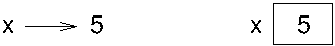
\includegraphics[width=2.5in]{figs/variables.pdf}}
%\caption{Diagrams that represent variables in Python (left) and
%C (right).}
%\label{variables}
%\end{figure}


%\section{The compilation process}
\section{编译流程}
%As a programmer, you should have a mental model of what happens
%during compilation.  If you understand the process, it will help
%you interpret error messages, debug your code, and avoid
%common pitfalls.
作为程序员, 你应该对编译期间发生了什么有个大致脉络.
如果你熟悉这个过程, 便可以帮你了解错误信息, 调试代码, 
以及避免常见的陷阱.

%The steps of compilation are:
编译步骤如下:

\begin{enumerate}
%\item Preprocessing: C is one of several languages that include
%{\bf preprocessing directives} that take effect before the program is
%compiled.  For example, the \verb"#include" directive causes the
%source code from another file to be inserted at the location of the
%directive.
\item 预处理: C 是一种包括 {\bf 预处理指令} 的语言, 
  这些指令是在编译之前起效的. 比如, \verb"#include" 指令会
  将另一个文件的源代码插入到指令的位置.

%\item Parsing: During parsing, the compiler reads the source code and
%builds an internal representation of the program, called an
%{\bf abstract syntax tree}.  Errors
%detected during this step are generally syntax errors.
\item 解析: 解析期间, 编译器会读取源码并构建程序的内在结构, 也
  就是{\bf 抽象语法树}. 在此期间检查出来的错误, 通常是语法错误.

%\item Static checking: The compiler checks whether variables and
%values have the right type, whether functions are called with the
%right number and type of arguments, etc.  Errors detected during
%this step are sometimes called {\bf static semantic} errors.
\item 静态检查: 编译器会检查变量和值的类型是否正确, 
  调用函数是否使用了正确数量和类型的参数, 等等.
  此阶段侦测到的错误通常是 {\bf 静态语义} 错误.

%\item Code generation: The compiler reads the internal representation
%of the program and generates machine code or byte code.
\item 代码生成: 编译器会读取程序的内在结构, 
  并生成机器码或字节码.

%\item Linking: If the program uses values and functions defined in a
%library, the compiler has to find the appropriate library and
%include the required code.
\item 链接: 如果程序使用了库中定义的值和函数, 
  编译器需要找到合适的库, 并囊括所需的代码.

%\item Optimization: At several points in the process, the compiler
%can transform the program to generate code that runs faster or
%uses less space.  Most optimizations are simple changes that eliminate
%obvious waste, but some compilers perform sophisticated analyses and
%transformations.
\item 优化: 在整个流程的各个阶段, 编译器可以转换程序, 生成
  运行更快, 或更加节约空间的代码. 大部分的优化是一些简单的修改, 可以消除
  明显的耗费, 但有些编译器可以执行更复杂的分析和代码转换.

\end{enumerate}
%Normally when you run {\tt gcc}, it runs all of these steps and
%generates an executable file.  For example, here is a minimal C
%program:
通常运行{\tt gcc}时, 它会执行所有这些步骤, 生成一个可执行文件.
比如, 下面是一个极简的C程序代码:

\begin{verbatim}
#include <stdio.h>
int main()
{
    printf("Hello World\n");
}
\end{verbatim}
%If you save this code in a file called
%{\tt hello.c}, you can compile and run it like this:
如果你将上述代码保存为一个名为{\tt hello.c}的文件, 
你便能像这样对其进行编译和执行:

\begin{verbatim}
$ gcc hello.c
$ ./a.out
\end{verbatim}

%By default, {\tt gcc} stores the executable code in a file
%called {\tt a.out} (which originally stood for ``assembler output'').
%The second line runs the executable.  The prefix \verb"./" tells
%the shell to look for it in the current directory.
默认情况下, {\tt gcc} 将可执行代码存储在名为 {\tt a.out}
(起初表示``assembler output'')的文件中.
第二行会运行可执行文件. 
前缀 \verb"./"是告诉shell在当前目录中查找.

%It is usually a good idea to use the {\tt -o} flag to provide a
%better name for the executable:
通常最好使用{\tt -o} 标识为可执行文件提供一个合适的名称:

\begin{verbatim}
$ gcc hello.c -o hello
$ ./hello
\end{verbatim}

%\section{Object code}
\section{目标码}
%The {\tt -c} flag tells {\tt gcc} to compile the program and
%generate machine code, but not to link it or generate an executable:

使用{\tt -c}标识, 可以令{\tt gcc}编译程序并生成机器码, 但并不会链接库中函数, 也就不会生成可执行文件:

\begin{verbatim}
$ gcc hello.c -c
\end{verbatim}

%The result is a file named {\tt hello.o}, where the {\tt o} stands for
%{\bf object code}, which is the compiled program.  Object code is not
%executable, but it can be linked into an executable.
结果是一个名为{\tt hello.o}的文件, 其中{\tt o}表示
{\bf 目标码}, 也就是编译后的程序. 
目标码不可执行, 但可以链接到可执行文件中.

%The UNIX command {\tt nm} reads an object file and generates
%information about the names it defines and uses.  For example:
UNIX 命令{\tt nm} 可以读取目标文件, 并生成涉及其所定义和应用的
名称的信息. 例如:

\begin{verbatim}
$ nm hello.o
0000000000000000 T main
                 U puts
\end{verbatim}
%This output indicates that {\tt hello.o} defines the name {\tt main}
%and uses a function named {\tt puts}, which stands for ``put string''.
%In this example, {\tt gcc} performs an optimization by replacing
%{\tt printf}, which is a large and complicated function, with
%{\tt puts}, which is relatively simple.
输出结果表明{\tt hello.o}定义了名称{\tt main}, 以及名
为{\tt puts}的函数, 这个名字表示``put string''.
在这个例子中, {\tt gcc} 通过将庞大复杂的{\tt printf}函数,
替换为相对简单的{\tt puts}, 以进行优化.


%You can control how much optimization {\tt gcc} does with
%the {\tt -O} flag.  By default, it does very little optimization, which
%can make debugging easier.  The option {\tt -O1} turns on the most
%common and safe optimizations.  Higher numbers turn on additional
%optimizations that require longer compilation time.
你可以使用{\tt -O}标识来控制{\tt gcc}进行多大程度的优化.
默认情况下, 它优化得很少, 这会令调试相对简单.
而选项{\tt -O1}会开启常用且安全得优化.
更高得数字会开启更多得优化, 而这也就会需要更长得编译时间.


%In theory, optimization should not change the behavior of the program,
%other than to speed it up.  But if your program has a subtle bug,
%you might find that optimization makes the bug appear or disappear.
%It is usually a good idea to turn off optimization while you are developing
%new code.  Once the program is working and passing appropriate tests,
%you can turn on optimization and confirm that the tests still pass.
理论上, 优化除了加速程序之外, 不应该改变程序的行为. 
但如果你的程序存在微妙的错误, 那你可能会发现, 优化会令错误暴露
或消失. 通常在开发新代码时, 最好关闭优化.
一旦程序正常运行, 并能通过适当的测试, 你便可以
开启优化, 并确认测试仍然通过.

%\section{Assembly code}
\section{汇编码}

%Similar to the {\tt -c} flag, the {\tt -S} flag tells {\tt gcc}
%to compile the program and generate assembly code, which is basically
%a human-readable form of machine code.

类似于{\tt -c}标识, {\tt -S} 标识会令{\tt gcc}编译程序并生成
汇编码, 而这基本上是一种人可读的机器码形式.

\begin{verbatim}
$ gcc hello.c -S
\end{verbatim}
%The result is a file named {\tt hello.s}, which might look something like
%this:
结果是一个名为{\tt hello.s}的文件, 看起来像这样:

\begin{verbatim}
        .file        "hello.c"
        .section     .rodata
.LC0:
        .string      "Hello World"
        .text
        .globl       main
        .type        main, @function
main:
.LFB0:
        .cfi_startproc
        pushq %rbp
        .cfi_def_cfa_offset 16
        .cfi_offset 6, -16
        movq %rsp, %rbp
        .cfi_def_cfa_register 6
        movl $.LC0, %edi
        call puts
        movl $0, %eax
        popq %rbp
        .cfi_def_cfa 7, 8
        ret
        .cfi_endproc
.LFE0:
        .size        main, .-main
        .ident       "GCC: (Ubuntu/Linaro 4.7.3-1ubuntu1) 4.7.3"
        .section     .note.GNU-stack,"",@progbits
\end{verbatim}
%{\tt gcc} is usually configured to generate code for the machine you
%are running on, so for me it generates x86 assembly language,
%which runs on a wide variety of processors from Intel, AMD, and
%others.  If you are running on a different architecture, you might
%see different code.

{\tt gcc} 通常会被设置, 为你运行的机器生成相应的代码,
所以对我来说, 它会生成x86汇编语言,
这可以在Intel, AMD 和其他厂商的多种处理器上运行.
如果你在不同架构上运行, 你可能会得到不同的代码.

%\section{Preprocessing}
\section{预处理}
%Taking another step backward through the compilation process, you
%can use the {\tt -E} flag to run the preprocessor only:
现在我们在编译过程中向后再走一步.
你可以用{\tt -E}标识, 仅仅只运行预处理器:

\begin{verbatim}
$ gcc hello.c -E
\end{verbatim}
%The result is the output from the preprocessor.  In this example,
%it contains the included code from {\tt stdio.h}, and all the files
%included from {\tt stdio.h}, and all the files included from those
%files, and so on.  On my machine, the total is more than 800 lines
%of code.  Since almost every C program includes {\tt stdio.h}, those
%800 lines of code get compiled a lot.  If, like many C programs,
%you also include {\tt stdlib.h}, the result is more than 1800 lines
%of code.
结果是预处理器的输出.
这个例子中, 它包含了{\tt stdio.h}中包含的代码, 
以及{\tt stdio.h}中包含的所有文件, 依此类推.
在我的机器上, 结果有800多行代码.
由于几乎每个C程序都包括{\tt stdio.h}, 所以这800行代码会被编译多次.
如果像很多C程序一样, 你也包含了{\tt stdlib.h},
那么结果要超过1800行代码了.

%\section{Understanding errors}
\section{理解错误}

%Now that we know the steps in the compilation process, it is easier
%to understand error messages.  For example, if there is an error
%in a \verb"#include" directive, you'll get a message from the
%preprocessor:
现在我们知道了编译过程的各个步骤, 
便更容易理解错误信息了.
比如, 如果\verb"#include" 指令中存在错误, 
你会从预处理器得到下面这条信息:

\begin{verbatim}
hello.c:1:20: fatal error: stdioo.h: No such file or directory
compilation terminated.
\end{verbatim}

%If there's a syntax error, you get a message from the compiler:
如果存在语法错误, 你会从编译器得到下面信息:

\begin{verbatim}
hello.c: In function 'main':
hello.c:6:1: error: expected ';' before '}' token
\end{verbatim}

%If you use a function that's not defined in any of the standard
%libraries, you get a message from the linker:
如果使用了任何标准库都没有定义的函数,
你会从链接器得到下面错误信息:

\begin{verbatim}
/tmp/cc7iAUbN.o: In function `main':
hello.c:(.text+0xf): undefined reference to `printff'
collect2: error: ld returned 1 exit status
\end{verbatim}
%{\tt ld} is the name of the UNIX linker, so named because ``loading''
%is another step in the compilation process that is closely related
%to linking.
{\tt ld}是UNIX链接器的名称, 
如此命名是因为``loading'' 是编译过程中和链接关系密切的另一步骤.


%Once the program starts, C does very little runtime checking,
%so there are only a few runtime errors you are likely to see.  If you
%divide by zero, or perform another illegal floating-point operation, you
%will get a ``Floating point exception.''  And if you try to read or
%write an incorrect location in memory, you will get a ``Segmentation
%fault.''
一旦程序运行, C 便几乎不会进行运行时检查,
所以你可能只会看到极少的运行时错误.
如果你除以零, 或者执行了其他非法的浮点操作, 
你会得到一个``Floating point exception(浮点异常).''
同时, 如果你尝试读取或写入一个错误的内存位置,
你会遇到 ``Segmentation fault(段错误).''

% TODO: -Wall and lint

%\chapter{Processes}
%
%\section{Abstraction and virtualization}
\chapter{进程}

\section{抽象和虚拟化}
%Before we talk about processes, I want to define a few words:
在我们谈论进程之前, 我想先定义几个词汇:

\begin{itemize}

%\item Abstraction: An abstraction is a simplified representation
%of something complicated.  For example, if you drive a car, you
%understand that when you turn the wheel left, the car goes left,
%and vice versa.  Of course, the steering wheel is connected to
%a sequence of mechanical and (often) hydraulic systems that turn
%the wheels, and the wheels interact with the road in ways that
%can be complex, but as a driver, you normally don't have to think
%about any of those details.  You can get along very well with
%a simple mental model of steering.  Your mental model is an
%abstraction.
\item 抽象: 抽象是某个复杂事物的简化表达.
例如, 当你开车时, 你知道当你左转方向盘时, 车会左转,
反之亦然. 当然, 方向盘连接着一系列机械和(通常是)液压系统, 
这些会使车轮转动, 同时车轮会以复杂的方式和路面互动.
作为一个司机, 你通常无需考虑这些细节. 你只需要一个
简单的逻辑模型来进行驾驶. 你的这个逻辑模型便是一种抽象.


%Similarly, when you use a web browser, you understand that when
%you click on a link, the browser displays the page the link refers
%to.  The software and network communication that make that possible
%are complex, but as a user, you don't have to know the
%details.
同样地, 当你使用网络浏览器时, 你知道当你点击链接时,
浏览器会显示该链接所指的页面.
使这一切成为可能的软件和网络通信是复杂的.
但作为一个用户, 你不必了解其细节.

%A large part of software engineering is designing abstractions like
%these that allow users and other programmers to use powerful
%and complicated systems without having to know about the details
%of their implementation.
软件工程中一个重要部分就是设计想这样的抽象,
这些抽象可以使用户和其他程序员能够使用强大而复杂的系统,
而无需了解其实现的细节.

%\item Virtualization: An important kind of abstraction is
%virtualization, which is the process of creating a desirable
%illusion.
\item 虚拟化: 一种重要的抽象便是虚拟化, 这是创建一个令人满意的幻觉的过程.


%For example, many public libraries participate in inter-library
%collaborations that allow them to borrow books from each other.
%When I request a book, sometimes the book is on the shelf at my
%local library, but other times it has to be transferred from another
%collection.  Either way, I get a notification when it is available
%for pickup.  I don't need to know where it came from, and I don't
%need to know which books my library has.  As a whole, the system
%creates the illusion that my library has every book in the world.
例如, 很多公共图书馆会参与图书馆之间的协作, 允许其相互借书.
当我请求一本图书时, 有时这本书是在我当地的图书馆的书架上,
但其他时候, 它需要从另外的地方转移过来.
无论哪种情况, 当书籍可以领取时, 我都会接到通知.
我不必知道它来自哪里, 我也不需要知道我的图书馆里有哪些书.
整个系统创建了一个假象, 让我相信我的图书馆拥有世界上的任意一本图书.


%The collection physically located at my local library might be small,
%but the collection available to me virtually includes every book
%in the inter-library collaboration.
我当地的图书馆里实际可用的书可能很少,
但对我来说, 可用的虚拟书籍包括合作的图书馆中的每一本书.

%As another example, most computers are only connected to one
%network, but that network is connected to others, and so on.  What
%we call the Internet is a collection of networks and a set of
%protocols that forward packets from one network to the next.
%From the point of view of a user or programmer, the system behaves
%as if every computer on the Internet is connected to every other
%computer.  The number of physical connections is small, but the
%number of virtual connections is very large.
再举个例子, 大多数计算机只连接到一个网络, 
但该网络会连接到其他网络, 依此类推.
我们所称的互联网是一组网络和协议, 
它们可以将数据包从一个网络转发到下一个网络. 
从用户或程序员的角度来看, 
该系统表现得好像互联网上的每台计算机都与其他计算机相连. 
所以物理连接的数量虽然很少, 但虚拟连接的数量是非常大的.

\end{itemize}

%The word ``virtual'' is often used in the context of a virtual
%machine, which is software that creates the illusion of a dedicated
%computer running a particular operating system, when in reality
%the virtual machine might be running, along with many other virtual
%machines, on a computer running a different operating system.
``虚拟''一词通常在虚拟机的上下文中使用, 虚拟机是一种软件, 会给你一种假象,
彷佛你运行在一个运行着特定操作系统的专有机器上.
而实际上, 虚拟机可能和很多其他虚拟机一起运行在同一台计算机上, 这些虚拟机可能运行着
不同的操作系统.

%In the context of virtualization, we sometimes call what is
%really happening ``physical'', and what is virtually happening
%either ``logical'' or ``abstract.''
在虚拟化的上下文中, 我们有时称真实发生的事情为``物理事件'', 
而虚拟发生的事情为``逻辑事件''或者``抽象事件''.

%\section{Isolation}
\section{隔离}

%One of the most important principles of engineering is isolation:
%when you are designing a system with multiple components, it is usually
%a good idea to isolate them from each other so that a change in one
%component doesn't have undesired effects on other components.
工程学最重要的一个原则便是隔离:
当你设计一个包括多个部件的系统时, 最好将其相互之间进行隔离,
如此一个部件的改变就不会给其他组件带来不良影响.

%One of the most important goals of an operating system is to isolate
%each running program from the others so that programmers don't have to
%think about every possible interaction.  The software object that
%provides this isolation is a {\bf process}.
操作系统的一个重要目标便是将每个运行的程序和其他程序进行隔离,
如此程序员便无需关注任何交互的可能.
提供这种隔离性的软件对象叫做{\bf 进程}.

%A process is a software object that represents a running program.
%I mean ``software object'' in the sense of object-oriented programming;
%in general, an object contains data and provides methods
%that operate on the data.  A process is an object that contains the
%following data:
进程是一个表示当前运行程序的软件对象.
我说的``软件对象''是指面向对象编程中的对象;
通常, 对象包含数据以及操作数据的方法.
一个进程便是一个包含下面数据的对象:

\begin{itemize}

%\item The text of the program, usually a sequence of
%machine language instructions.
\item 程序的文本, 通常是一系列机器语言指令.

%\item Data associated with the program, including static data (allocated
%at compile time) and dynamic data (allocated at run time).
\item 程序相关的数据, 包括静态数据(编译时分配)和动态数据(运行时分配).

%\item The state of any pending input/output operations.  For example,
%if the process is waiting for data to be read from disk or for a
%packet to arrive on a network, the status of these operations is
%part of the process.
\item 任何未完成的输入/输出操作的状态. 比如, 
  如果进程正在等待从磁盘读取数据, 或者等待网络数据到达, 
  这些操作的状态便是进程的一部分.

%\item The hardware state of the program, which includes data stored
%in registers, status information, and the program counter, which
%indicates which instruction is currently executing.
\item 程序的硬件状态, 包括寄存器中的数据, 状态信息以及程序计数器.
  程序计数器用来标识当前正在执行哪个指令.

\end{itemize}
%Usually one process runs one program, but it is also possible for
%a process to load and run a new program.
通常一个进程运行一个程序, 但也可能会加载并运行新的程序.


%It is also possible, and common, to run the same program in more than one
%process.  In that case, the processes share the same program text
%but generally have different data and hardware states.
还有可能, 也是很常见的情况是, 
多个进程中运行同一个程序. 在这种情况下, 这些进程会共享相同的程序代码,
但通常数据和硬件状态不同.

%Most operating systems provide a fundamental set of capabilities
%to isolate processes from each other:
多数操作系统会提供一组基础功能, 以使进程之间相互隔离:

\begin{itemize}

%\item Multitasking: Most operating systems have the ability to
%interrupt a running process at almost any time, save its hardware
%state, and then resume the process later.  In general, programmers
%don't have to think about these interruptions.  The program behaves
%as if it is running continuously on a dedicated processor, 
%except that the time between instructions is unpredictable.
\item 多任务: 多数操作系统都具有一种能力,
  可以在任何时刻将运行中的进程中断, 并保存其硬件状态,
  然后稍后恢复进程.
  通常, 程序员不必考虑这些中断.
  程序的行为就像在专用处理器上连续运行一样,
  只是指令之间的时间是不可预测的.


%\item Virtual memory: Most operating systems create the
%illusion that each process has its own chunk of memory, isolated
%from all other processes.  Again, programmers generally don't
%have to think about how virtual memory works; they can proceed
%as if every program has a dedicated chunk of memory.
\item 虚拟内存: 多数操作系统都会创建这样的假象, 
  即每个进程都有自己的一段空间, 与其他进程都隔离开来.
  同样地, 程序员一般无需关注虚拟内存如何工作; 
  他们可以按照每个程序都有一段专门的内存来进行操作.


%\item Device abstraction: Processes running on the same computer share
%the disk drive, the network interface, the graphics card, and other
%hardware.  If processes interacted with this hardware directly,
%without coordination, chaos would ensue.  For example, network data
%intended for one process might be read by another.  Or multiple
%processes might try to store data in the same location on a hard
%drive.  It is up to the operating system to maintain order by
%providing appropriate abstractions.
\item 设备抽象: 运行在同一个计算机上的进程, 共享磁盘驱动器, 网络接口, 
  图形卡, 以及其他硬件. 如果进程不经协商便直接和硬件交互, 便会引发混乱.
  例如, 本来要传递给某个进程的网络数据, 可能被其他进程读取, 
  或多个进程向硬盘上同一个位置存储数据.
  这便有赖于操作系统提供适当的抽象, 以维护秩序.

\end{itemize}
%As a programmer, you don't need to know much about how these
%capabilities are implemented.  But if you are
%curious, you will find a lot of interesting things
%going on under the metaphorical hood.  And if you know what's
%going on, it can make you a better programmer.
作为程序员, 你并不需要知道这些功能实现的详情.
但如果你有兴趣, 你会发现在各种隐喻之下, 
有很多有趣的事情正在发生.
如果你知晓发生的细节, 那你将成为更好的程序员.

%\section{UNIX processes}
\section{UNIX 进程}
\label{unixps}
%While I write this book, the process I
%am most aware of is my text editor, emacs.  Every once in a while
%I switch to a terminal window, which is a window running a UNIX shell
%that provides a command-line interface.
当写这本书时, 我最关注的进程是我的文本编辑器, emacs.
每隔一段时间, 我会切换到终端窗口.
这是一个运行 UNIX shell 的窗口, 它提供了命令行界面.

%When I move the mouse, the window manager wakes up, sees that the
%mouse is over the terminal window, and wakes up the terminal.
%The terminal wakes up the shell.
%If I type {\tt make} in the shell, it creates a
%new process to run Make, which creates another process to run LaTeX
%and then another process to display the results.
当我移动鼠标, 窗口管理器便会被唤醒, 查看鼠标是否在终端窗口上,
然后又会唤醒终端. 终端唤醒shell. 
如果我在shell中输入{\tt make}, 
它会创建一个新的进程来执行 Make, 创建另一个进程运行 LaTeX,
然后再创建一个进程来显示结果.

%If I need to look something up, I might switch to another desktop,
%which wakes up the window manager again.  If I click on the icon for a
%web browser, the window manager creates a process to run the web
%browser.  Some browsers, like Chrome, create a new process for each
%window and each tab.
如果我需要查找一些东西, 我可能会切换到另一个桌面,
这也会再次唤醒窗口管理器.
如果我点击网络浏览器的图标, 窗口管理器会创建一个进程, 运行网络浏览器.
有些浏览器, 比如 Chrome, 会为每个窗口和每个标签页都创建新的进程.

%And those are just the processes I am aware of.  At the same time
%there are many other processes running in the {\bf background}.
%Many of them are performing operations related to the operating
%system.
这些还只是我知道的进程.
同时, 还有很多其他进程在{\bf 后台} 运行.
其中很多进程正在执行与操作系统相关的操作.

%The UNIX command {\tt ps} prints information about running processes.
%If you run it in a terminal, you might see something like this:
UNIX 命令 {\tt ps} 可以打印正在运行的进程的信息.
如果你在终端执行它, 你可能会看到像这样的东西:

\begin{verbatim}
  PID TTY          TIME CMD
 2687 pts/1    00:00:00 bash
 2801 pts/1    00:01:24 emacs
24762 pts/1    00:00:00 ps
\end{verbatim}
%The first column is the unique numerical process ID.  The second
%column is the terminal that created the process; 
%``TTY'' stands for teletypewriter, which was the original
%mechanical terminal.
%
%The third column is the total processor time used by the process,
%in hours, minutes, and seconds.
%The last column is the name of the running program.  In
%this example, {\tt bash} is the name of the shell that interprets
%the commands I type in the terminal, emacs is my text editor, and
%ps is the program generating this output.

第一列是唯一的数字格式进程ID.
第二列是创建进程的终端; 
``TTY''代表电传打印机, 这是最早的机械终端.

第三列是进程使用的处理器总时间, 以小时、分钟和秒为单位.
在这个例子中, {\tt bash} 是解释输入命令的 shell 的名称,
emacs 是我的文本编辑器, ps 是生成此输出的程序.

%By default, {\tt ps} lists only the processes associated with
%the current terminal.  If you use the {\tt -e} flag, you get every
%process (including processes belonging to other users, which is
%a security flaw, in my opinion).
%
%On my system there are currently 233 processes.
%Here are some of them:
默认情况下, {\tt ps} 仅列出和当前终端相关的进程.
如果你使用{\tt -e} 标志, 你便能获取每个进程(包括属于其他用户的进程,
就我看来, 这是一个安全漏洞).

在我的系统上, 目前有233个进程.
下面是其中一些:

\begin{verbatim}
  PID TTY          TIME CMD
    1 ?        00:00:17 init
    2 ?        00:00:00 kthreadd
    3 ?        00:00:02 ksoftirqd/0
    4 ?        00:00:00 kworker/0:0
    8 ?        00:00:00 migration/0
    9 ?        00:00:00 rcu_bh
   10 ?        00:00:16 rcu_sched
   47 ?        00:00:00 cpuset
   48 ?        00:00:00 khelper
   49 ?        00:00:00 kdevtmpfs
   50 ?        00:00:00 netns
   51 ?        00:00:00 bdi-default
   52 ?        00:00:00 kintegrityd
   53 ?        00:00:00 kblockd
   54 ?        00:00:00 ata_sff
   55 ?        00:00:00 khubd
   56 ?        00:00:00 md
   57 ?        00:00:00 devfreq_wq
\end{verbatim}

%{\tt init} is the first process created when the operating system
%starts.  It creates many of the other processes, and then sits idle
%until the processes it created are done.
{\tt init} 是操作系统启动时创建的第一个进程.
它会创建许多其他进程, 然后闲置, 
直到它创建的进程都结束.


%{\tt kthreadd} is a process the operating system uses to create new
%{\bf threads}.  We'll talk more about threads later, but for now you can
%think of a thread as kind of a process.  The {\tt k} at the beginning
%stands for {\bf kernel}, which is the part of the operating system
%responsible for core capabilities like creating threads.  The extra
%{\tt d} at the end stands for {\bf daemon}, which is another name for
%processes like this that run in the background and provide operating
%system services.  In this context, ``daemon'' is used in the
%sense of a helpful spirit, with no connotation of evil.
{\tt kthreadd} 是操作系统用来创建 {\bf 线程} 的进程.
后续我们将更详细地讨论线程, 当前你可以将线程看作是一种进程.
开头的{\tt k} 代表 {\bf 内核(kernel)},
这是操作系统符合核心功能(比如创建线程)的部分.
结尾的 {\tt d} 代表 {\bf 守护程序(daemon)},
这是运行在后台, 并提供操作系统服务的进程的另一个名称.
在此, ``daemon'' 是指一种乐于助人的精神, 没有任何邪恶的意思.
 
% Based on the name, you can infer that {\tt ksoftirqd} is also a kernel
% daemon; specifically, it handles software interrupt requests, or
% ``soft IRQ''.
根据名称, 你可以推断出{\tt ksoftirqd} 也是一个内核守护程序;
具体来说, 它处理软件中断请求, 即 ``软中断(soft IRQ)''

%{\tt kworker} is a worker process created by the kernel to do some
%kind of processing for the kernel.
{\tt kworker} 是一个内核创建的工作进程, 用来为内核处理一些任务.

%There are often multiple processes running these kernel services.
%On my system at the moment, there are 8 {\tt ksoftirqd} processes
%and 35 {\tt kworker} processes.
通常有多个进程运行着内核服务.
在我的系统上, 现在有8个{\tt ksoftirqd} 进程和35个{\tt kworker} 进程.

%I won't go into more details about the other processes, but if you
%are interested you can search for more information about them.
%You should run {\tt ps} on your system and compare your results
%to mine.
我不会详细讨论其他进程, 但如果你感兴趣, 
你可以搜索更多关于它们的信息.
你应该在你的系统上运行 {\tt ps}, 并将结果和我的进行对比.

%TODO: using gdb here?

%\chapter{Virtual memory}
%
%\section{A bit of information theory}
\chapter{虚拟内存}

\section{一点信息论知识}

%A {\bf bit} is a binary digit; it is also a unit of information.  If you
%have one bit, you can specify one of two possibilities, usually
%written 0 and 1.  If you have two bits, there are 4 possible
%combinations, 00, 01, 10, and 11.  In general, if you have $b$ bits, you
%can indicate one of $2^b$ values.  A {\bf byte} is 8 bits, so it can
%hold one of 256 values.
%
%Going in the other direction, suppose you want to store a letter
%of the alphabet.  There are 26 letters, so how many bits do you
%need?  With 4 bits, you can specify one of 16 values, so that's
%not enough.  With 5 bits, you can specify up to 32 values, so
%that's enough for all the letters, with a few values left over.

{\bf 比特(bit)} 是一个二进制的数位, 也是一个信息单元.
如果你有一比特, 便可以表示两种可能性中的一种, 通常写作 0 和 1.
如果你有两比特, 那边有4种组合, 分别是 00, 01, 10, 和 11.
通常, 如果你有 $b$ 个比特, 你便可以表示 $2^b$个值.
一个{\bf 字节(byte)} 是8个比特, 所以可以表示256个值.

反过来想, 假设你想储存一个字母. 字母表有26个字母, 
那么你需要几个比特呢? 如果用4个比特, 你可以表示16个值, 数量不够.
如果用5个比特, 你可以表示多达32个值, 这足够表示所有字母了, 而且还有剩余.

%In general, if you want to specify one of $N$ values, you should
%choose the smallest value of $b$ so that $2^b \ge N$.  Taking the
%log base 2 of both sides yields $b \ge log_2 N$.
%
%Suppose I flip a coin and tell you the outcome.  I have given
%you one bit of information.  If I roll a six-sided die and tell
%you the outcome, I have given you $log_2 6$ bits of information.
%And in general, if the probability of the outcome is 1 in $N$,
%then the outcome contains $log_2 N$ bits of information.

通常, 如果你想表示$N$个值, 你应该选择满足 $2^b \ge N$ 的最小 $b$ 值.
两侧以2为底取对数, 便可以得到 $b \ge log_2 N$.

假设我掷一枚硬币, 并告诉你结果, 那么我便是给了你一比特的信息.
如果我掷一个六面骰子, 并告诉你结果, 那我便是给了你 $log_2 6$ 个比特的信息.
通常, 如果发生的概率是$N$中的1个, 那么结果便包含 $log_2 N$ 个比特信息.

%Equivalently, if the probability of the outcome is $p$, then
%the information content is $-log_2 p$.  This quantity is called
%the {\bf self-information} of the outcome.  It measures
%how surprising the outcome is, which is why it is also called
%{\bf surprisal}.  If your horse has only one chance in 16 of winning,
%and he wins, you get 4 bits of information (along with the
%payout).  But if the favorite wins 75\% of the time, the news
%of the win contains only 0.42 bits.
%
%Intuitively, unexpected news carries a lot of
%information; conversely, if there is something you were already confident
%of, confirming it contributes only a small amount of information.
%
%For several topics in this book, we will need to be comfortable
%converting back and forth between the number of bits, $b$, and the
%number of values they can encode, $N = 2^b$.
同样的, 如果结果出现的概率是 $p$, 那么信息量便是 $-log_2 p$.
这个数量也被称为结果的{\bf 自信息}, 它是用来衡量结果的惊奇程度, 
所以也被称为{\bf 惊奇度}. 如果你的马仅有$1/16$的概率获胜,
但是赢了, 你可以4比特的信息(以及赔付). 
但如果获胜的机率是75\%, 那么胜利的消息只包含0.42比特.

直观来说, 出乎意料的消息反而包含了大量的信息.
相反, 如果你已经确定某件事情, 那么证实它仅会提供少量信息.

在本书的诸多主题中, 我们需要在比特数, $b$, 和其能编码的值的数量 $N = 2^b$ 之间
熟练转换.

%\section{Memory and storage}
\section{内存和存储}
%While a process is running, most of its data is held in {\bf main
%	memory}, which is usually some kind of random access memory (RAM).
%On most current computers, main memory is {\bf volatile}, which means that
%when the computer shuts down, the contents of main memory are lost.
%A typical desktop computer has 2--8 GiB of
%memory.  GiB stands for ``gibibyte,'' which is $2^{30}$ bytes.  
%
%If the process reads and writes files, those files are usually stored
%on a hard disk drive (HDD) or solid state drive (SSD).  These storage
%devices are {\bf non-volatile}, so they are used for long-term storage.
%Currently a typical desktop computer has a HDD with a capacity of 500
%GB to 2 TB.  GB stands for ``gigabyte,'' which is $10^9$ bytes.  TB
%stands for ``terabyte,'' which is $10^{12}$ bytes.

进程运行时, 其大部分数据存储在{\bf 主内存}, 这通常是一种随机访问存储(RAM).
当前多数计算机上, 主存储都是{\bf 易失的}, 也就意味着一旦计算机关机, 
主存储的内容便会丢失. 一台典型的桌面计算机有 2--8 GiB 内存.
GiB 表示``gibibyte,'' 也就是 $2^{30}$ 字节.

进程需要读写文件, 而文件往往存储在硬盘驱动器(HDD)或者固态硬盘中.
这些存储设备都是 {\bf 非易失的}, 因此可以用作长期存储.
目前一台典型桌面计算机会拥有500GB到2TB容量的硬盘.
其中GB表示``gigabyte,'' 也就是 $10^9$ 字节.
TB 表示 ``terabyte,'' 也就是 $10^{12}$ 字节.

%You might have noticed that I used the binary unit
%GiB for the size of main memory and the decimal units GB and TB for
%the size of the HDD.  For historical and technical reasons, memory is
%measured in binary units, and disk drives are measured in decimal
%units.  In this book I will be careful to distinguish binary and
%decimal units, but you should be aware that the word ``gigabyte'' and the
%abbreviation GB are often used ambiguously.
%
%In casual use, the term ``memory'' is sometimes used for HDDs and SSDs
%as well as RAM, but the properties of these devices are very
%different, so we will need to distinguish them.  I will use
%{\bf storage} to refer to HDDs and SSDs.
你可能已经注意到, 我描述主内存大小时, 用二进制单位GiB,
描述硬盘大小时, 用十进制单位GB和TB.
由于一些历史和科技的原因, 内存通常用二进制单位衡量, 而硬盘则用十进制单位.
在本书中, 我将谨慎区分二进制和十进制单位,
但你也应该注意到, ``gigabyte''和缩写GB通常是混用的.
%TODO:gibabyte 不是等于GB吗,还是想表达 gibibyte 和GB?

在非正式的使用中, ``内存''一词有时候会指 HDD和SSD, 以及 RAM. 但
这些设备的属性是不同的, 所以我们需要仔细区分它们. 我将使用
{\bf 存储} 来指代 HDD和SSD.

%\section{Address spaces}
\section{地址空间}
%Each byte in main memory is specified by an integer {\bf physical
%	address}.  The set of valid physical addresses is called the
%physical {\bf address space}.  It
%usually runs from 0 to $N-1$, where $N$ is
%the size of main memory.  On a system with 1 GiB of physical memory,
%the highest valid address is $2^{30}-1$, which is 1,073,741,823 in
%decimal, or 0x3fff ffff in hexadecimal (the prefix 0x indicates a
%hexadecimal number).
%
%However, most operating systems provide {\bf virtual memory}, which
%means that programs never deal with physical addresses, and don't 
%have to know how much physical memory is available.

主内存中的每个字节都由一个整数{\bf 物理地址}指定.
有效的物理地址集被称为物理{\bf 地址空间}.
通常从0 到 $N-1$, 其中$N$ 是内存的大小.
在1 GiB 物理内存的系统上, 最高的有效地址是$2^{30}-1$, 
即十进制下的1,073,741,823 , 或者十六进制下的0x3fff ffff(前缀的 0x 表示十六进制数).

然而, 大部分的操作系统会提供{\bf 虚拟内存}, 这意味着程序永远不必处理
物理地址, 也不必知道由多少物理地址可用.

%Instead, programs work with {\bf virtual addresses}, which are numbered
%from 0 to $M-1$, where $M$ is the number of valid virtual addresses.
%The size of the virtual address space is determined by the operating
%system and the hardware it runs on.
%
%You have probably heard people talk about 32-bit and 64-bit systems.
%These terms indicate the size of the registers, which is usually also
%the size of a virtual address.  On a 32-bit system, virtual addresses
%are 32 bits, which means that the virtual address space runs from 0 to
%0xffff ffff.  The size of this address space is $2^{32}$ bytes, or 4
%GiB.

相反, 程序会使用从 0 到 $M-1$ 编号的{\bf 虚拟地址}, 其中$M$ 是有效
虚拟地址的数量. 虚拟地址空间的大小是由操作系统和其运行的硬件共同决定的.

你可能听过别人谈论32位系统和64位系统.
这些术语表示的是寄存器的大小, 通常也是虚拟地址的大小.
在32位系统上, 虚拟地址为32比特, 也就是虚拟地址空间从0到0xffff ffff.
所以地址空间的大小为$2^{32}$字节, 或 4 GiB.

%On a 64-bit system, the size of the virtual address space is $2^{64}$
%bytes, or $2^4 \cdot 1024^6$ bytes.  That's 16 exbibytes, which is
%about a billion times bigger than current physical memories.  It might
%seem strange that a virtual address space can be so much bigger
%than physical memory, but we will see soon how that works.
%
%When a program reads and writes values in memory, it generates virtual
%addresses.  The hardware, with help from the operating system,
%translates to physical addresses before accessing main memory.  This
%translation is done on a per-process basis, so even if two processes
%generate the same virtual address, they would map to different
%locations in physical memory.
%
%Thus, virtual memory is one important way the operating system
%isolates processes from each other.  In general, a process cannot
%access data belonging to another process, because there is no
%virtual address it can generate that maps to physical memory
%allocated to another process.
而在64位系统上, 虚拟地址空间是$2^{64}$字节, 或$2^4 \cdot 1024^6$ 字节.
这是16 艾字节, 约为当前物理内存的十亿倍.
虚拟地址空间比物理内存大这么多, 这看起来很奇怪, 
但是我们稍后就会看到它是如何工作的.

当程序从内存读取或者向内存写入值时, 它会生成虚拟地址.
在操作系统的帮助下, 访问内存之前, 硬件会被转换成物理地址.
这种转换是基于每个进程进行的, 所以即使两个进程生成同样的虚拟地址,
它们也会映射到物理内存的不同位置.

最后, 虚拟内存是操作系统隔离进程的一种重要手段.
通常, 一个进程是无法访问另一个进程拥有的数据的, 
因为如果某块物理内存已经被分配给了其他进程,
那么该进程便无法生成映射到这块物理内存的虚拟地址.

%\section{Memory segments}
\section{内存段}

%The data of a running process is organized into five segments:
运行中得进程的数据会被组织成五个段:

\begin{itemize}

%\item The {\bf code segment} contains the program text; that is, the
%machine language instructions that make up the program.
\item {\bf 代码段} 包含程序文本; 也就是构成程序的机器语言指令.

%\item The {\bf static segment} contains immutable values, like string
%literals.  For example, if your program contains the string
%{\tt "Hello, World"}, those characters will be stored in the
%static segment.
\item {\bf 静态段} 包含不可变的值, 像字符串常量. 比如, 如果你的程序包含
字符串{\tt "Hello, World"}, 那这些字符会被保存在静态段.


%\item The {\bf global segment} contains global variables and local variables that are declared {\tt static}.
\item {\bf 全局段} 包含全局变量和被声明为{\bf static(静态类型)}的
局部变量.

%\item The {\bf heap segment} contains chunks of memory allocated
%at run time, most often by calling the C library function
%{\tt malloc}.
\item {\bf 堆段} 包含运行时被分配的内存块, 通常是通过调用C库函数
{\bf malloc}所分配.

%\item The {\bf stack segment} contains the call stack, which is a
%sequence of stack frames.  Each time a function is called, a stack
%frame is allocated to contain the 
%parameters and local variables of the function.  When the function
%completes, its stack frame is removed from the stack.
\item {\bf 栈段} 包含调用栈, 也就是一系列的堆栈帧.
每次函数被调用, 都会为其分配一个包含函数的参数和局部变量的堆栈帧.
当函数运行结束, 其堆栈帧会从栈中移除. 

\end{itemize}

%The arrangement of these segments is determined partly by the 
%compiler and partly by the operating system.  The details vary
%from one system to another, but in the most common arrangement:
段的排序部分由编译器决定, 部分由操作系统决定.
具体细节取决于操作系统, 但常见的排列方式包括::

\begin{itemize}
%\item The text segment is near the ``bottom'' of memory, that is,
%at addresses near 0.
%
%\item The static segment is often just above the text segment, that is,
%at higher addresses.
%
%\item The global segment is often just above the static segment.
%
%\item The heap is often above the global segment.  As it expands,
%it grows up toward larger addresses.
%
%\item The stack is near the top of memory; that is, near the
%highest addresses in the virtual address space.  As the
%stack expands, it grows down toward smaller addresses.
\item 文本段位于内存接近``底部''的位置, 也就是靠近地址0的地方.

\item 静态段通常在文本段上方, 也就是高地址位置.

\item 全局段通常位于静态段上方.

\item 堆通常在全局段上方. 随着堆的扩张, 它会向更大地址增长.
  
\item 栈靠近内存的顶部; 也就是虚拟地址空间中最高地址附近.
栈扩展时, 会朝着更小地址方向增长.

\end{itemize}

%TODO: Figure out how to handle the code that is in both ExercisesInC
% and the repo for the book.

%To determine the layout of these segments on your system, try running
%this program, which is in {\tt aspace.c} in the repository for this
%book (see Section~\ref{code}).
若要确定你系统上这些段的布局, 尝试运行这个程序,在本书仓库
中的 {\tt aspace.c} 文件中(详见第~\ref{code}节). 


\begin{verbatim}
#include <stdio.h>
#include <stdlib.h>

int global;

int main ()
{
    int local = 5;
    void *p = malloc(128);
    char *s = "Hello, World";

    printf ("Address of main is %p\n", main);
    printf ("Address of global is %p\n", &global);
    printf ("Address of local is %p\n", &local);
    printf ("p points to %p\n", p);
    printf ("s points to %p\n", s);
}
\end{verbatim}

%{\tt main} is the name of a function; when it is used as a variable,
%it refers to the address of the first machine language instruction
%in {\tt main}, which we expect to be in the text segment.
%
%{\tt global} is a global variable, so we expect it to be in the
%global segment.  {\tt local} is a local variable, so we expect it
%to be on the stack.
%
%{\tt s} refers to a ``string literal", which is a string that appears
%as part of the program (as opposed to a string that is read from a file,
%input by a user, etc.).  We expect the location of the string to be
%in the static segment (as opposed to the pointer, {\tt s}, which is
%a local variable).
%
%{\tt p} contains an address returned by {\tt malloc}, which allocates
%space in the heap.  ``malloc'' stands for ``memory allocate.''
%
%The format sequence \verb"%p" tells {\tt printf} to format each
%address as a ``pointer'', so it displays the results in hexadecimal.
%
%When I run this program, the output looks like this (I added spaces
%to make it easier to read):
{\tt main}是这个函数的名称; 当作为变量使用时, 
它指的是{\tt main}中的第一条机器语言指令的地址, 
同时我们希望它在文本段中.

{\tt global} 是全局变量, 所以我们希望它在全局段中. 
{\tt local} 是局部变量, 我们期望它存在于栈中.

{\tt s} 指向``字符串文本'', 它是程序的一部分(与从文件读取, 
或用户输入的字符串等不同). 我们希望字符串的位置在静态段中(与指针
{\tt s}不同, 它是局部变量).

{\tt p} 包含{\tt malloc}返回的地址, 
这个函数会在堆中分配空间. ``malloc'' 表示 ``memory allocate(内存分配)''.

格式序列\verb"%p" 会告诉{\tt printf}将每个地址格式化为``指针'',
因此它会以十六进制显示结果.

当我运行这个程序, 输出如下(我增加了些空格,以便于阅读):


\begin{verbatim}
Address of main is   0x      40057d
Address of global is 0x      60104c
Address of local is  0x7ffe6085443c
p points to          0x     16c3010
s points to          0x      4006a4

\end{verbatim}
%As expected, the address of {\tt main} is the lowest, followed by
%the location of the string literal.  The location of
%{\tt global} is next, then the address {\tt p} points to.
%The address of {\tt local} is much bigger.
%
%The largest address has 12 hexadecimal digits.  Each hex digit
%corresponds to 4 bits, so it is a 48-bit address.  That suggests
%that the usable part of the virtual address space is $2^{48}$ bytes.
%
%As an exercise, run this program on your computer and compare your
%results to mine.  Add a second call to {\tt malloc} and check whether
%the heap on your system grows up (toward larger addresses).  Add a
%function that prints the address of a local variable, and check
%whether the stack grows down.
和预计的一样, {\tt main} 的地址是最低的, 然后是字符串文本的位置.
接着是{\tt global}的位置, 再然后是{\tt p}指向的地址.
{\tt local}的地址要大得多.

最大的地址有12位十六进制数. 每个十六进制数对应4个比特,
所以一共是48比特地址. 这便表示可用虚拟地址空间的大小为$2^{48}$字节.

做个练习, 在你电脑上运行这个程序, 并和我的结果进行比较.
再添加一个 {\tt malloc}, 检查你系统上的堆是否向上增长了(向更大地址方向).
再添加一个输出局部变量地址的函数, 并检查栈是否向下变化了.

%\section{Static local variables}
\section{静态局部变量}
%Local variables on the stack are sometimes called {\bf automatic},
%because they are allocated automatically when a function is called,
%and freed automatically when the function returns.
%
%In C there is another kind of local variable, called {\bf static},
%which is allocated in the global segment.  It is initialized when
%the program starts and keeps its value from one function call to
%the next.
%
%For example, the following function keeps track of how many times
%it has been called.
栈上的局部变量有时被称为{\bf 自动变量},
因为它们会在函数调用时, 自动分配, 在函数返回时, 自动释放.

在C语言中, 存在另一种局部变量, 会在全局段中进行分配, 称为{\bf 静态变量},
它会在程序启动时被初始化, 同时在函数调用之间保持其值不变.

例如, 下面的函数会跟踪其被调用的次数.

\begin{verbatim}
int times_called()
{
    static int counter = 0;
    counter++;
    return counter;
}
\end{verbatim}
%The keyword {\tt static} indicates that {\tt counter} is a static
%local variable.  The initialization happens only once, when the program
%starts.
%
%If you add this function to {\tt aspace.c} you can confirm that
%{\tt counter} is allocated in the global segment along with global
%variables, not in the stack.
关键字{\tt static}表示 {\tt counter} 是一个静态局部变量.
初始化仅会在程序启动时, 发生一次.

如果你将此函数添加到{\tt aspace.c}中, 你便可以确认{\tt counter}是在全局段中
与全局变量一起分配的, 而不是在栈中分配的.
% If you add this function to {\tt aspace.c} you can confirm that
% need a full point. 需要一个句号


%\section{Address translation}
\section{地址转换}
\label{address_translation}
%How does a virtual address (VA) get translated to a physical address (PA)?
%The basic mechanism is simple, but a simple
%implementation would be too slow and take too much space.  So actual
%implementations are a bit more complicated.

虚拟地址(VA) 如何能转换成物理地址(PA)?
基本机制很简单, 但简单的实现会太慢, 并消耗太多空间.
所以实际的实现有点复杂.

\begin{figure}
\centerline{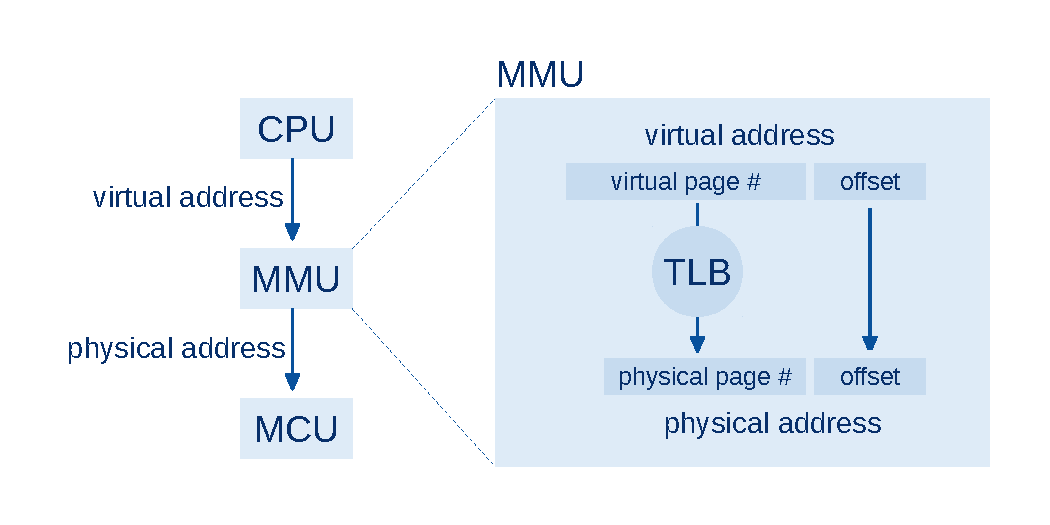
\includegraphics[width=3in]{figs/address_translation.pdf}}
\caption{地址转换过程示意图.}
%\caption{Diagram of the address translation process.}
\label{addtrans}
\end{figure}
%Most processors provide a memory management unit (MMU) that sits between the CPU and main memory.  The MMU performs fast translation between VAs and PAs.
大部分处理器会提供位于CPU和主存之间的内存管理单元(MMU).
MMU 会执行VA和PA之间的快速转换.

\begin{enumerate}

%\item When a program reads or writes a variable, the CPU generates a
%VA.  
%
%\item The MMU splits the VA into two parts, called the page number and
%the offset.  A ``page'' is a chunk of memory; the size of a page
%depends on the operating system and the hardware, but common sizes
%are 1--4 KiB.
%
%\item The MMU looks up the page number in the translation lookaside buffer (TLB) and gets the corresponding physical page number.  Then it combines
%the physical page number with the offset to produce a PA.
%
%\item The PA is passed to main memory, which reads or writes the given
%location.
\item 当程序读取或写入一个变量时, CPU会生成一个VA.

\item MMU 将VA 分成两部分, 分别是页号和偏移量.
``页''是内存的一个块, 页的大小取决于操作系统和硬件, 常见大小一般是 1--4 KiB.

\item MMU会从页表缓存 (TLB) 查找页号, 并获得相应的物理地址页号.
然后, 它将物理页号和偏移量结合起来, 构成PA.

\item PA 会传递给主存, 主存基于给定位置进行读写.

\end{enumerate}

%The TLB contains cached copies of data from the page table (which is stored in kernel memory).  The page table contains the mapping from virtual page numbers to physical page numbers.  Since each process has its own page table, the TLB has to make sure it only uses entries from the page table of the process that's running.
%
%Figure~\ref{addtrans} shows a diagram of this process.
%To see how it all works, suppose that the VA is 32 bits and the physical memory is 1 GiB, divided into 1 KiB pages.
TLB 包含来自页表(存储在内核内存中)数据的缓存副本.
页表包含虚拟页号到物理页号的映射. 
由于每个进程都有自己的页表, 因此TLB必需确保它只使用正在运行的进程的页表中的条目.

图~\ref{addtrans} 是这个过程的示意图.
若要明了其工作原理, 假设VA是32比特, 物理内存是 1 GiB, 并划分为了 1 KiB 的页.

\begin{itemize}

%\item Since 1 GiB is $2^{30}$ bytes and 1 KiB is $2^{10}$ bytes, there
%are $2^{20}$ physical pages, sometimes called ``frames.''
%
%\item The size of the virtual address space is $2^{32}$ B and the size
%of a page is $2^{10}$ B, so there are $2^{22}$ virtual pages.
%
%\item The size of the offset is determined by the page size.  In this
%example the page size is $2^{10}$ B, so it takes 10 bits to specify
%a byte on a page.
%
%\item If a VA is 32 bits and the offset is 10 bits, the remaining
%22 bits make up the virtual page number.
%
%\item Since there are $2^{20}$ physical pages, each physical page
%number is 20 bits.  Adding in the 10 bit offset, the resulting
%PAs are 30 bits.
\item 因为 1 GiB 是 $2^{30}$ 字节, 1 KiB 是 $2^{10}$ 字节, 
  所以有 $2^{20}$ 个物理页, 有时也称为 ``帧''.

\item 虚拟地址空间大小是 $2^{32}$ B, 单个页的大小是 $2^{10}$ B, 
  所以有 $2^{22}$ 个虚拟页.

\item 偏移量的大小由页面大小决定.  这个例子中, 页面大小是 $2^{10}$ B, 
  所以需要10比特来定位页面上的字节.

\item 如果 VA 是 32 比特, 同时偏移量是 10 比特, 剩下的22比特便构成了虚拟页号.

\item 由于有 $2^{20}$ 个物理页, 每个物理页号是20比特. 
  加上10比特的偏移量, 得到的 PA 便是 30 比特.

\end{itemize}
%So far this all seems feasible.  But let's think about how big a page
%table might have to be.  The simplest implementation of a page
%table is an array with one entry for each virtual page.
%Each entry would contain a physical page number, which is 20 bits
%in this example, plus some additional information about each
%frame.  So we expect 3--4 bytes per entry.  But with $2^{22}$ virtual pages,
%the page table would require $2^{24}$ bytes, or 16 MiB.
%
%And since we need a page table for each process, a system running
%256 processes would need $2^{32}$ bytes, or 4 GiB, just for page tables!
%And that's just with 32-bit virtual addresses.  With 48- or 64-bit
%VAs, the numbers are ridiculous.
至此, 一切似乎看起来可行. 但让我们想一下, 页表可能有多大.
页表的最简单实现是一个数组, 其中每个条目对应一个虚拟页.
每个条目包含物理页号, 本例中是20比特, 以及关于每帧的附加信息.
所以我们预计每个条目需要3--4字节的空间.
由于存在$2^{22}$个虚拟页, 
页表将需要$2^{24}$字节, 即 16 MiB.

由于每个进程都需要一个页表, 
那么运行256个进程的系统, 便需要$2^{32}$字节, 即 4GiB, 还只是页表空间!
而这仅仅是针对32位虚拟地址的情况.
对于48或64位的虚拟地址来说, 这个数字就太吓人了.


%Fortunately, we don't actually need that much space, because
%most processes don't use even a small fraction of their
%virtual address space.  And if a process doesn't use a virtual
%page, we don't need an entry in the page table for it.
%
%Another way to say the same thing is that page tables are ``sparse'',
%which implies that the simple implementation, an array of page
%table entries, is a bad idea.  Fortunately, there are several
%good implementations for sparse arrays.
%
%One option is a multilevel page table, which is what many operating
%systems, including Linux, use.  Another option is an associative table, where each entry includes both the virtual page number and the physical page number.  Searching an associative table can be slow in software, but in hardware we
%can search the entire table in parallel, so associative arrays are
%often used to represent the page table entries in the TLB.
幸运的是, 我们实际上并不需要这么多空间,
因为多数进程甚至用不到虚拟地址空间的一小部分.
而且, 如果一个进程不使用虚拟页, 我们便不需要在页面中为其分配条目.

另一种表达同样观点的方式是页表是``稀疏的'',
而这最简单的实现方式, 即一个页表条目数组, 但这是一个糟糕的注意.
幸运的是, 对于稀疏数组, 有其他高效的实现方案.

一种选择是多级页表, 这是许多操作系统(包括Linux)使用的方案.
另一种选择是关联表, 其中每个条目包括虚拟页号和物理页号.
在软件中检索关联表很慢, 但在硬件中, 我们可以并行检索整个表,
所以其通常用于表示TLB中的页表条目.


%You can read more about these implementations at
%\url{http://en.wikipedia.org/wiki/Page_table}; you might find the
%details interesting.  But the fundamental idea is that page tables are
%sparse, so we have to choose a good implementation for sparse arrays.
%
%I mentioned earlier that the operating system can interrupt a running
%process, save its state, and then run another process.  This mechanism
%is called a {\bf context switch}.  Since each process has its own
%page table, the operating system has to work with the MMU to make
%sure each process gets the right page table.  In older machines,
%the page table information in the MMU had to be replaced during every
%context switch, which was expensive.  In newer systems, each page
%table entry in the MMU includes the process ID, so page tables from
%multiple processes can be in the MMU at the same time.
你也可以从\url{http://en.wikipedia.org/wiki/Page_table}了解更多关于这些实现的信息;
你可能对这些细节感兴趣.
但核心思想为页表是稀疏的, 所以我们需要为稀疏数组选择一个好的实现方案.

前面我提到操作系统可以中断运行中的进程, 保存其状态, 然后运行另一个进程.
这个机制叫做{\bf 上下文切换}. 因为每个进程都有自己的页表, 操作系统需要和MMU协作,
从而确保每个进程都能获得正确的页表.
在老的机器上, MMU中的页表信息需要在每次上下文切换时进行替换, 
而这是很昂贵的.
在新的系统中, MMU 中的每个页表条目都包含进程ID, 因此多个进程的页表可以同时存在于MMU中.

%\chapter{Files and file systems}
\chapter{文件和文件系统}
%When a process completes (or crashes), any data stored in main
%memory is lost.  But data stored on a hard disk drive (HDD) or
%solid state drive (SSD) is ``persistent;'' that is, it survives
%after the process completes, even if the computer shuts down.
%
%Hard disk drives are complicated.  Data is stored in blocks, which
%are laid out in sectors, which make up tracks, which are arranged
%in concentric circles on platters.
%
%Solid state drives are simpler in one sense, because blocks are
%numbered sequentially, but they raise a different complication: each
%block can be written a limited number of times before it becomes
%unreliable.
当进程结束(或崩溃), 存储在主内存中的任何数据都会丢失.
但存储在硬盘驱动器(HDD)或者固态硬盘驱动器上的数据是``持久的'';
也就是说进程结束, 甚至计算机关闭, 也会存在.

硬盘驱动器是复杂的, 数据以块的形式存储, 
这些块存在于扇区上, 扇区构成磁道, 
磁道则排列在盘片的同心圆上.

固态硬盘在某种意义上相对简单, 
因为块会按照顺序编号, 但它们也因此引入了一个不一样的复杂性:
每个块只能写入有限的次数, 然后就会变得不可靠.

%As a programmer, you don't want to deal with these complications.
%What you want is an appropriate abstraction of persistent storage
%hardware.  The most common abstraction is called a ``file system.''
%
%Abstractly:
作为个程序员, 你不会想要处理这些复杂性.
你想要的是对持久存储硬件的合理抽象.
而最常见的抽象就是``文件系统''.

抽象地说:

\begin{itemize}
%\item A ``file system'' is a mapping from each file's name to its contents.
%If you think of the names as keys, and the contents as values,
%a file system is a kind of key-value database
%(see \url{https://en.wikipedia.org/wiki/Key-value_database}).
%
%\item A ``file'' is a sequence of bytes.
\item ``文件系统''是将每个文件名称映射到其内容的一种方式.
如果你将名称视为键, 内容当作值, 文件系统便是一种键-值数据库.
(参见 \url{https://en.wikipedia.org/wiki/Key-value_database}).

\item  一个``文件'' 便是一个字节序列.

\end{itemize}
%File names are usually strings, and they are usually ``hierarchical'';
%that is, the string specifies a path from a top-level directory (or
%folder), through a series of subdirectories, to a specific file.
%
%The primary difference between the abstraction and the underlying
%mechanism is that files are byte-based and persistent storage is
%block-based.  The operating system translates byte-based file operations 
%in the C library into block-based operations on storage devices.
%Typical block sizes are 1--8 KiB.
%
%For example, the following code opens a file and reads the first byte:
文件名通常为字符串, 而且一般是``分层次的'';
也就是说, 该字符串指定了一个从顶级目录(或文件夹)到特定文件的一系列子目录的路径.

抽象层以及底层机制之间最主要的区别是, 文件是基于字节的, 而持久层存储是基于块的.
操作系统将C库中基于字节的文件操作转换为对存储设备上基于块的操作.
典型的块大小一般为1--8 KiB.

例如, 下面代码会打开文件并读取第一个字节:

\begin{verbatim}
    FILE *fp = fopen("/home/downey/file.txt", "r");
    char c = fgetc(fp);
    fclose(fp);
\end{verbatim}

%When this code runs:
上述代码运行时:

\begin{enumerate}

%\item {\tt fopen} uses the filename to find the top-level directory,
%called \verb"/", the subdirectory {\tt home}, and the
%sub-subdirectory {\tt downey}.
%
%\item It finds the file named {\tt file.txt} and ``opens'' it for
%reading, which means it creates a data structure that represents the
%file being read.  Among other things, this data structure
%keeps track of how much of the file has been read, called the ``file
%position''.
%
%In DOS, this data structure is called a File Control Block, but I
%want to avoid that term because in UNIX it means something else.  In
%UNIX, there seems to be no good name for it.  It is an entry in the
%open file table, so I will call it an OpenFileTableEntry.
\item {\tt fopen} 会使用文件名中的\verb"/" 确定顶级目录, 
  以及子目录{\tt home}, 以及下一级子目录 {\tt downey}.

\item 它会找到名为{\tt file.txt}的文件, 然后``打开(opens)''文件以进行读取,
  也就表示, 这会创建一个表示正在被读取的文件的数据结构.
  这个数据结构除了其他事情, 还会跟踪文件已读取了多少, 也就是``文件位置''.
  
  在DOS中, 这个数据结构叫做文件控制块(FCB), 但我希望尽量避免使用这个术语,
  因为在UNIX中, 它有其他含义. 在UNIX中, 似乎没有一个相应的好名称. 它是
  打开文件表中的一个条目, 所以我称其为打开文件表条目.

%\item When we call {\tt fgetc}, the operating system checks whether
%the next character of the file is already in memory.  If so, it
%reads the next character, advances the file position, and returns
%the result.
%
%\item If the next character is not in memory, the operating
%system issues an I/O request to get the next block.  Disk drives are
%slow, so a process waiting for a block from disk is usually
%interrupted so another process can run until the data arrives.
%
%\item When the I/O operation is complete, the new block of data is
%stored in memory, and the process resumes.  It reads the first
%character and stores it as a local variable.
%
%\item When the process closes the file, the operating system completes
%or cancels any pending operations, removes data stored in
%memory, and frees the OpenFileTableEntry.
\item 当我调用{\tt fgetc}时, 操作系统会检查文件的下一个字符是否已经存在于
  内存中. 如果已存在, 则会读取下一个字符, 更新文件位置, 并返回结果.

\item 如果下一个字符不在内存中, 操作系统会发出一个 I/O 请求, 获取下一个块.
  磁盘驱动器速度较慢, 所以一个等待从磁盘获取块的进程通常会被中断, 以便另一个进程运行,
  直到数据返回, 再回到等待的进程.

\item 当 I/O 操作结束, 新的数据块会被存储到内存, 同时进程继续运行. 读取第一个字符,
  并将其存储为局部变量.

\item 当进程关闭文件, 操作系统会完成或者取消所有挂起的操作, 移除存储在内存中的数据,
  并释放打开文件表条目(OpenFileTableEntry).

\end{enumerate}
%The process for writing a file is similar, but there are some
%additional steps.  Here is an example that opens a file for
%writing and changes the first character.
写文件的过程类似, 只是会多一些额外步骤. 
下面是一个打开文件进行写入并修改第一个字符的示例.

\begin{verbatim}
    FILE *fp = fopen("/home/downey/file.txt", "w");
    fputc('b', fp);
    fclose(fp);
\end{verbatim}

%When this code runs:
当代码运行时:

\begin{enumerate}
%\item Again, {\tt fopen} uses the filename to find the file.  If it
%does not already exist, it creates a new file and adds an entry in
%the parent directory, {\tt /home/downey}.
%
%\item The operating system creates an OpenFileTableEntry that
%indicates that the file is open for writing, and sets the file
%position to 0.
\item 再次, {\tt fopen} 使用文件名定位文件. 如果文件不存在, 则会创建
  一个新文件, 并在父目录{\tt /home/downey}中添加一个条目.

\item 操作系统会创建一个打开文件表条目, 以标明此文件以写入方式打开, 
  同时设置文件位置为 0.

%\item {\tt fputc} attempts to write (or re-write) the first byte of
%the file.  If the file already exists, the operating system has to
%load the first block into memory.  Otherwise it allocates a new
%block in memory and requests a new block on disk.
%
%\item After the block in memory is modified, it might not be copied
%back to the disk right away.  In general, data written to a file is
%``buffered'', which means it is stored in memory and only written to
%disk when there is at least one block to write.
%
%\item When the file is closed, any buffered data is written to disk
%and the OpenFileTableEntry is freed.
\item {\tt fputc} 会尝试写入(或重写)文件的第一个字节. 如果文件已经存在,
  操作系统需要将第一个块加载入内存. 否则, 它会在内存中分配一个新块, 同时
  在磁盘上申请一个新块.

\item 内存中的块被修改后不会立刻被复制回磁盘. 通常, 写入文件的数据是``缓冲的'',
  意味着它会保存在内存, 直到至少有一个块需要写入, 才会写入磁盘.

\item 当文件关闭, 任何缓冲区的数据都会被写入磁盘, 同时释放打开文件表条目.

\end{enumerate}
%To summarize, the C library provides the abstraction of a file
%system that maps from file names to streams of bytes.  This abstraction
%is built on top of storage devices that are actually organized
%in blocks.
综上所述, C 库提供了一个从文件名映射到字节流的文件系统的抽象. 
这个抽象建立在实际以块进行组织的存储设备之上.

%\section{Disk performance}
\section{磁盘性能}

\newcommand{\mus}{$\mu$s~}

%I mentioned earlier that disk drives are slow.  On current HDDs, the
%average time to read a block from disk to memory might be 5--25 ms
%(see \url{https://en.wikipedia.org/wiki/Hard_disk_drive_performance_characteristics}).
%SSDs are faster, taking 25 \mus to read a 4 KiB block and 250 \mus to
%write one (see \url{http://en.wikipedia.org/wiki/Ssd#Controller}).
%
%To put these numbers in perspective, let's compare them to the clock
%cycle of the CPU.  A processor with clock rate 2 GHz completes one
%clock cycle every 0.5 ns.  The time to get a byte from memory to
%the CPU is typically around 100 ns.  If the processor completes one
%instruction per clock cycle, it would complete 200 instructions
%while waiting for a byte from memory.
我之前提过磁盘驱动器很慢. 对于当前的HDD来说, 
从磁盘读取一个块到内存的平均时间大约5--25毫秒
(参见 \url{https://en.wikipedia.org/wiki/Hard_disk_drive_performance_characteristics}).
而SSD则快很多, 读一个 4 KiB的块, 只需要25 \mus, 写一个块需要250 \mus
(参见 \url{http://en.wikipedia.org/wiki/Ssd#Controller}).

为了更好地理解这些数字, 我们将其和CPU的时钟周期进行比较.
时钟频率为 2GHz的处理器每0.5 ns完成一个时钟周期.
从内存获取一个字节到CPU的时间通常约为100 ns. 
如果处理器每个时钟周期完成一条指令, 那么在等待从内存获取一个字节的时间可以
完成200条指令.

%In one microsecond, it would complete 2000 instructions,
%so while waiting 25 \mus for a byte from an SSD, it would complete 50,000.
%
%In one millisecond, it would complete 2,000,000 instructions,
%so while waiting 20 ms for a byte from a HDD, it might complete
%40 million.  If there's nothing for the CPU to do while it waits,
%it would be idle.  That's why the operating system generally
%switches to another process while it is waiting for data from disk.
%
%The gap in performance between main memory and persistent storage is
%one of the major challenges of computer system design.  Operating
%systems and hardware provide several features intended to ``fill in''
%this gap:
在1微秒内, 处理器可以完成2000条指令, 
所以等待从SSD获取一字节的25 \mus 内, 可以完成 50,000 条指令.

在1毫秒内, 处理器可以完成 2,000,000 条指令,
所以等待从HDD获取一字节的20 ms内, 处理器可以完成4 千万条指令. 
如果在等待期间, CPU 没有其他任务执行, 则它会处于空闲状态.
这也是为什么操作系统通常在等待磁盘数据时切换到另一个进程的原因.

主存和持久化存储之间的性能差距是计算机系统设计的主要挑战之一.
操作系统和硬件提供了几种特性, 以 ``填补''这个差距:

\begin{itemize}
%\item Block transfers: The time it takes to load a single byte from
%disk is 5--25 ms.  By comparison, the additional time to load an 8
%KiB block is negligible.  So systems generally try to read large
%blocks each time they access the disk.
\item 块传输: 从磁盘加载单个字节的时间是5--25 ms.
  相比之下, 加载 8 KiB 块的额外时间可以忽略不急.
  所以系统通常每次访问磁盘时, 尽量读取大块数据.


%\item Prefetching: Sometimes the operating system can predict that a
%process will read a block and start loading it before it is
%requested.  For example, if you open a file and read the first
%block, there is a good chance you will go on to read the second
%block.  The operating system might start loading additional blocks
%before they are requested.
\item 预取: 有时候操作系统可以预测一个进程将会读取的块, 从而在请求之前便进行加载.
  比如, 如果你打开一个文件并读取第一个块, 那么你很可能会继续读取第二个块.
  操作系统可能会在被请求之前, 先加载其他块.

%\item Buffering: As I mentioned, when you write a file, the operating
%system stores the data in memory and only writes it to disk later.
%If you modify the block several times while it is in memory, the
%system only has to write it to disk once.
\item 缓冲区: 正如我之前提到的, 当你写入一个文件, 操作系统会将数据存储在内存中,
  稍后再将其写入磁盘. 如果当其在内存中时, 你多次修改了块, 系统只需要往磁盘写入一次.

%\item Caching: If a process has used a block recently, it is likely to
%use it again soon.  If the operating system keeps a copy of the
%block in memory, it can handle future requests at memory speed.
\item 缓存: 如果进程最近使用了某个块, 很可能再次使用它.
  如果操作系统在内存中保留了该块的副本, 那便可以以内存速度处理将来的请求.

\end{itemize}

%Some of these features are also implemented in hardware.  For example,
%some disk drives provide a cache that stores recently-used blocks,
%and many disk drives read more than one block at a time, even if only
%one is requested.
%
%These mechanisms generally improve the performance of
%programs, but they don't change the behavior.  Usually programmers
%don't have to think about them, with two exceptions: (1) if the
%performance of a program is unexpectedly bad, you might have to know
%something about these mechanisms to diagnose the problem, and (2)
%when data is buffered, it can be harder to debug a program.  For
%example, if a program prints a value and then crashes, the value
%might not appear, because it might be in a buffer.  Similarly, if a
%program writes data to disk and then the computer loses power, the
%data might be lost if it is in a cache and not yet on disk.
这些功能的有些实现是在硬件中. 比如, 有些磁盘驱动器会提供一个缓存, 来存储最近使用过
的块, 同时很多磁盘驱动器即使只被请求了一个块, 也会一次夺取多个块.

这些机制通常会提高程序的性能, 但不会改变其行为.
通常程序员不需要考虑它们, 除非出现以下两种情况: 
(1)如果程序性能很糟糕, 你可能需要了解这些机制以便诊断问题, 以及
(2)当数据被缓冲存储了, 程序调试会变得困难. 
例如, 如果一个程序打印一个值, 然后崩溃. 该值可能不会出现, 因为它可能在缓冲区.
同样, 如果一个程序往磁盘写数据, 然后计算机断电了, 如果数据还在缓存中, 尚未
写入磁盘, 那么数据很可能会丢失.

%\section{Disk metadata}
\section{磁盘元数据}
%The blocks that make up a file might be arranged contiguously on
%disk, and file system performance is generally better if they are,
%but most operating systems don't require contiguous allocation.
%They are free to place a block anywhere on disk, and they use
%various data structures to keep track of them.
%
%In many UNIX file systems, that data structure is called an ``inode,''
%which stands for ``index node''.  More generally, information about
%files, including the location of their blocks, is called ``metadata''.
%(The content of the file is data, so information about the file is
%data about data, hence ``meta''.)
构成文件的块在磁盘上可能是连续排列, 如此的话, 文件系统的性能一般会更好,
但多数操作系统不强求连续分配.
它们可以在磁盘的任意位置自由放置数据块, 并使用各种数据结构对其进行跟踪.

在很多UNIX文件系统中, 该数据结构被称为``inode'', 即``index node(索引节点)''.
通常, 关于文件的信息, 包括其数据块的位置, 被称为``元数据''.
(文件的内容是数据, 所以关于文件的信息便是关于数据的数据, 因此称为``元数据''.)

%Since inodes reside on disk along with the rest of the data, they are
%designed to fit neatly into disk blocks.  A UNIX inode contains
%information about a file, including the user ID of the file owner;
%permission flags indicating who is allowed to read, write, or execute
%it; and timestamps that indicate when it was last modified and
%accessed.  In addition, it contains block numbers for the first 12
%blocks that make up the file.
%
%If the block size is 8 KiB, the first 12 blocks make up 96 KiB.
%On most systems, that's big enough for a large majority of files,
%but it's definitely not big enough for all of them.  That's
%why the inode also contains a pointer to an ``indirection block'',
%which contains nothing but pointers to other blocks.
由于inode一般与其他数据一起存储在磁盘上, 它们被设计成了完美适应磁盘块.
UNIX的inode包含文件的信息, 包括文件所有者的用户ID; 
表示谁可以读写或执行该文件的权限标注; 以及指示文件上次修改和访问的时间戳.
此外, 它还包含组成文件的前12个数据块编号.

如果块大小是8 KiB, 那么前12个块总共占用96 KiB空间.
多数系统中, 这对于绝大多数文件来说已经足够大,
但仍不够容纳所有文件.
这也是为何inode会包含指向``间接块''的指针的原因,
该间接块仅包含指向其他块的指针.


%The number of pointers in an indirection block depends on the sizes of
%the blocks and the block numbers, but it is often 1024.  With 1024
%block numbers and 8 KiB blocks, an indirection block can address 8
%MiB.  That's big enough for all but the largest files, but still not
%big enough for all.
%
%That's why the inode also contains a pointer to a ``double indirection
%block'', which contains pointers to indirection blocks.  With
%1024 indirection blocks, we can address 8 GiB.
间接块中的指针数量取决于块大小和块编号, 但通常是1024.
对于具有1024个块编号, 并且块大小为8 KiB时, 那么一个间接块可以寻址
8 MiB的空间. 这对于大多数大文件来说, 已经足够大, 但仍然不够容纳所有文件.

这也是为何inode也包含指向``双重间接块''的指针的缘由.
双重间接块包含指向间接块的指针. 通过1024个间接块, 我们便能寻址 8GiB空间.


%And if that's not big enough, there is (finally) a triple indirection
%block, which contains pointers to double indirection blocks, yielding
%a maximum file size of 8 TiB.  When UNIX inodes were designed, that
%seemed big enough to serve for a long time.  But that was a long time
%ago.
%
%As an alternative to indirection blocks, some files systems, like FAT,
%use a File Allocation Table that contains one entry for each block,
%called a ``cluster'' in this context.  A root directory contains a
%pointer to the first cluster in each file.  The FAT entry for each
%cluster points to the next cluster in the file, similar to a linked
%list.  For more details, see
%\url{http://en.wikipedia.org/wiki/File_Allocation_Table}.
同时如果还是不够大, (最后)还有三重间接块, 也就是包含指向双重间接块指针的块,
从而使文件大小达到8 TiB. 当UNIX的inode设计时, 这似乎在很长时间内都足够大了.
但那是很久之前了.

有些文件系统, 比如FAT, 会使用一个被称为``簇''的文件分配表作为间接块的替代方案, 
这个表包含每个块的一个条目. 根目录包含每个文件中第一个簇的指针. 
每个簇的 FAT 条目都会指向文件中的下一个簇, 和链表类似. 更多详细信息, 请参考
\url{http://en.wikipedia.org/wiki/File_Allocation_Table}.


\section{块分配}

%File systems have to keep track of which blocks belong to each file;
%they also have to keep track of which blocks are available for use.
%When a new file is created, the file system finds an available
%block and allocates it.  When a file is deleted, the file system
%makes its blocks available for re-allocation.
文件系统需要跟踪哪些块属于某个文件; 也需要跟踪哪些块可以被使用.
当创建新文件时, 文件系统会找到一个可用的块并进行分配. 当删除了文件, 文件
系统会将块标记为可用, 以重新分配.

%The goals of the block allocation system are:
块分配系统的目标是:

\begin{itemize}

%\item Speed: Allocating and freeing blocks should be fast.
\item 速度: 分配和释放块要快速.

%\item Minimal space overhead: The data structures used by the allocator
%  should be small, leaving as much space as possible for data.
\item 最小化空间开销: 分配器使用的数据结构要尽量小, 为数据保留尽量多的空间.

%\item Minimal fragmentation: If some blocks are left unused, or some
%  are only partially used, the unused space is called
%  ``fragmentation''.
\item 最小化碎片: 如果有些块不再使用, 或者有些仅部分使用, 那么未使用的空间便是``碎片''.

%\item Maximum contiguity: Data that is likely to be used at the same
%  time should be physically contiguous, if possible, to improve
%  performance.
\item 最大化连续性: 如果可以, 一起使用的数据最好在物理上是连续的, 以提高性能.

\end{itemize}

%It is hard to design a file system that achieves all of these
%goals, especially since file system performance depends on
%``workload characteristics'' like file sizes, access
%patterns, etc.  A file system that is well tuned for one workload
%might not perform as well for another.
很难设计出一个满足上述所有目标的文件系统, 特别是文件系统的吸能取决于诸如文件大小, 
访问模式等的``负载特征''. 对于一个工作负载优化过的文件系统, 并不一定适用于另一个.

%For this reason, most operating systems support several kinds of file
%systems, and file system design is an active area of research and
%development.  In the last decade, Linux systems have migrated
%from ext2, which was a conventional UNIX file system, to ext3,
%a ``journaling'' file system intended to improve speed and
%contiguity, and more recently to ext4, which can handle larger files
%and file systems.  Within the next few years, there might be
%another migration to the B-tree file system, Btrfs.
因此, 大部分操作系统支持多种文件系统, 同时文件系统设计也是一个研究和开发的活跃领域.
过去十年, Linux 系统已经从传统的UNIX文件系统 ext2, 迁移到了 ext3, 
ext3是一个``日志''文件系统, 旨在提高速度和连续性, 最近又迁移到了 ext4, 这是一个可以处理更大的文件的文件系统.
在可预计的将来, 可能又会迁移到B-树文件系统, Btrfs. 

%\section{Everything is a file?}
\section{一切皆文件?}

%The file abstraction is really a ``stream of bytes'' abstraction,
%which turns out to be useful for many things, not just file systems.
文件抽象实际是一个``字节流''抽象,
这种抽象对于很多事情都有用, 而不仅仅是文件系统.

%One example is the UNIX pipe, which is a simple form of inter-process
%communication.  Processes can be set up so that output from one
%process is taken as input into another process.  For the first
%process, the pipe behaves like a file open for writing, so it
%can use C library functions like {\tt fputs} and {\tt fprintf}.
%For the second process, the pipe behaves like a file open for
%reading, so it uses {\tt fgets} and {\tt fscanf}.
一个例子便是UNIX管道, 这是一个简单的进程间通信方式.
进程可以设置为将一个进程的输出作为另一个进程的输入. 对于第一个进程来说, 
这个管道就像一个以写入方式打开的文件, 所以它可以使用C库函数, 如{\tt fputs}和{\tt fprintf}.
对于第二个进程来说, 管道就像一个以读取方式打开的文件, 所以它可以使用{\tt fgets}和{\tt fscanf}.

%Network communication also uses the stream of bytes abstraction.
%A UNIX socket is a data structure that represents a communication
%channel between processes on different computers (usually).  Again,
%processes can read data from and write data to a socket using
%``file'' handling functions.
网络通信也使用字节流抽象. UNIX 套接字便是一个表示不同计算机的进程间通信通道的数据结构.
同样, 进程可以使用``文件''处理函数, 从套接字读取以及写入数据.

%Reusing the file abstraction makes life easier for programmers, since
%they only have to learn one API (application program interface).
%It also makes programs more versatile, since a program intended to
%work with files can also work with data coming from pipes and other
%sources.
复用文件抽象令程序员的工作变得简单, 因为他们只需要学习一个API(应用程序编程接口).
同时也使程序更加灵活, 因为原本设计用于文件的程序, 也可以处理来自管道和其他来源的数据.

% TODO: gprof here?


%\chapter{More bits and bytes}
\chapter{位和字节}

%\section{Representing integers}
\section{整数表示}

%You probably know that computers represent numbers in
%base 2, also known as binary.  For positive numbers, the binary
%representation is straightforward; for example, the representation
%for $5_{10}$ is $b101$.

你可能知道计算机是用二进制表示数字. 对于正数来说, 二进制表示很简单; 
例如, 十进制的 $5_{10}$ 可以用二进制表示为 $b101$.

%For negative numbers, the most obvious representation uses
%a sign bit to indicate whether a number is positive or negative.
%But there is another representation, called ``two's complement''
%that is much more common because it is easier to work with
%in hardware.
对于负数来说, 最直观的表示是采用一个符号位来标识数字的正负. 但也有其他表示方法,
称为``补码'', 因为其在硬件处理中更容易, 所以更加常用.

%To find the two's complement of a negative number, $-x$, find
%the binary representation of $x$, flip all the bits, and add 1.
%For example, to represent $-5_{10}$, start with the representation
%of $5_{10}$, which is $b0000 0101$ if we write the 8-bit version.
%Flipping all the bits and adding 1 yields $b1111 1011$.
若要找到一个负数 $-x$ 的补码, 需要先找到 $x$ 的二进制表示, 然后翻转所有未, 再加1.
比如, 若要表示$-5_{10}$, 可以从表示$5_{10}$开始, 如果写成8位版本, 即$b0000 0101$.
将所有位翻转并加1, 得到 $b1111 1011$.

%In two's complement, the leftmost bit acts like a sign bit;
%it is 0 for positive numbers and 1 for negative numbers.
在二进制补码中, 最左侧的位充当符号位; 正数的符号位是0, 负数的符号位为1.

%To convert from an 8-bit number to 16-bits, we have to add
%more 0's for a positive number and add 1's for a negative number.
%In effect, we have to copy the sign bit into the new bits.
%This process is called ``sign extension''.
若要将8位数字转为16位, 我们需要为正数添加更多的0, 为负数添加更多的1.
实际上, 我们需要将符号位复制到新的位上. 这个过程叫做``符号扩展''.

%In C all integer types are signed (able to represent positive and
%negative numbers) unless you declare them {\tt unsigned}.  The
%difference, and the reason this declaration is important, is that
%operations on unsigned integers don't use sign extension.
在C语言中, 所有的整数类型都是有符号位的(能够表示正数和负数), 除非声明
其为{\tt 无符号位}. 这个声明的区别以及重要性在于, 无符号位的整数不需要符号扩展.

%\section{Bitwise operators}
\section{位运算符}

%People learning C are sometimes confused
%about the bitwise operators \verb"&" and \verb"|".  These
%operators treat integers as bit vectors and compute logical
%operations on corresponding bits.
人们学习C时, 有时会对位运算符\verb"&" 和 \verb"|" 满腹疑惑. 
这些运算符将整数视为位向量, 并对相应的位进行逻辑运算.

%For example, \verb"&" computes the AND operation, which yields
%1 if both operands are 1, and 0 otherwise.  Here is an example
%of \verb"&" applied to two 4-bit numbers:
比如,  \verb"&" 进行 AND(且) 运算, 这会在两个操作数都是1时, 结果为1, 否则为0.
下面是对两个4-位数字应用\verb"&"运算的例子:

\begin{verbatim}
  1100
& 1010
  ----
  1000
\end{verbatim}
%
%In C, this means that the expression \verb"12 & 10" has the
%value 8.
在C中, 这表示表达式 \verb"12 & 10" 的结果为8.

%Similarly, \verb"|" computes the OR operation, which yields
%1 if either operand is 1, and 0 otherwise.
同样的, \verb"|" 会进行 OR(或) 运算, 
在两个操作数的其中一个为1时, 结果为1, 否则为0.

\begin{verbatim}
  1100
| 1010
  ----
  1110
\end{verbatim}
%
%So the expression \verb"12 | 10" has the value 14.
所以表达式 \verb"12 | 10" 的结果为14.

%Finally, \verb"^" computes the XOR operation, which yields
%1 if either operand is 1, but not both.
最后, 运算符 \verb"^" 表示 XOR(异或) 操作, 在两个操作数有且只有一个为1时, 
结果为1.

\begin{verbatim}
  1100
^ 1010
  ----
  0110
\end{verbatim}
%
%So the expression \verb"12 ^ 10" has the value 6.
所以表达式 \verb"12 ^ 10" 的结果为6.

%Most commonly, \verb"&" is used to clear a set of bits from
%a bit vector, \verb"|" is used to set bits, and \verb"^"
%is used to flip, or ``toggle'' bits.  Here are the details:
最常见的用法, \verb"&" 用来从位向量中清除一组位, \verb"|" 用来设置位,
而 \verb"^" 用来翻转或 ``切换''位. 下面是详细信息:

%{\bf Clearing bits}: For any value $x$, $x \& 0$ is 0, and $x \& 1$ is $x$.
%So if you AND a vector with 3, it 
%selects only the two rightmost bits, and sets the rest to 0.
{\bf 清除位}: 对于任意 $x$, $x \& 0$结果是 0, 而 $x \& 1$的结果是$x$.
所以如果你用3对一个向量执行AND操作, 则只会选择最右边的两位, 并将其他位置设置为0.
%

\begin{verbatim}
  xxxx
& 0011
  ----
  00xx
\end{verbatim}
%
%In this context, the value 3 is called a ``mask'' because it
%selects some bits and masks the rest.
在这里, 3 叫做``掩码'', 因为它选择一些位, 并掩盖其余的位.

%{\bf Setting bits}: Similarly, for any $x$, $x | 0$ is x, and $x | 1$ is $1$.
%So if you OR a vector with 3, it sets the rightmost
%bits, and leaves the rest alone:
{\bf 设置位}: 同样, 对于任意$x$, $x | 0$ 结果是 x, 而 $x | 1$ 结果是 $1$.
所以如果你用3对一个向量执行OR运算, 则会设置最右边的位, 并保持其余位不变:
%
\begin{verbatim}
  xxxx
| 0011
  ----
  xx11
\end{verbatim}
%
%{\bf Toggling bits}: Finally, if you XOR a vector with 3, it flips the
%rightmost bits and leaves the rest alone.  As an exercise, see if you
%can compute the two's complement of 12 using \verb"^".  Hint: what's
%the two's complement representation of -1?
{\bf 翻转位}: 最后, 如果你用3对一个向量执行XOR操作, 它会翻转最右边的位, 同时保持
其余位不变. 作为练习, 看看你是否可以使用\verb"^"计算出12的二进制补码.
提示: -1 的二进制补码表现形式是什么?

% (12 ^ -1) + 1

%C also provides shift operators, {\tt <<} and {\tt >>}, which shift
%bits left and right.  Each left shift doubles a number, so
%{\tt 5 << 1} is 10, and {\tt 5 << 2} is 20.  Each right shift
%divides by two (rounding down), so {\tt 5 >> 1} is 2 and
%{\tt 2 >> 1} is 1.
C 语言也提供了移位操作{\tt <<} 和 {\tt >>}, 用于左移位和右移位.
每次左移会将数字翻倍, 所以{\tt 5 << 1} 结果是 10, {\tt 5 << 2} 等于 20.
每次右移将会令数字除2(向下取整), 所以{\tt 5 >> 1} 的结果为 2, 同时
{\tt 2 >> 1} 结果为 1.


%\section{Representing floating-point numbers}
\section{浮点数表示}

%Floating-point numbers are represented using the binary
%version of scientific notation.  In decimal notation, large
%numbers are written as the product of a coefficient and 10 raised
%to an exponent.  For example, the speed of light in m/s is
%approximately $2.998 \cdot 10^8$.
浮点数使用二进制科学计数法表示. 在十进制表示法中, 大数字会被写成系数与10的指数幂
相乘的形式. 例如, 光速用m/s表示, 大约为 $2.998 \cdot 10^8$.

%Most computers use the IEEE standard for floating-point
%arithmetic.  The C type {\tt float} usually corresponds
%to the 32-bit IEEE standard; {\tt double} usually corresponds
%to the 64-bit standard.
多数计算机使用IEEE标准进行浮点数运算. C语言中的{\tt float}类型通常对应32位的
IEEE标准; {\tt double} 通常对应64位标准.

%In the 32-bit standard, the leftmost bit is the sign bit, $s$.
%The next 8 bits are the exponent, $q$, and the last 23 bits are
%the coefficient, $c$.  The value of a floating-point number is
在32位标准中, 最左侧的位是符号位 $s$. 其后8位是指数 $q$, 最后的23位是
系数 $c$. 那么一个浮点数的值便可以表示为:
%
\[ (-1)^s c \cdot 2^q \]
%
%Well, that's almost correct, but there's one more wrinkle.
%Floating-point numbers are usually normalized so that there is
%one digit before the point.  For example, in base 10, we prefer
%$2.998 \cdot 10^8$ rather than $2998 \cdot 10^5$ or any other
%equivalent expression.  In base 2, a normalized number always
%has the digit 1 before the binary point.  Since the digit in
%this location is always 1, we can save space by leaving it
%out of the representation.
基本正确, 但是小有差异. 浮点数通常是规范化的, 以确保小数点
前有一个数字. 例如, 在十进制中, 我们一般写成$2.998 \cdot 10^8$, 
而不是$2998 \cdot 10^5$ , 或者其他等价表达式. 在二进制中, 规范的数字总是在二进制点前有一个数字. 由于该位置的数字始终是1, 我们便可以
在表示中省略它, 从而节省空间.

%For example, the integer representation of $13_{10}$ is $b1101$.
%In floating point, that's $1.101 \cdot 2^3$, so the exponent
%is 3 and the part of the coefficient that would be stored
%is 101 (followed by 20 zeros).
比如, $13_{10}$ 的整数表示是$b1101$.
浮点数表示便是$1.101 \cdot 2^3$, 指数是3, 
系数部分存储为101(后跟20个零).


%Well, that's almost correct, but there's one more wrinkle.
%The exponent is stored with a ``bias''.  In the 32-bit standard,
%the bias is 127, so the exponent 3 would be stored as 130.
这基本正确, 但存在一个小细节.
指数是用``偏移''存储的. 在32-位标准中, 偏移是127, 所以指数3会被
存储为130. 

%To pack and unpack floating-point numbers in C, we can use a 
%union and bitwise operations.  Here's an example:
在C中打包和解包浮点数, 我们可以用联合位运算操作. 
这是一个例子:
%
\begin{verbatim}
    union {
        float f;
        unsigned int u;
    } p;

    p.f = -13.0;
    unsigned int sign = (p.u >> 31) & 1;
    unsigned int exp = (p.u >> 23) & 0xff;

    unsigned int coef_mask = (1 << 23) - 1;
    unsigned int coef = p.u & coef_mask;

    printf("%d\n", sign);
    printf("%d\n", exp);
    printf("0x%x\n", coef);
\end{verbatim}
%
%This code is in {\tt float.c} in the repository for this
%book (see Section~\ref{code}).
此代码存在于本书配套仓库中的{\tt float.c} 文件中
(见章节~\ref{code}).

%The union allows us to store a floating-point value using
%{\tt p.f} and then read it as an unsigned integer using
%{\tt p.u}.
联合运算符允许我们使用{\tt p.f} 存储浮点数, 然后用{\tt p.u}将其
读取为无符号整数. 


%To get the sign bit, we shift the bits to the right 31
%places and then use a 1-bit mask to select only the
%rightmost bit.
要获取符号位, 我们需要向右移31位, 然后用1位掩码
来选择最右边的位.

%To get the exponent, we shift the bits 23 places, then select the
%rightmost 8 bits (the hexadecimal value {\tt 0xff} has eight 1's).
若要获取指数, 我们右移23位, 然后选择最右侧的8位(十六进制
 {\tt 0xff} 有8个1).

%To get the coefficient, we need to extract the 23 rightmost bits
%and ignore the rest.  We do that by making a mask with 1s in the
%23 rightmost places and 0s on the left.  The easiest way to do that
%is by shifting 1 to the left by 23 places and then subtracting 1.  
要获取系数, 我们需要提取最右侧23位并忽略其余位. 
我们通过创建一个右侧23位均为1, 左侧为0的掩码来实现. 
最容易的方法是将1左移23位, 然后减去1. 

%The output of this program is:
程序输出为:
%
\begin{verbatim}
1
130
0x500000
\end{verbatim}
%
%As expected, the sign bit for a negative number is 1.  The exponent 
%is 130, including the bias.  And the coefficient, which I printed in
%hexadecimal, is $101$ followed by 20 zeros.
如预期一样, 负数的符号位是1. 指数是130, 包括偏差. 
系数用十六进制表示, 是$101$, 后跟20个零. 

%As an exercise, try assembling or disassembling a {\tt double}, which
%uses the 64-bit standard.  See
%\url{http://en.wikipedia.org/wiki/IEEE_floating_point}.
做个练习, 尝试聚合或者拆散用64位表示的{\tt double}, 
请参阅\url{http://en.wikipedia.org/wiki/IEEE_floating_point}.

%\section{Unions and memory errors}
\section{联合体和内存错误}

%There are two common uses of C unions.  One, which we saw in the
%previous section, is to access the binary representation of data.
%Another is to store heterogeneous data.  For example, you could
%use a union to represent a number that might be an integer, float,
%complex, or rational number.
C 联合体有两种常见用途. 一种是前面章节看到的, 用于访问数据的
二进制表示. 另一种是用于存储异构数据. 比如, 你可以使用一个联合体
来表示一个可能是整数, 浮点数, 复数或有理数的数字.

%However, unions are error-prone.  It is up to you, as the programmer,
%to keep track of what type of data is in the union; if you write
%a floating-point value and then interpret it as an integer, the result
%is usually nonsense.
然而, 联合体是存在错误风险的. 这往往取决于你, 作为程序员, 往往需要跟踪
联合体中数据类型; 如果你写了一个浮点数, 然后将其解释为了整数, 
得到的结果便毫无意义了.

%Actually, the same thing can happen if you read a location in memory
%incorrectly.  One way that can happen is if you read past the end of
%an array.
实际上, 如果你错误读取了内存中的某个位置, 也会发生同样的事情. 
导致这种问题发生的一种方式是你读取了超出数组末尾的位置.

%To see what happens, I'll start with a function that allocates an
%array on the stack and fills it with the numbers from 0 to 99.
若要看到会发生什么, 我先创建一个在堆栈上分配数组, 并用0到99的数字
进行填充的函数.

\begin{verbatim}
void f1() {
    int i;
    int array[100];

    for (i=0; i<100; i++) {
        array[i] = i;
    }
}
\end{verbatim}

%Next I'll define a function that creates a smaller array and
%deliberately accesses elements before the beginning and after
%the end:
下一步我会定义一个函数, 以创建一个更小的数组, 并
有意访问开始之前和结束之后的元素.
%todo: array[-1] 不应该是结束之前的倒数第一个元素吗?
\begin{verbatim}
void f2() {
    int x = 17;
    int array[10];
    int y = 123;

    printf("%d\n", array[-2]);
    printf("%d\n", array[-1]);
    printf("%d\n", array[10]);
    printf("%d\n", array[11]);
}
\end{verbatim}

%If I call {\tt f1} and then {\tt f2}, I get these results:
如果我先调用{\tt f1}, 然后调用{\tt f2}, 我会得到下面结果:

\begin{verbatim}
17
123
98
99
\end{verbatim}

%The details here depend on the compiler, which arranges variables
%on the stack.  From these results, we can infer that the
%compiler put {\tt x} and {\tt y} next to each other, ``below''
%the array (at a lower address).  And when we read past the
%array, it looks like we are getting values that were left on
%the stack by the previous function call.
这里细节取决于编译器, 它会在堆栈安排变量的位置. 从这些结果, 
我们可以推断出编译器将{\tt x} 和 {\tt y}放在了一起, 位于数组的``下方''
(一个低地址的位置). 当我们读取超出数组的元素时, 似乎我们得到了前一个
函数调用而留在堆栈上的值. 

%In this example, all of the variables are integers, so it is
%relatively easy to figure out what is going on.  But in general
%when you read beyond the bounds of an array, the values you
%read might have any type.  For example, if I change {\tt f1}
%to make an array of floats, the results are:
在这个例子中, 所有的变量都是整数, 所以相对容易弄清楚发生了什么. 
但是通常当你读取超出数组边界的位置时, 你读到的值可能是任何类型. 
例如, 如果我修改{\tt f1}函数, 创建一个浮点数数组, 结果如下: 

\begin{verbatim}
17
123
1120141312
1120272384
\end{verbatim}

%The latter two values are what you get if you interpret a
%floating-point value as an integer.  If you encountered this output
%while debugging, you would have a hard time figuring out what's
%going on.
后两个值是你将浮点数作为整数解释得到的值. 如果你调试时遇到这种
输出, 你很难确定发生了什么.


%\section{Representing strings}
\section{字符串表示}

%Related issues sometimes come up with strings.  First, remember
%that C strings are null-terminated.  When you allocate space
%for a string, don't forget the extra byte at the end.
有时和字符串相关的问题也会出现. 首先, 记住C语言中的字符串是以null
结尾的. 当你为字符串分配空间时, 不要忘记在末尾多留一个字节.

%Also, the letters {\it and numbers} in C strings are
%encoded in ASCII.  The ASCII codes for the digits ``0'' through ``9''
%are 48 through 57, {\it not} 0 through 9.  The ASCII code 0 is the NUL
%character that marks the end of a string.  And the ASCII codes 1
%through 9 are special characters used in some communication protocols.
%ASCII code 7 is a bell; on some terminals, printing it makes a sound.
另外, C语言中字符串内的字母{\it 以及数字}是用ASCII编码的. 
数字 ``0''到``9''的ASCII 编码是48到57, {\it 而不是}0到9. ASCII码中的0是
NULL字符, 用来标识字符串的结束. ASCII码中的1到9是用于某些通讯协议
的特殊字符. ASCII 码中的7是一个响铃符; 在某些终端上, 打印它会发出声音. 

%The ASCII code for the letter ``A'' is 65; the code for
%``a'' is 97.  Here are those codes in binary:
字母``'A'' 的ASCII码是65; ``a''的编码是97. 下面是这些编码的二进制表示:

\begin{verbatim}
65 = b0100 0001
97 = b0110 0001
\end{verbatim}

%A careful observer will notice that they differ by a single
%bit.  And this pattern holds for the rest of the letters; the
%sixth bit (counting from the right) acts as a ``case bit'', 0 for
%upper-case letters and 1 for lower case letters.
仔细观察者会注意到他们只有一个位存在差异. 其他字母也是这种模式;
第六位(从右边数)充当的是``大小写位'', 大写字母是0, 小写字母是1. 

%As an exercise, write a function that takes a string and converts
%from lower-case to upper-case by flipping the sixth bit.  As a challenge,
%you can make a faster version by reading the string 32 or 64 bits
%at a time, rather than one character at a time.  This optimization
%is made easier if the length of the string is a multiple of 4 or
%8 bytes.
做个练习, 写个函数, 使其接收一个字符串, 通过反转第六位, 
将其从小写转成大写. 作为挑战, 你可以通过一次性读取32位或64位的
字符串, 而不是逐个字符读取, 来创建更快的版本. 
如果字符串长度是4或8字节的倍数, 优化过程会更容易实现.

%If you read past the end of a string, you are likely to see
%strange characters.  Conversely, if you write a string and
%then accidentally read it as an int or float, the results
%will be hard to interpret.
如果你读取超出了字符串的末尾, 你很可能会看到奇怪的字符. 
相反, 如果你写入一个字符串, 然后意外将其当作整数或者浮点数读取, 
结果会很难解释.

%For example, if you run:
例如, 如果你运行:

\begin{verbatim}
    char array[] = "allen";
    float *p = array;
    printf("%f\n", *p);
\end{verbatim}

%You will find that the ASCII representation of the first 8 characters
%of my name, interpreted as a double-precision floating point number,
%is 69779713878800585457664.
你会发现将我名字的前8个字符的ASCII表示, 解释为双精度的浮点数字, 
结果是69779713878800585457664.

% TODO: assert here?


%\chapter{Memory management}
\chapter{内存管理}

%C provides 4 functions for dynamic memory allocation:
C 语言为动态内存分配提供了4个函数:

\begin{itemize}

%\item {\tt malloc}, which takes an integer size, in bytes, and returns
%a pointer to a newly-allocated chunk of memory with (at least) the
%given size.  If it can't satisfy the request, it returns
%the special pointer value NULL.
\item {\tt malloc} 接收一个以字节为单位的整数, 返回一个(至少)指定大小的
新分配内存块. 如果无法满足此条件, 则返回特殊指针NULL.

%\item {\tt calloc}, which is the same as {\tt malloc} except that
%it also clears the newly allocated chunk; that
%is, it sets all bytes in the chunk to 0.
\item {\tt calloc} 和{\tt malloc}一样, 不同之处在于它会清除新分配的块,
也就是说, 它会将块中的所有字节设置为0. 

%\item {\tt free}, which takes a pointer to a previously allocated
%chunk and deallocates it; that is, it makes the space available for
%future allocation.
\item {\tt free} 会接受先前分配块的指针, 并释放它; 也就是说, 它可以将
空间用于未来分配. 

%\item {\tt realloc}, which takes a pointer to a previously allocated
%chunk and a new size.  It allocates a chunk of memory with the new
%size, copies data from the old chunk to the new, frees the old chunk,
%and returns a pointer to the new chunk.
\item {\tt realloc}会接收一个之前分配块的指针和一个新的大小. 它会根据新的
大小分配内存块, 并将数据从旧的块拷贝到新的块, 释放旧的块, 返回新的块
的指针.

\end{itemize}

%This API is notoriously error-prone and unforgiving.  Memory management
%is one of the most challenging parts of designing large software systems,
%which is why most modern languages provide higher-level memory
%management features like garbage collection.
这个API是出了名的容易出错且无法容忍. 内存管理一直是设计大型软件系统
所面临的最大挑战之一, 而这也是为什么大多数现代语言提供类似垃圾回收
的高级内存管理的特性的原因. 


%\section{Memory errors}
\section{内存错误}

%The C memory management API is a bit like Jasper Beardly, a minor
%character on the animated television program {\it The Simpsons}; 
%in a few episodes, he appears as a strict substitute teacher who imposes corporal punishment --- a ``paddlin''' --- for all infractions.
C语言的内存管理API和动画节目{\it The Simpsons}中的一个小人物
Jasper Beardly有点像; 在少数的几集中, 他作为一个严厉的代课老师
而出现, 对所有的违规行为都施加体罚---``打屁股'''. 

%Here are some of things a program can do that deserve a paddling:
下面是程序会做的一些需要被打屁股的事情:

\begin{itemize}

%\item If you access (read or write) any chunk that has not been
%allocated, that's a paddling.
\item 访问(读写)任意未分配的块.

%\item If you free an allocated chunk and then access it, that's
%a paddling.
\item 访问已释放的分配内存. 

%\item If you try to free a chunk that has not been allocated,
%that's a paddling.
\item 尝试释放未分配的内存. 

%\item If you free the same chunk more than once, that's a paddling.
\item 重复释放同一块内存.

%\item If you call {\tt realloc} with a chunk that was not allocated,
%or was allocated and then freed, that's a paddling.
\item 对未分配的内存, 或者分配后已释放的内存调用{\tt realloc}函数. 

\end{itemize}

%It might not sound difficult to follow these rules, but in a large
%program a chunk of memory might be allocated in one part of the
%program, used in several other parts, and freed in yet another
%part.  So changes in one part of the program can require changes
%in many other parts.
遵循这些规则看起来不难, 但在大型程序中, 内存块会被某段程序
分配, 又被不同部分代码使用, 再被其他部分释放. 所以, 程序中一部分的
修改, 往往涉及其他很多地方.  

%Also, there might be many aliases, or references to the same allocated
%chunk, in different parts of the program.  The chunk should not be
%freed until all references to the chunk are no longer in use.  
%Getting this right often requires careful analysis across all parts
%of the program, which is difficult and contrary to fundamental
%principles of good software engineering.
同时, 程序的不同部分可能有很多对同一块内存的别称, 或者引用. 
直到所有对某个内存块的引用都不再使用, 内存才能释放. 
正确处理这点, 往往需要在程序所有地方都仔细分析, 这很困难, 
而这也违反了良好软件工程的基本原则.

%Ideally, every function that allocates memory should include, as part
%of the documented interface, information about how that memory is supposed
%to be freed.  Mature libraries often do this well, but in the real world,
%software engineering practice often falls short of this ideal.
理想情况是, 每个分配内存的函数, 都应该在文档化的接口中包含如何释放该
内存的信息. 成熟的库通常在这点做的很好, 但现实世界中, 软件工程实践往往
和理想状态差之甚远. 

%To make matters worse, memory errors can be difficult
%to find because the symptoms are unpredictable.  For example:
更糟糕的是, 内存错误因为各种状况难以预测, 往往很难定位. 比如:

\begin{itemize}

%\item If you read a value from an unallocated chunk, the system {\em might} detect the error, trigger a runtime error called a ``segmentation fault'', and stop the program.  Or, the program might read unallocated memory without detecting the error; in that case, the value it gets is whatever happened to be stored at the accessed location, which is unpredictable, and might be different each time the program runs.
\item 如果你从一个未分配的内存块中读取值, 系统{\em 可能}会检测到错误, 
触发一个叫``分段错误''的运行时错误, 并终止程序. 或者, 程序也可能并不会
报错, 直接读取未分配的内存; 这种情况下, 获取的值是访问位置存储的值, 
而这是无法预测的, 程序每次执行结果可能都不同.

%\item If you write a value to an unallocated chunk, and don't get a segmentation fault, things are even worse.  After you write a value to an invalid location, a long time might pass before it is read and causes problems.  At that point it will be very difficult to find the source of the problem.
\item 如果你向一个未分配内存块写入值, 也没有遇到分段错误, 事情可能更糟糕.  你向一个无效的位置写入一个值, 可能经过很长时间才会读取, 并
引发问题. 而这时很难发现问题的源头. 

\end{itemize} 

%And things can be even worse than that!  One of the most common
%problems with C-style memory management is that the data structures
%used to implement {\tt malloc} and {\tt free} (which we will see soon)
%are often stored along with the allocated chunks.  So if you
%accidentally write past the end of a dynamically-allocated chunk, you
%are likely to mangle these data structures.  The system usually won't
%detect the problem until later, when you call {\tt malloc} or
%{\tt free}, and those functions fail in some inscrutable way.
事情可能更糟! C风格的内存管理中一个最常见的问题是用于实现
{\tt malloc} 和 {\tt free}  (我们很快会看到)的数据结构通常和分配的内存块
存储在一起. 因此, 如果你意外地在动态分配内存的末尾之后写入, 你
很可能会破坏这些数据结构. 系统通常会在你调用{\tt malloc} 或
{\tt free}, 同时这些函数莫名其妙失败时, 才会检测到问题. 


%One conclusion you should draw from this is that safe memory
%management requires design and discipline.  If you write a library
%or module that allocates memory, you should also provide an
%interface to free it, and memory management should be part of
%the API design from the beginning.
从中, 你可以得到的结论是, 安全内存管理需要设计和纪律. 
如果你编写了一个库或者模块来分配内存, 你也应该提供释放它的接口, 
同时, 内存管理应该从开始便作为API设计的一部分.  

%If you use a library that allocates memory, you should be disciplined
%in your use of the API.  For example, if the library provides
%functions to allocate and deallocate storage, you should use those
%functions and not, for example, call {\tt free} on a chunk you did not
%{\tt malloc}.  And you should avoid keeping multiple references to the
%same chunk in different parts of your program.
如果你使用一个库分配内存, 你应该在使用API时遵循纪律. 比如, 如果
库提供了分配和释放存储的函数, 你应该先分配而不是先释放, 避免在一个
没有执行{\tt malloc}的内存块上调用{\tt free}函数. 

%Often there is a trade-off between safe memory management and performance.
%For example, the most common source of memory errors is writing 
%beyond the bounds of an array.  The obvious remedy for this problem
%is bounds checking; that is, every access to the array should check
%whether the index is out of bounds.  High-level libraries that provide
%array-like structures usually perform bounds checking.  But C arrays
%and most low-level libraries do not.
通常需要在安全内存管理和性能之间进行权衡. 比如, 内存错误最常见的一个
来源便是超出数组边界进行写入. 解决这个问题最明显的方法是边界检查;
即每次数组访问都应该检查索引是否超出边界. 提供类似数组结构的高级库
通常会执行边界检查. 但C数组和大多数底层库不会执行此类检查. 


%\section{Memory leaks}
\section{内存泄漏}
\label{leak}

%There is one more memory error that may or may not deserve a paddling.
%If you allocate a chunk of memory and never free it, that's a ``memory
%leak''.
还有一种内存错误, 可能需要注意, 也可能不需要在意. 
如果你分配了一块内存, 但从未释放, 这便是``内存泄漏''.

%For some programs, memory leaks are ok.  For example, if your program
%allocates memory, performs computations on it, and then exits, it is
%probably not necessary to free the allocated memory.  When the program
%exits, all of its memory is deallocated by the operating system.
%Freeing memory immediately before exiting might feel more responsible,
%but it is mostly a waste of time.
对有些程序来说, 内存泄漏可以接受. 比如, 你的程序分配内存, 执行计算, 然后
退出, 那么可能没有必要释放分配的内存. 当程序退出时, 全部内存都会被
操作系统释放掉. 在退出之前立刻释放内存可能感觉更加负责, 
但这基本上是浪费时间. 

%But if a program runs for a long time and leaks memory, its total
%memory use will increase indefinitely.  At that point, a few things
%might happen:
但如果程序运行很长时间且存在内存泄漏, 它的总内存使用将无限增长. 
这时候, 会发生以下情况:

\begin{itemize}

%\item At some point, the system runs out of physical memory.  On
%  systems without virtual memory, the next call to {\tt malloc} will
%  fail, returning NULL.
\item 某些时候, 系统会用光物理内存. 在没有虚拟内存的系统上, 
  再调用{\tt malloc} 会失败, 返回 NULL.

%\item On systems with virtual memory, the operating system can move
%  another process's pages from memory to disk and then allocate
%  more space to the leaking process.  I explain this mechanism
%  in Section~\ref{paging}.
\item 在具有虚拟内存的系统上, 操作系统可以将另一个进程的页从内存
  移动到磁盘, 然后为泄漏的进程分配其他空间. 我在~\ref{paging}节解释了
  这种机制.

%\item There might be a limit on the amount of space a single
%  process can allocate; beyond that, {\tt malloc} returns NULL.
\item 单个进程可能存在分配空间的限额; 超出限额, {\tt malloc} 会返回NULL.

%\item Eventually, a process might fill its virtual address space (or
%  the usable part).  After that, there are no more addresses to
%  allocate, so {\tt malloc} returns NULL.
\item 最终, 一个进程可能会填满其虚拟地址空间(或可用部分). 
  然后, 便没有了跟多地址可供分配, {\tt malloc} 则返回NULL.

\end{itemize}

%If {\tt malloc} returns NULL, but you persist and access
%the chunk you think you allocated, you get a segmentation fault.
%For this reason, it is considered good style to check the result from
%{\tt malloc} before using it.  One option is to add a condition like
%this after every {\tt malloc} call:
如果{\tt malloc}返回NULL, 但是你依然访问你认为已经分配的内存块, 
那么会导致分段错误. 因此, 良好的编程风格应该是在使用{\tt malloc}的结果
之前先检查它. 一个方法是在每个{\tt malloc} 调用后添加一个类似下面
的条件:  

\begin{verbatim}
void *p = malloc(size);
if (p == NULL) {
    perror("malloc failed");
    exit(-1);
}
\end{verbatim}

%{\tt perror} is declared in {\tt stdio.h}; it prints
%an error message and additional information about the last error
%that occurred.
{\tt perror} 声明在 {\tt stdio.h}中; 它会打印一个错误消息以及关于
最后发生错误的附加信息. 

%{\tt exit}, which is declared in {\tt stdlib.h}, causes the process
%to terminate.  The argument is a status code that indicates how
%the process terminated.  By convention, status code 0 indicates normal
%termination and -1 indicates an error condition.  Sometimes other
%codes are used to indicate different error conditions.
{\tt exit} 也在 {\tt stdlib.h} 中声明, 它会导致进程终止. 参数是一个状态码, 
表示进程终止方式. 按照惯例, 状态码0表示正常终止, -1 表示错误条件. 
有时用不同代码表示不同错误条件.  

%Error-checking code can be a nuisance, and it makes programs
%harder to read.  You can mitigate these problems by wrapping library
%function calls and their error-checking code in your own
%functions.  For example, here is a {\tt malloc} wrapper that checks
%the return value.
错误代码检查可能令人厌烦, 而且令程序难以阅读. 你可以通过将库函数
调用以及错误代码检查封装进自己的函数中, 来减轻这些问题. 
比如, 下面是一个检查返回值的{\tt malloc}封装函数. 

\begin{verbatim}
void *check_malloc(int size)
{
    void *p = malloc (size);
    if (p == NULL) {
        perror("malloc failed");
        exit(-1);
    }
    return p;
}
\end{verbatim}

%Because memory management is so difficult, most large programs, like
%web browsers, leak memory.  To see which programs on your system are
%using the most memory, you can use the UNIX utilities {\tt ps} and
%{\tt top}.
因为内存管理如此之难, 大多数的大型程序, 比如web浏览器, 会泄漏内存. 
想要查看系统上哪些程序使用了最多的内存, 你可以用
UNIX程序{\tt ps} 和{\tt top}.

% TODO: using Valgrind here?


%\section{Implementation}
\section{实现}

%When a process starts, the system allocates space for the text segment
%and statically allocated data, space for the stack, and space for the
%heap, which contains dynamically allocated data.
当一个进程启动时, 系统会为文本段和静态分配的数据分配空间, 为堆栈分配
空间, 以及包含动态分配数据的堆空间. 

%Not all programs allocate data dynamically, so the initial size of the
%heap might be small or zero.  Initially the heap contains only one
%free chunk.
并非所有程序都是动态分配数据, 因此堆的初始大小可能很小, 甚至是零. 
初始时, 堆仅包含一个空闲块.

%When {\tt malloc} is called, it checks whether it can find a free
%chunk that's big enough.  If not, it has to request more memory
%from the system.  The function that does that is {\tt sbrk},
%which sets the ``program break'', which you can think of as a pointer
%to the end of the heap.
当调用 {\tt malloc} 时, 函数会检查是否可以找到足够大的空闲块. 
如果无法找到, 便需要从系统申请更多内存. 执行此操作的函数是{\tt sbrk}, 
它会设置``程序断点'', 你可以将其视为一个指向堆末尾的指针. 

%When {\tt sbrk} is called, the OS allocates new pages of physical
%memory, updates the process's page table, and sets the program
%break.
当 {\tt sbrk}被调用, 操作系统会分配新的物理内存的页, 更新进程的页表, 
并设置程序断点.  

%In theory, a program could call {\tt sbrk} directly (without using
%{\tt malloc}) and manage the heap itself.  But {\tt malloc} is easier
%to use and, for most memory-use patterns, it runs fast and uses memory
%efficiently.
理论上, 一个程序可以直接调用{\tt sbrk}(无需使用{\tt malloc}), 并自行管理
堆. 但{\tt malloc} 更易于使用, 同时对于大多数内存使用模式来说, 
它速度更快, 而且内存使用率高.

%To implement the memory management API (that is, the functions
%{\tt malloc}, {\tt free}, {\tt calloc}, and {\tt realloc}),
%most Linux systems use {\tt ptmalloc},
%which is based on {\tt dlmalloc}, written by Doug Lea.  A short paper
%that describes key elements of the implementation is
%available at \url{http://gee.cs.oswego.edu/dl/html/malloc.html}.
若要实现内存管理API (即, 函数{\tt malloc}, {\tt free}, {\tt calloc}, 和 {\tt realloc}), 大部分Linux系统使用{\tt ptmalloc}, 
其源于 Doug Lea 写的{\tt dlmalloc}. 至于描述实现的关键要点的简短论文
可以从\url{http://gee.cs.oswego.edu/dl/html/malloc.html}获取.

%For programmers, the most important elements to be aware of are:
对于程序员来说, 需要关注的最重要的要素是: 

\begin{itemize}

%\item The run time of {\tt malloc} does not usually depend on the
%size of the chunk, but might depend on how many free chunks there
%are.  {\tt free} is usually fast, regardless of the number of
%free chunks.  Because {\tt calloc} clears every byte in the chunk,
%the run time depends on chunk size (as well as the number of free
%chunks).
\item {\tt malloc} 的运行时间通常并不取决于块的大小, 但可能取决于存在
多少空闲块.  同时, 无论有多少空闲块, {\tt free} 通常都很快. 而因为
{\tt calloc} 需要清除块中的每个字节, 所以其运行时间取决于块大小(也就是
空闲块的数量).

%{\tt realloc} is sometimes fast, if the new size is smaller than the
%current size, or if space is available to expand the existing chunk.
%If not, it has to copy data from the old chunk to the new; in that
%case, the run time depends on the size of the old chunk.
{\tt realloc} 有时很快, 比如要分配的空间小于当前块大小, 或者有可用空间来
扩展当前块. 如果不是这样, 便需要将数据从旧块复制到新块; 这种情况下, 
运行时间便取决于旧块的大小. 

%\item Boundary tags: When {\tt malloc} allocates a chunk, it adds
%  space at the beginning and end to store information about the chunk,
%  including its size and the state (allocated or free).  These bits of
%  data are called ``boundary tags''.  Using these tags, {\tt malloc}
%  can get from any chunk to the previous chunk and the next chunk in
%  memory.  In addition, free chunks are chained into a doubly-linked
%  list; each free chunk contains pointers to the next and previous
%  chunks in the ``free list''.
\item 边界标签(Boundary tags): 当{\tt malloc} 分配块时, 会在开始和
  结尾添加空间, 以存储关于块的信息, 包括其大小和状态(占用或空闲).
  这些数据位被称为``边界标签''.  {\tt malloc} 通过使用这些标签, 可以轻易
  从任何一个块, 获取内存中其前后相邻的块. 此外, 空闲块被链接为一个
  双向链表; 每个空闲块包含在``空闲列表''中指向下一个和前一个块的指针. 

%The boundary tags and free list pointers make u {\tt malloc}s
%internal data structures.  These data structures are interspersed with
%program data, so it is easy for a program error to damage them.
边界标签和空闲列表指针便组成了 {\tt malloc}的内部数据结构. 
这些数据结构和程序数据交错在一起, 所以程序错误很容易便会
破坏他们. 

%\item Space overhead: Boundary tags and free list pointers take up
%  space.  The minimum chunk size on most systems is 16 bytes.  So for
%  very small chunks, {\tt malloc} is not space efficient.  If your
%  program requires large numbers of small structures, it might be more
%  efficient to allocate them in arrays.
\item 空间开销(Space overhead): 边界标签和空闲列表指针会占用空间. 
大部分系统的最小块大小是16字节. 因此对于非常小的块, {\tt malloc} 无法
高效利用空间. 如果你的程序需要大量小结构, 可能在数组中分配它们比较
高效. 
 
%\item Fragmentation: If you allocate and free chunks with varied
%  sizes, the heap will tend to become fragmented.  That is, the free
%  space might be broken into many small pieces.  Fragmentation wastes
%  space; it also slows the program down by making memory caches less
%  effective.
\item 碎片化(Fragmentation): 如果你以各种大小分配和释放块, 
  则堆很可能会变得碎片化. 也就是, 空闲块很可能会被拆分成很多小
  碎片. 碎片化会浪费空间; 同时也会通过降低内存缓存的效率, 而减慢
  程序运行速度.


%\item Binning and caching: The free list is sorted by size into bins,
%  so when {\tt malloc} searches for a chunk with a particular size, it
%  knows what bin to search in.  If you free a chunk and then
%  immediately allocate a chunk with the same size, {\tt malloc} will
%  usually be fast.
\item 分箱和缓存(Binning and caching): 空闲列表会按照大小分箱, 
  所以当 {\tt malloc} 检索特定大小的块时, 知道在哪个箱中进行检索. 
  如果你释放一个块, 然后立刻分配一个同样大小的块, {\tt malloc} 通常
  会很快.

\end{itemize}


%\chapter{Caching}
\chapter{缓存}

%TODO: move this model of computer hardware to Chapter 1
%TODO: talk about CPU modes, either here or in Chapter 1

%\section{How programs run}
\section{程序如何运行}

%In order to understand caching, you have to understand how computers
%execute programs.  For a deep understanding of this topic, you should
%study computer architecture.  My goal in this chapter is to provide
%a simple model of program execution.
为了理解缓存, 你需要了解计算机是如何执行程序的. 要想对这个主题有深入
了解, 你需要学习计算机体系架构. 本章的目标是提供一个程序执行的简单
模型.

%When a program starts, the code (or text) is usually on a hard disk
%or solid state drive.  The operating system creates a new process to
%run the program, then the ``loader''
%copies the text from storage into main memory and starts the program by
%calling {\tt main}.
当程序启动时, 代码(或文本)通常是位于硬盘或固态硬盘上. 
操作系统会创建一个进程来运行程序, 然后``加载器''会从存储中将文本
拷贝到主内存中, 并通过调用{\tt main}以启动程序.

%While the program is running, most of its data is stored in main
%memory, but some of the data is in registers, which are
%small units of memory on the CPU.  These registers include:
当程序运行时, 大部分的数据存储在主内存中, 但有些数据存储在寄存器
中, 寄存器是CPU上的小的内存单元. 这些寄存器包括:

\begin{itemize}

%\item The program counter, or PC, which contains the address (in
%  memory) of the next instruction in the program.
\item 程序计数器(PC), 其包含程序中下一条指令的内存地址.

%\item The instruction register, or IR, which contains the machine code
%  instruction currently executing.
\item 指令寄存器(IR), 其包含当前运行的机器码指令.

%\item The stack pointer, or SP, which contains the address of the
%  stack frame for the current function, which contains its parameters
%  and local variables.
\item 栈指针(SP), 其包含当前函数(包括其参数和局部变量)的栈帧地址.

%\item General-purpose registers that hold the data the program is
%  currently working with.
\item 通用寄存器, 用于保存程序当前处理的数据. 

%\item A status register, or flag register, that contains information
%  about the current computation.  For example, the flag register
%  usually contains a bit that is set if the result of the previous
%  operation was zero.
\item 状态寄存器, 或标志寄存器, 其包含当前计算的有关信息. 比如, 
标志寄存器通常包含一个位, 如果前一操作的结果为零, 则该位便被设置. 
  

\end{itemize}

%When a program is running, the CPU executes the following steps,
%called the ``instruction cycle'':
当程序运行时, CPU执行以下步骤, 被称为``指令周期'':

\begin{itemize}

%\item Fetch: The next instruction is fetched from memory and stored
%in the instruction register.
\item 取指(Fetch): 从内存获取下一指令, 并存储到指令寄存器中. 

%\item Decode: Part of the CPU, called the ``control unit'', decodes
%the instruction and sends signals to the other parts of
%the CPU.
\item 解码(Decode): CPU 的一部分, 叫做``控制单元'', 解码指令
并向CPU其他部分发送信号. 

%\item Execute: Signals from the control unit cause the appropriate
%  computation to occur.
\item 执行(Execute): 来自控制单元的信号会引发适当计算的执行.

\end{itemize}

%Most computers can execute a few hundred different instructions,
%called the ``instruction set''.  But most instructions fall
%into a few general categories:
多数计算机可以执行几百个不同的指令, 叫做``指令集''. 
但是大部分的指令可以归纳为以下几种通用类别:

\begin{itemize}

%\item Load: Transfers a value from memory to a register.
\item 加载(Load): 将值从内存传输到寄存器.

%\item Arithmetic/logic: Loads operands from registers, performs
%a mathematical operation, and stores the result in a register.
\item 算术/逻辑(Arithmetic/logic): 从寄存器加载操作数, 执行数学运算,
将结果存储到寄存器.

%\item Store: Transfers a value from a register to memory.
\item 存储(Store): 将值从寄存器传输到内存. 

%\item Jump/branch: Changes the program counter, causing the flow
%of execution to jump to another location in the program.  Branches
%are usually conditional, which means that they check a flag
%in the flag register and jump only if it is set.
\item 跳转/分支(Jump/branch): 更改程序计数器的值, 
令执行流程跳转到程序的另一个位置. 分支通常是有条件的, 也就意味着
它们会检查标志寄存器中的标志, 且仅在标志被设置时才跳转.

\end{itemize}

%Some instructions sets, including the ubiquitous x86, provide
%instructions that combine a load and an arithmetic operation.
一些指令集, 包括无处不在的x86, 提供了一些将加载和算术运算组合在
一起的指令.

%During each instruction cycle, one instruction is read from the
%program text.  In addition, about half of the instructions in a
%typical program load or store data.  And therein
%lies one of the fundamental problems of computer architecture: the
%``memory bottleneck''.
在每个指令周期中, 一条指令都是从程序文本中读取.
此外, 典型的程序中大约一半的指令是加载或存储数据.
因此正是在这里, 存在计算机架构的一个基本问题: ``内存瓶颈''.

%In current computers, a typical core is capable of executing an instruction in less than 1 ns.  But the time it takes to transfer data to and from memory is about 100 ns.  If the CPU has to wait 100 ns to fetch the next instruction, and another 100 ns to load data, it would complete instructions 200 times slower than what's theoretically possible.  For many computations, memory is the speed limiting factor, not the CPU.
在现在计算机中, 典型的核心处理器可以在不到1纳秒内执行一条指令.
而它与内存交换数据则需要100纳秒. 如果CPU需要等待100纳秒来获取
下一条指令, 又等待100纳秒以加载数据, 那么它完成指令的速度相比于其
理论可行速度要慢200倍. 对于许多计算任务来说, 限制速度的因素是内存,
 而不是CPU.

%\section{Cache performance}
\section{缓存性能}

这个问题的解决方案, 或至少一个部分解决方案, 便是缓存.
``缓存''是一种小型, 高速的内存, 在物理上靠近CPU, 通常
位于同一个芯片上. 
%The solution to this problem, or at least a partial solution, is
%caching.  A ``cache'' is a small, fast memory that is physically close
%to the CPU, usually on the same chip.

%TODO: Clean up these paragraphs

%Actually, current computers typically have several levels of cache: the Level 1 cache, which is the smallest and fastest, might be 1--2 MiB with a access times near 1 ns; the Level 2 cache might have access times near 4 ns, and the Level 3 might take 16 ns.
实际上, 现代计算机通常有多级缓存: 一级缓存, 是最小最快的, 可能有
1--2 MiB, 访问时间接近1纳秒; 二级缓存访问时间可能接近4纳秒; 而三级缓存
可能需要16纳秒.

%When the CPU loads a value from memory, it stores a copy in the cache.
%If the same value is loaded again, the CPU gets the cached copy
%and doesn't have to wait for memory.
当CPU从内存加载数据, 会将拷贝保存在缓存中. 
如果同样的值需要再次加载, CPU会取用缓存中的拷贝, 无需等待内存. 

%Eventually the cache gets full.  Then, in order to bring something
%new in, we have to kick something out.  So if the CPU loads a value
%and then loads it again much later, it might not be in cache any more.
最终缓存会被填满. 然后, 为了引入新数据, 我们需要先淘汰一些旧数据.
所以如果CPU加载了一个值, 很久之后再次加载, 这个值可能已经不在
缓存中了.

%The performance of many programs is limited by the effectiveness
%of the cache.  If the instructions and data needed by the CPU are usually in cache, the program can run close to the full speed of the CPU.  If the CPU
%frequently needs data that are not in cache, the program is
%limited by the speed of memory.
许多程序的性能受限于缓存效率. 如果CPU需要的指令和数据通常都在缓存中,
程序便能以接近CPU满速的性能执行. 如果CPU频繁需要不在缓存中的数据,
程序便受限于内存速度了.

%The cache ``hit rate'', $h$, is the fraction of memory accesses that
%find data in cache; the ``miss rate'', $m$, is the fraction of memory
%accesses that have to go to memory.  If the time to process a cache
%hit is $T_h$ and the time for a cache miss is $T_m$, the average time
%for each memory access is
缓存的``命中率(hit rate)'', $h$, 是在内存访问时找到数据在缓存中的比例;
``未命中率(miss rate)'', $m$, 是在内存访问时必须访问内存的比例.
如果处理缓存命中的时间是 $T_h$, 同时缓存未命中的时间是$T_m$, 
每次内存访问的平均时间为
%
\[ h T_h + m T_m \]
%
%Equivalently, we could define the ``miss penalty'' as the extra
%time to process a cache miss, $T_p = T_m - T_h$.  Then the average access
%time is
同样的, 我们可以将``未命中损失''定义为处理未命中缓存的额外时间, 
 $T_p = T_m - T_h$. 那么平均访问时间便是
%
\[ T_h + m T_p \]
%
%When the miss rate is low, the average access time can be close to
%$T_h$.  That is, the program can perform as if memory ran at
%cache speeds.
当未命中率较低时, 平均访问时间会接近于$T_h$. 也就是说, 程序运行中
内存访问的速度接近于缓存速度.

%\section{Locality}
\section{局部性}


%When a program reads a byte for the first time, the cache usually
%loads a ``block'' or ``line'' of data that includes the requested
%byte and some of its neighbors.  If the program goes on to read one
%of the neighbors, it will already be in cache.
当程序首次读取一个字节, 缓存通常会加载包含请求字节及其相邻字节
的``块'' 或``行'' 数据. 如果程序继续读取一个相邻字节, 那么它已经在缓存中了.

%As an example, suppose the block size is 64 B;
%you read a string with length 64, and the first
%byte of the string happens to fall at the beginning of a block.  When
%you load the first byte, you incur a miss penalty, but
%after that the rest of the string will be in cache.  After
%reading the whole string, the hit rate will be 63/64, about 98\%.
%If the string spans two blocks, you would incur 2 miss penalties.  But
%even then the hit rate would be 62/64, or almost 97\%.  If you then
%read the same string again, the hit rate would be 100\%.
举个例子, 假设块大小是64 B; 你读取一个长度64的字符串, 字符串
的首个字节恰好位于块的开头. 当你加载第一个字节时, 会遇到缺失损失, 
但之后的整个字符串都会存在于缓存中. 读取整个字符串, 命中率将会是
63/43, 大约 98\%. 如果字符串横跨两个块, 你会遇到2次缺失损失. 
但即便如此, 命中率仍将是62/64, 接近97\%. 如果你之后再次读取相同字符串,
命中率将是100\%. 

%On the other hand, if the program jumps around unpredictably,
%reading data from scattered locations in memory, and seldom
%accessing the same location twice, cache performance would be
%poor.
另一方面, 如果程序以不可预料的方式跳转, 从内存的分散位置读取数据,
并几乎不会再次访问同样位置, 那缓存性能将会变差.

%The tendency of a program to use the same data more than once is
%called ``temporal locality''.  The tendency to use data in nearby
%locations is called ``spatial locality''.  Fortunately, many
%programs naturally display both kinds of locality:
程序多次使用相同数据的趋势叫做``时间局部性''. 而使用临近位置数据
的趋势叫做``空间局部性''. 幸运的是, 很多程序天然地表现出了
两种局部性:

\begin{itemize}

%\item Most programs contain blocks of code with no jumps or
%branches.  Within these blocks, instructions run
%sequentially, so the access pattern has
%spatial locality.
\item 多数程序包含没有跳转和分支的代码块. 在这些块中, 指令
顺序运行, 所以访问模式具有空间局部性.

%\item In a loop, programs execute the same instructions many
%times, so the access pattern has temporal locality.
\item 在循环中, 程序多次执行相同的指令, 因此访问模式具有空间
局部性.

%\item The result of one instruction is often used immediately as
%an operand of the next instruction, so the data access pattern
%has temporal locality.
\item 一个指令的结果通常会立刻用作下一个指令的操作数, 所以数据
访问模式具有时间局部性. 

%\item When a program executes a function, its parameters and local
%variables are stored together on the stack; accessing these values
%has spatial locality.
\item 当程序执行函数时, 其参数和局部变量都被存储在堆栈上;
访问这些值便具有空间局部性.

%\item One of the most common processing patterns is to read or write
%the elements of an array sequentially; this pattern also has
%spatial locality.
\item 读取或写入数组元素的一个最常见的模式便是顺序操作; 这种模式
也具有空间局部性. 

\end{itemize}

%The next section explores the relationship
%between a program's access pattern and cache performance.
下一节会探讨程序的访问模式和缓存性能之间的关系.


%\section{Measuring cache performance}
\section{测量缓存性能}

%When I was a graduate student at U.C. Berkeley I was a teaching
%assistant for Computer Architecture with Brian Harvey.  One of my
%favorite exercises involved a program that iterates through an array
%and measures the average time to read and write an element.  By
%varying the size of the array, it is possible to infer the size
%of the cache, the block size, and some other attributes.
当我在加利福尼亚州伯克利分校攻读研究生时, 我是 Brian Harvey 的
计算机架构课程的教学助教. 其中一个我最喜欢的练习是一个通过迭代数组
来测量读写元素的平均时间的程序. 通过改变数组大小, 大概率可以推断
出缓存大小, 块带下, 以及其他一些属性. 

%My modified version of this program is in the {\tt cache} directory
%of the repository for this
%book (see Section~\ref{code}).
我关于这个程序的修订版本位于本书存储库的{\tt 缓存}目录中
(见第~\ref{code}节)

%The important part of the program is this loop:
程序中最重要的部分是这个循环:

\begin{verbatim}
    iters = 0;
    do {
        sec0 = get_seconds();

        for (index = 0; index < limit; index += stride) 
            array[index] = array[index] + 1;
        
        iters = iters + 1; 
        sec = sec + (get_seconds() - sec0);
        
    } while (sec < 0.1);
\end{verbatim}

%The inner {\tt for} loop traverses the array.  {\tt limit}
%determines how much of the array it traverses; {\tt stride}
%determines how many elements it skips over.  For example, if
%{\tt limit} is 16 and {\tt stride} is 4, the loop would access
%elements 0, 4, 8, and 12.
内部的{\tt for}循环会遍历数组. {\tt limit} 则决定了循环遍历数组的范围;
{\tt stride} 决定跳过多少元素. 例如, 如果{\tt limit} 是16, 而{\tt stride} 是4,
循环将访问第0, 4, 8, 和 12个元素.

%{\tt sec} keeps track of the total CPU time used by the inner loop.
%The outer loop runs until {\tt sec} exceeds 0.1 seconds, which is
%long enough that we can compute the average time with sufficient
%precision.
{\tt sec} 会记录内部循环使用的CPU总时间.
外部循环则运行到{\tt sec} 超过0.1秒为止, 而这时间已足以令
我们用较高的精度计算平均时间.

%\verb"get_seconds" uses the system call \verb"clock_gettime",
%converts to seconds, and returns the result as a {\tt double}:
\verb"get_seconds" 使用系统调用 \verb"clock_gettime", 并转换
为秒, 然后以 {\tt double}格式为结果返回:

\begin{verbatim}
double get_seconds(){
    struct timespec ts;
    clock_gettime(CLOCK_PROCESS_CPUTIME_ID, &ts);
    return ts.tv_sec + ts.tv_nsec / 1e9;
}
\end{verbatim}

\begin{figure}
% graph_cache_data.py
\centerline{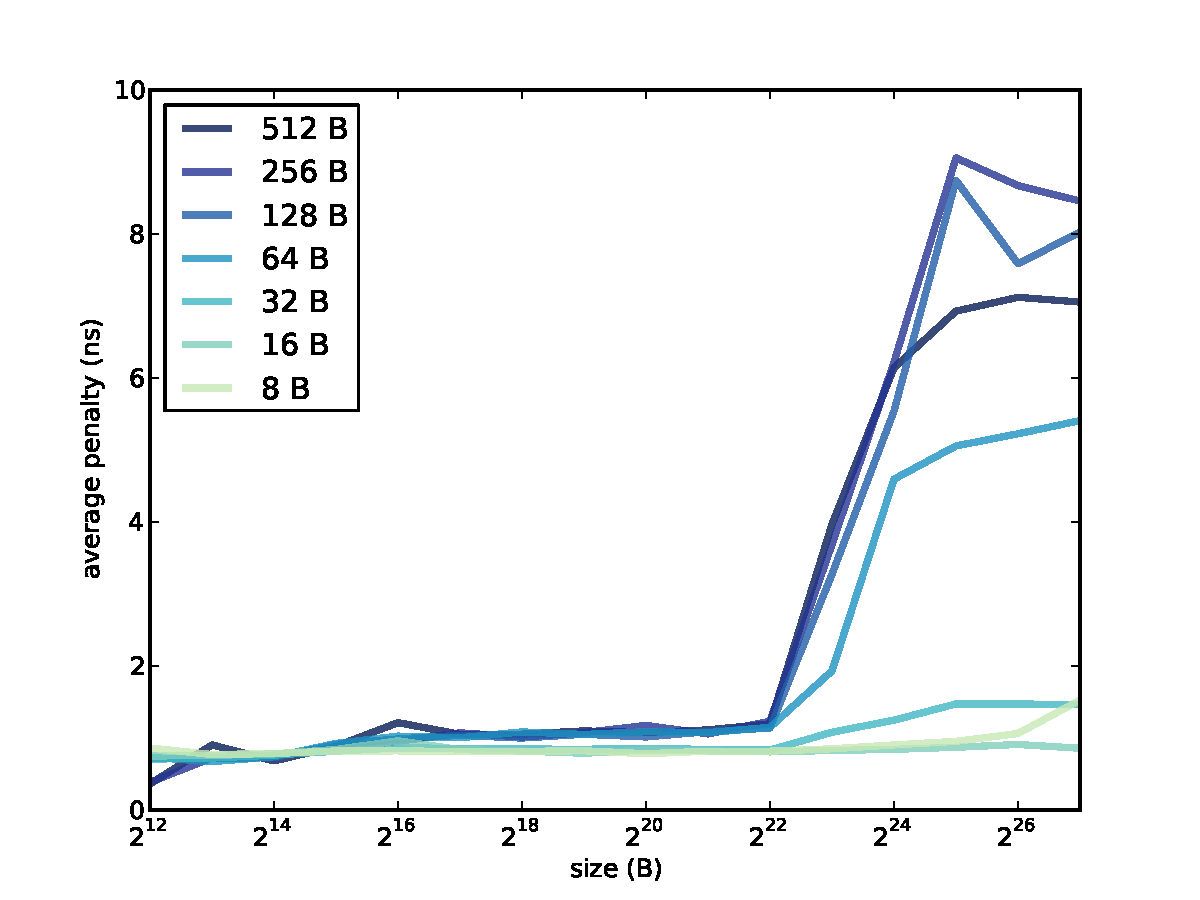
\includegraphics[width=3in]{figs/cache_data.pdf}}
%\caption{Average miss penalty as a function of array size and stride.}
\caption{数组大小和步长的平均缺失损失函数.}
\label{cachedata}
\end{figure}

%To isolate the time to access the elements of the array,
%the program runs a second loop that is almost identical except
%that the inner loop doesn't touch the array; it always increments
%the same variable:
为了排除访问数组元素的时间, 程序运行了第二个循环, 和第一个循环几乎相同, 唯一的差异在于内部循环不涉及数组; 其始终递增同一个变量:

\begin{verbatim}
    iters2 = 0;
    do {
        sec0 = get_seconds();
        
        for (index = 0; index < limit; index += stride) 
            temp = temp + index;
        
        iters2 = iters2 + 1;
        sec = sec - (get_seconds() - sec0);

    } while (iters2 < iters);
\end{verbatim}

%The second loop runs the same number of iterations as the first.
%After each iteration, it {\em subtracts} the elapsed time from
%{\tt sec}.  When the loop completes, {\tt sec} contains the total
%time for all array accesses, minus the total time it took to increment
%{\tt temp}.  This difference is the total miss penalty incurred by
%all accesses.  Finally, we divide by the number of accesses to
%get the average miss penalty per access, in ns:
第二个循环与第一个循环迭代相同次数. 
每次迭代之后, 它从 {\tt sec}变量中 {\em 减去} 经过的时间. 
当循环结束, {\tt sec} 包含所有数组访问的总时间, 减去递增 {\tt temp} 
花费的时间. 这个差值便是所有访问产生的总缺失损失. 
最后, 我们通过除以访问次数, 得到每次访问的平均缺失损失, 单位为纳秒:


\begin{verbatim}
sec * 1e9 / iters / limit * stride
\end{verbatim}

%If you compile and run {\tt cache.c} you should see output like this:
如果你编译并运行{\tt cache.c}, 你会看到如下输出:

\begin{verbatim}
Size:    4096 Stride:       8 read+write: 0.8633 ns
Size:    4096 Stride:      16 read+write: 0.7023 ns
Size:    4096 Stride:      32 read+write: 0.7105 ns
Size:    4096 Stride:      64 read+write: 0.7058 ns
\end{verbatim}

%If you have Python and {\tt matplotlib} installed, you can use
%\verb"graph_data.py" to graph the results.  Figure~\ref{cachedata}
%shows the results when I ran it on a Dell Optiplex 7010.
%Notice that the array size and stride are reported in
%bytes, not number of array elements.
如果您已安装Python和{\tt matplotlib} , 便可以使用\verb"graph_data.py"
来绘制结果. 图~\ref{cachedata}展示了我在戴尔Optiplex 7010上运行时的结果.
请注意, 数组大小和步长的单位是字节, 而不是数组元素的数量。

%Take a minute to consider this graph, and see what you can infer
%about the cache.  Here are some things to think about:
花一分钟来考虑这个图表, 看看您能从中推断出哪些关于缓存的信息. 
以下是一些需要考虑的事项:

\begin{itemize}

%\item The program reads through the array many times, so it has plenty
%  of temporal locality.  If the entire array fits in cache, we expect
%  the average miss penalty to be near 0.
\item 程序会遍历多次数组, 所以会有大量的时间局部性. 如果缓存包含了
全部数据, 我们便可以预计平均缺失损失接近于0.

%\item When the stride is 4 bytes, we read every element of the array,
%  so the program has plenty of spatial locality.  If the block size is
%  big enough to contain 64 elements, for example, the hit rate would
%  be 63/64, even if the array does not fit in cache.
  \item 当步长为4个字节, 我们会读取数组每个元素, 所以程序具有大量
  空间局部性. 如果块大小足够容纳64个元素, 即使缓存没有容纳整个数组, 
  命中率也是63/64.

%\item If the stride is equal to the block size (or greater), the
%  spatial locality is effectively zero, because each time we read a
%  block, we only access one element.  In that case we expect to see
%  the maximum miss penalty.
 \item 如果步长等于(或大于)块大小, 则空间局部性为零, 因为我们每次
 读取一个块, 仅仅需要访问一个元素. 如此情况, 我们可以预期会
 看到最大的缺失损失.

\end{itemize}

%In summary, we expect good cache performance if the array is smaller
%than the cache size {\em or} if the stride is smaller than the block
%size.  Performance only degrades if the array is bigger than the
%cache {\em and} the stride is large.
总之, 如果数组小于内存大小{\em 或}步长小于块大小, 我们便可以相信
内存性能良好. 只有当数组大于内存大小{\em 且}步长较大时, 性能才会
下降. 

%In Figure~\ref{cachedata}, cache performance is good, for all strides,
%as long as the array is less than $2^{22}$ B.  We can infer that the
%cache size is near 4 MiB; in fact, according to the specs, it is 3
%MiB.
图~\ref{cachedata}中, 只要数组小于$2^{22}$ B, 对于所有步长, 内存
性能都很好. 我们可以推断缓存大小接近 4 MiB; 实际上, 根据规格, 
是 3 MiB.

%When the stride is 8, 16, or 32 B, cache performance is good.  At 64 B
%it starts to degrade, and for larger strides the average miss
%penalty is about 9 ns.  We can infer that the block size near 128 B.
当步长是8, 16, 或 32 B时, 缓存性能良好. 当步长64B时, 性能开始下降, 
对于较大的步长, 内存损失大约9纳秒. 我们可以推断块大小接近128B. 

%Many processors use ``multi-level caches'' that include a small,
%fast cache and a bigger, slower cache.  In this example, it looks 
%like the miss penalty increases a little when the array size is bigger
%than $2^{14}$ B, so it's possible that this processor also has a 16 KB
%cache with an access time less than 1 ns.
很多处理器使用 ``多级缓存'',  其中包括一个小而快的缓存和一个大而慢
的缓存. 在这个示例中, 当数组大小大于$2^{14}$ B时, 缺失损失会略有
增加, 所以很可能处理器还有一个16KB的缓存, 其访问时间小于1纳秒.


%\section{Programming for cache performance}
\section{缓存性能编程}

%Memory caching is implemented in hardware, so most of the time
%programmers don't need to know much about it.  But if you know how
%caches work, you can write programs that use them more effectively.
内存缓存是通过硬件实现, 所以多数时候, 程序员不需要对其了解太多.
但如果知道缓存的工作原理, 你可以写出更高效使用缓存的程序代码. 

%For example, if you are working with a large array, it might be
%faster to traverse the array once, performing several operations with
%each element, rather than traversing the array several times.
例如, 假设你正在处理一个大数组, 对其进行一次遍历, 
同时对每个元素执行数个操作, 相比对数组遍历多次要更快一些.

%If you are working with a 2-D array, it might be stored as an array
%of rows.  If you traverse through the elements, it would be faster
%to go row-wise, with stride equal to the element size, rather
%than column-wise, with stride equal to the row length.
如果你正在处理一个行存储的二维数组, 那么你遍历数组时, 
逐行操作, 同时步长等于元素大小, 相比于逐列操作, 步长等于行
长度的遍历方式, 要更快一些.

%Linked data structures don't always exhibit spatial locality, because
%the nodes aren't necessarily contiguous in memory.  But if you allocate
%many nodes at the same time, they are usually co-located in the heap.
%Or, even better, if you allocate an array of nodes all at once, you
%know they will be contiguous.
链式数据结构并不总是表现出空间局部性, 因为节点在内存中并不一定
是连续的. 但如果你一次性分配了很多节点,它们通常在堆的相邻位置.
或者, 更好的操作是, 你分配一个节点数组, 你便知道他们会是连续的. 

%Recursive strategies like mergesort often have good cache behavior
%because they break big arrays into smaller pieces and then work
%with the pieces.  Sometimes these algorithms can be tuned to take
%advantage of cache behavior.
递归策略, 例如归并排序, 通常都有很好的缓存操作, 因为他们会将大数组
拆成小片段处理. 有时候这些算法还可以通过微调来更充分地利用缓存操作.

%For applications where performance is critical, it is possible
%to design algorithms tailored to the size of the cache, the block size,
%and other hardware characterstics.  Algorithms like that are
%called ``cache-aware''.  The obvious drawback of cache-aware
%algorithms is that they are hardware-specific.
对于性能优先的应用来说, 可以针对缓存大小, 块大小, 以及其他硬件
特性来设计算法. 这样的算法叫做``缓存感知''算法. 
而缓存感知算法的明显缺点则是他们是针对特定硬件的.

%\section{The memory hierarchy}
\section{内存层次架构}

%At some point during this chapter, a question like the following
%might have occurred to you: ``If caches are so much faster than
%main memory, why not make a really big cache and forget about
%memory?''
在本章的某个节点, 你可能会遇到如下问题: ``如果缓存比内存要
快很多, 为什么不制造一个足够大的缓存来替代内存?''

%Without going too far into computer architecture, there are two
%reasons: electronics and economics.  Caches are fast because they are
%small and close to the CPU, which minimizes delays due to capacitance
%and signal propagation.  If you make a cache big, it will be slower.
在不涉及过多计算机架构的情况下, 有两个原因: 电子学和经济学. 
缓存很快是因为它们小同时靠近CPU, 这便最小化了因电容和信号传播而造成
的延迟. 如果你制造一个大缓存, 速度便会慢很多.

%Also, caches take up space on the processor chip, and bigger chips are
%more expensive.  Main memory is usually dynamic random-access memory
%(DRAM), which uses only one transistor and one capacitor per bit, so
%it is possible to pack more memory into the same amount of space.  But
%this way of implementing memory is slower than the way caches are
%implemented.
此外, 缓存占据了处理器芯片上的空间, 而更大的芯片往往更加昂贵.
主存通常是动态随机访问存储(DRAM), 每比特只需要一个晶体管和一个电容, 
所以可以在相同空间内装入更多的内存. 但这种内存实现方式比缓存的
实现方式在速度上要慢很多.

% translator's note
\begin{note}
位和比特的翻译实在令我头疼, 后续将再次更正和优化.
\end{note}

%Also main memory is usually packaged in a dual in-line memory module
%(DIMM) that includes 16 or more chips.  Several small chips are cheaper
%than one big one.
此外, 主内存通常封装在一个双列直插内存模块(DIMM)中, 这个模块包括16个
或者更多的芯片. 而多个小芯片相比一个大芯片价格上要更加便宜.

%The trade-off between speed, size, and cost is the fundamental reason
%for caching.  If there were one memory technology that was fast,
%big, and cheap, we wouldn't need anything else.
速度, 大小和成本之间的权衡是缓存实现的根本原因. 
如果有一种快速, 容量大而且便宜的内存技术, 那我们便无需其他考虑了. 

%The same principle applies to storage as well as memory.  Solid state drives (SSD) are fast, but they are more expensive than hard drives (HDD), so they tend to be smaller.  Tape drives are even slower than hard
%drives, but they can store large amounts of data relatively
%cheaply.
这个原则同样适用于存储和内存. 固态硬盘(SSD)速度很快, 但相比于
硬盘驱动器(HDD)更加昂贵, 所以倾向于更小. 磁带驱动器比硬盘驱动器
更慢, 但它们可以相对廉价地存储大量数据.

%The following table shows typical access times, sizes, and 
%costs for each of these technologies.  
下表展示了每种技术的访问时间, 容量以及成本.

\vspace{0.1in}
\begin{center}
    \begin{tabular}{| l | l | l | l |}
    \hline
    设备   &   访问   &   典型    &   成本   \\
             &   时间     &   容量       &          \\ \hline
    寄存器(Register) &   0.5 ns   &   256 B      &   ?      \\ \hline
    缓存(Cache)    &   1 ns     &   2 MiB      &   ?      \\ \hline
    动态随机访问存储(DRAM)     &   100 ns   &   4 GiB      &   \$10 / GiB       \\ \hline
    固态硬盘(SSD)      &   10 \mus  &   100 GiB    &   \$1 / GiB      \\ \hline
    硬盘驱动器(HDD)      &   5 ms     &   500 GiB    &   \$0.25 / GiB     \\ \hline
    磁带(Tape)     &   minutes  &   1--2 TiB   &   \$0.02 / GiB      \\ \hline
    \end{tabular}
\end{center}
\vspace{0.1in}

\begin{note}
对于一些常用词汇,例如{\tt minutes}, {\tt ns} 等, 如果也强求翻译,
那我建议先补充一下英文基础知识.
\end{note}


%The number and size of registers depends on details of the
%architecture.  Current computers have about 32 general-purpose
%registers, each storing one ``word''.  On a 32-bit computer, a word
%is 32 bits or 4 B.  On a 64-bit computer, a word is 64 bits or 8 B.
%So the total size of the register file is 100--300 B.
寄存器的数量和大小取决于架构的细节. 当前的计算机拥有大约32个
通用寄存器, 每个存储一个``单词''. 在32位计算机上, 一个单词是32比特
或4字节. 在64位计算机上, 一个单词是64比特或8字节. 
所以寄存器文件的总大小是100--300字节.

%The cost of registers and caches is hard to quantify.  They contribute
%to the cost of the chips they are on, but consumers don't see that
%cost directly.
寄存器和缓存的成本是很难量化的. 它们会增加芯片的成本, 而消费者
很难直接看到这些费用. 

%For the other numbers in the table, I looked at the specifications for
%typical hardware for sale from online computer hardware stores.  By
%the time you read this, these numbers will be obsolete, but they give
%you an idea of what the performance and cost gaps looked like at one
%point in time.
对于表中的其他数字, 我查阅了在线计算机硬件商店中销售的典型硬件
的规格信息. 当你阅读本书时, 这些数字可能已经过时, 但它们可以让你
了解, 在某个时间节点, 不同硬件的性能和成本之间的差距是什么样子.

%These technologies make up the ``memory hierarchy'' (note that this
%use of ``memory'' also includes storage).  Each
%level of the hierarchy is bigger and slower than the one above it.
%And in some sense, each level acts as a cache for the one below
%it.  You can think of main memory as a cache for programs and data
%that are stored permanently on SSDs and HHDs.  And if you are working
%with very large datasets stored on tape, you could use hard drives
%to cache one subset of the data at a time.
这些技术构成了``内存层次结构''(注意, 此处的``内存''也包括存储).
层次结构中的每一层级相比于上一层级都要更大, 更慢. 某种意义上, 
每层都充当了下一层的缓存. 你可以将主存看作固态硬盘和硬盘驱动器
上永久存储的程序和数据的缓存. 
如果你正在处理存储在磁带上的大型数据集, 
你可以使用硬盘驱动器来逐次缓存单个数据子集.

%\section{Caching policy}
\section{缓存策略}

%The memory hierarchy suggests a framework for thinking about
%caching.  At every level of the hierarchy, we have to address
%four fundamental questions of caching:
内存层次结构提出了一个缓存思维框架. 在每个层级, 我们都需要解决
四个基本的缓存问题: 

\begin{itemize}

%\item Who moves data up and down the hierarchy?  At the top of the
%  hierarchy, register allocation is usually done by the compiler.
%  Hardware on the CPU handles the memory cache.  Users implicitly move
%  data from storage to memory when they execute programs and open
%  files.  But the operating system also moves data back and forth
%  between memory and storage.  At the bottom of the hierarchy,
%  administrators move data explicitly between disk and tape.
\item 谁负责在层次结构中上下移动数据? 在层次结构顶部, 寄存器的分配
通常由编译器完成. CPU 上的硬件会处理内存缓存. 当用户执行程序和
打开文件时, 数据会默默地从存储移动到内存中. 但操作系统也会在
内存和存储之间来回移动数据. 在层次结构的底部, 管理员需要清楚地
在磁盘和磁带之间移动数据.

%\item What gets moved?  In general, block sizes are small at the top
%  of the hierarchy and bigger at the bottom.  In a memory cache, a
%  typical block size is 128 B.  Pages in memory might be 4 KiB, but
%  when the operating system reads a file from disk, it might read 10s
%  or 100s of blocks at a time.
\item 移动了什么? 通常层次结构顶层的块较小, 底层块较大.
在缓存中, 一个典型的块大小是128 B. 内存中的页大小是 4KiB, 
但操作系统从磁盘读取一个文件时,  它可能一次读取10个或100个块.

%\item When does data get moved?  In the most basic cache, data gets
%  moved into cache when it is used for the first time.  But many
%  caches use some kind of ``prefetching'', meaning that data is
%  loaded before it is explicitly requested.  We have already seen
%  one form of prefetching: loading an entire block when only part of
%  it is requested.
\item 什么时候移动数据? 在最基本的缓存中, 数据首次使用时会被
移动进缓存. 但很多缓存会使用某种形式的``预取'', 意味着数据在被
明确请求之前便被加载. 我们已经看到过一种预取方式: 当只请求部分
块时也会加载整个块. 

%\item Where in the cache does the data go?  When the cache is full, we
%  can't bring anything in without kicking something out.  Ideally,
%  we want to keep data that will be used again soon and replace data
%  that won't.
\item 数据在缓存的哪个地方? 当缓存满了, 我们便需要先清除一些数据, 
才能再次添加数据({\tt 欲先添之, 必先减之}). 
理想情况是, 我们希望保留即将再次使用的数据, 替掉我们不再使用的数据.

\end{itemize}

%The answers to these questions make up the ``cache policy''.
%Near the top of the hierarchy, cache policies tend to be simple
%because they have to be fast and they are implemented in hardware.
%Near the bottom of the hierarchy, there is more time to make decisions,
%and well-designed policies can make a big difference.
这些问题的答案构成了``缓存机制''. 在层次结构顶部附近, 
缓存机制往往简单, 因为它们必须要快速, 并能用硬件实现. 
靠近层次结构底部, 可以有更多的决策时间, 而设计良好的策略
则会影响重大.

%Most cache policies are based on the principle that history repeats
%itself; if we have information about the recent past, we can use it to
%predict the immediate future.  For example, if a block of data has
%been used recently, we expect it to be used again soon.  This
%principle suggests a replacement policy called ``least recently
%used,'' or LRU, which removes from the cache a block of data that
%has not been used recently.  For more on this topic, see
%\url{http://en.wikipedia.org/wiki/Cache_algorithms}.
大部分的缓存机制基于历史重演的原则; 如果我们有近期的历史信息,
我们便可以用它预测不久的将来. 例如, 如果一个数据块最近被使用了, 
我们可以预期它很快会再次被使用. 这个原则引出了一个替换策略, 叫做
``最近最少使用''策略, 或 LRU, 这个策略会将缓存中最近未被使用的
数据块移除. 有关此主题的更多信息, 请参阅\url{http://en.wikipedia.org/wiki/Cache_algorithms}.


%\section{Paging}
\section{分页}
\label{paging}

%In systems with virtual memory, the operating system can move
%pages back and forth between memory and storage.  As I mentioned
%in Section~\ref{leak}, this mechanism is called ``paging'' or
%sometimes ``swapping''.
在具有虚拟内存的系统中, 操作系统可以在内存和存储之间来回移动页面.
如我在Section~\ref{leak}节提到的, 这个机制称作``分页'', 有时也叫做
``交换''.

%Here's how the process works:
下面是这个过程的工作原理:

\begin{enumerate}

%\item Suppose Process A calls {\tt malloc} to allocate a chunk.  If there
%is no free space in the heap with the requested size, {\tt malloc} calls
%{\tt sbrk} to ask the operating system for more memory.
\item 假设进程A调用{\tt malloc}分配一块内存. 如果堆中没有足够大小
的空闲空间, {\tt malloc} 会调用{\tt sbrk}来请求操作系统分配更多内存.

%\item If there is a free page in physical memory, the operating system
%adds it to the page table for Process A, creating a new range of valid
%virtual addresses.
\item 如果物理内存中有一个空闲页, 操作系统会将其添加到进程A的页表
中, 创建一个新的有效虚拟地址范围.

%\item If there are no free pages, the paging system chooses a ``victim
%page'' belonging to Process B.  It copies the contents of the victim
%page from memory to disk, then it modifies the page table for Process
%B to indicate that this page is ``swapped out''.
\item 如果没有空闲页, 分页系统会选择一个属于进程B的``受害页''. 将受害页中的内容从内存复制到磁盘, 然后修改进程B的页表, 表明该页
已被``交换出去''.

%\item Once the data from Process B is written, the page can be reallocated
%to Process A.  To prevent Process A from reading Process B's data, the
%page should be cleared.
\item 一旦进程B的数据被写入, 该页便可以被重新分配给进程A. 为了防止
进程A读取进程B的数据, 该页应该被清空.

%\item At this point the call to {\tt sbrk} can return, giving {\tt malloc}
%additional space in the heap.  Then {\tt malloc} allocates the requested
%chunk and returns.  Process A can resume.
\item 此时, 对 {\tt sbrk} 的调用便可以返回, 在堆中为{\tt malloc}提供额外
空间. 然后{\tt malloc} 分配请求的内存块并返回, 进程A可以继续. 

%\item When Process A completes, or is interrupted, the scheduler might
%allow Process B to resume.  When Process B accesses a page that has been swapped out, the memory management unit notices that the page is ``invalid'' and causes an interrupt.
\item 当进程A完成, 或被中断, 调度器可能会允许进程B继续. 当进程B访问
一个已被交换出去的页时, 内存管理单元会注意到该页是``无效''的, 并引发
一个中断.

%\item When the operating system handles the interrupt, it sees that
%the page is swapped out, so it transfers the page back from disk to
%memory.  
\item 当操作系统处理中断时, 会发现该页已经被交换出去, 所以它会将
该页从磁盘转移到内存.

%\item Once the page is swapped in, Process B can resume.
\item 一旦该页被交换进来, 进程B便可以继续.

\end{enumerate}

%When paging works well, it can greatly improve the utilization of
%physical memory, allowing more processes to run in less space.
%Here's why:
当分页正常工作, 它可以极大提高物理内存的利用率, 允许更多进程在较少
空间运行. 原因如下:

\begin{itemize}

%\item Most processes don't use all of their allocated memory.  Many
%  parts of the text segment are never executed, or execute once and
%  never again.  Those pages can be swapped out without causing any
%  problems.
\item 大部分的进程不会使用分配给它们的全部内存. 文本段的许多部分
从不会被执行, 或者执行一次后再也不被执行. 这些页可以被交换出去
而不会引发任何问题.

%\item If a program leaks memory, it might leave allocated space behind
%  and never access it again.  By swapping those pages out, the
%  operating system can effectively plug the leak.
\item 如果程序存在内存泄漏, 可能会遗留被分配的空间, 再也不访问它.
通过交换这些页出去, 操作系统可以有效堵住内存泄漏.

%\item On most systems, there are processes like daemons that sit idle
%  most of the time and only occasionally ``wake up'' to respond to
%  events.  While they are idle, these processes can be swapped out.
\item 在大部分系统中, 有一些像守护进程那样, 大部分时间处于空闲状态,
只偶尔被``唤醒''以响应事件. 当这些处于空闲时, 可以被交换出去.

%\item A user might have many windows open, but only a few are active
%  at a time.  The inactive processes can be swapped out.
\item 用户可能打开了很多窗口, 但同一时间只有少数几个处于活动
状态. 那么不活跃的进程便可以被交换出去.

%\item Also, there might be many processes running the same program.
%  These processes can share the same text and static segments, avoiding the need to keep multiple copies in physical memory.
\item 此外, 可能有很多进程运行着相同程序. 这些进程可以共享同一文本
和静态段, 避免在物理内存中保留多个副本.

\end{itemize}

%If you add up the total memory allocated to all processes, it can
%greatly exceed the size of physical memory, and yet the system can
%still behave well.
如果你将分配给所有进程的内存相加, 可能远远超出物理内存的大小, 
但系统依然表现良好.

%Up to a point.
在一定程度上是这样的.

%When a process accesses a page that's swapped out, it has to get the
%data back from disk, which can take several milliseconds.  The
%delay is often noticeable.  If you leave a window idle for a long
%time and then switch back to it, it might start slowly,
%and you might hear the disk drive working while pages are
%swapped in.  
当进程访问交换出去的页时, 需要从磁盘获取数据, 而这会耗费几毫秒
的时间. 这种延迟通常是显而易见的. 如果你让一个窗口长时间处于
空闲, 然后突然切换回去, 也许会启动较慢, 你可能会在页交换回来时
听到磁盘驱动器运转起来.

%Occasional delays like that might be acceptable, but if you have too
%many processes using too much space, they start to interfere with each
%other.  When Process A runs, it evicts the pages Process B needs.
%Then when B runs, it evicts the pages A needs.  When this happens,
%both processes slow to a crawl and the system can become unresponsive.
%This scenario is called ``thrashing''.
偶尔出现这种延迟是可以接受的, 但如果你有太多的进程占用了太多的
空间, 它们会开始相互影响. 当进程A运行, 它会驱逐进程B需要的页. 
当进程B运行, 它又会驱逐进程A需要的页. 当这种情况发生, 两个进程
都会变得缓慢, 系统变得不响应. 这种现象叫做``抖动''.

%In theory, operating systems could avoid thrashing by detecting an
%increase in paging and blocking or killing processes until the system
%is responsive again.  But as far as I can tell, most systems don't do
%this, or don't do it well; it is often left to users to limit their
%use of physical memory or try to recover when thrashing occurs.
理论上, 操作系统可以通过检测页的增加, 并堵塞或者杀掉进程, 直到
系统再次响应, 来避免抖动. 但据我所知, 多数系统没有这样做, 或者做得
不好; 通常情况是让用户限制他们物理内存的使用, 或在抖动发生时, 尝试恢复而已.

\begin{note}
此处可以思考, 为什么多数操作系统不采取更有好的方式来避免抖动, 而是采取相对强硬或者暴力的措施?
\end{note}


%\chapter{Multitasking}
\chapter{多任务}

%In many current systems, the CPU contains multiple cores, which means
%it can run several processes at the same time.  In addition, each core
%is capable of ``multitasking'', which means it can switch from one
%process to another quickly, creating the illusion that many processes
%are running at the same time.
当前很多系统中, CPU包括多个核, 也就表示系统可以同时运行多个进程. 
另外, 每个核都能够进行``多任务处理'', 意味着可以从一个进程快速切换
到另一个进程, 从而产生多个进程同时运行的错觉. 

%The part of the operating system that implements multitasking is
%the ``kernel''.  In a nut or seed, the kernel is the innermost
%part, surrounded by a shell.  In an operating system, the kernel
%is the lowest level of software, surrounded by several other
%layers, including an interface called a ``shell.''  Computer
%scientists love extended metaphors.
操作系统实现多任务处理的部分是``内核''. 在坚果或种子中, 内核是最
内层的部分, 被壳所包围. 操作系统中, 内核是软件最底层的部分, 外部被
其他层环绕, 其中包括一个叫做``shell'' 的接口层. 
计算机专家往往喜欢使用这种类比的方式. 

%At its most basic, the kernel's job is to
%handle interrupts.  An ``interrupt'' is an event that stops the
%normal instruction cycle and causes the flow of execution to jump to a
%special section of code called an ``interrupt handler''.
在最基本的功能中, 内核的工作是处理中断. 一个``中断'' 就是一个事件, 
这个事件会停止正常指令周期, 并使执行流跳转到被称为``中断处理程序''
的特定代码部分.

%TODO: put new vocab in bold and add glossaries

%A {\bf hardware interrupt} is caused when a device sends a signal to the
%CPU.  For example, a network interface might cause an interrupt when
%a packet of data arrives, or a disk drive might cause an interrupt
%when a data transfer is complete.  Most systems also have timers that
%cause interrupts at regular intervals, or after an elapsed time.
 {\bf 硬件中断}是由设备向CPU发送信号引发的. 例如, 网络接口会在
 数据包到达时引起中断, 或着, 数据传输结束会, 磁盘驱动器也会触发中断.
 大部分的系统还有计时器会在定期, 或某段时间后触发中断.
 

%A {\bf software interrupt} is caused by a running program.  For example, if
%an instruction cannot complete for some reason, it might trigger an
%interrupt so the condition can be handled by the operating system.
%Some floating-point errors, like division by zero, are handled
%using interrupts.
{\bf 软件中断}通常由运行中的程序触发. 例如, 如果某个指令因为某种原因
无法完成, 便可能触发中断, 以便操作系统可以处理该状况. 有些浮点错误, 
比如除零操作, 也是通过中断来处理. 

%When a program needs to access a hardware device,
%it makes a {\bf system call}, which is similar to a function call,
%except that instead of jumping to the beginning of the function,
%it executes a special instruction that triggers an interrupt, causing
%the flow of execution to jump to the kernel.  The kernel reads the
%parameters of the system call, performs the requested operation,
%and then resumes the interrupted process.
当程序需要访问硬件设备时, 会进行一次{\bf 系统调用}, 类似于函数调用, 
但不同之处在于, 它不会跳转到函数的开头, 而是执行某个特殊指令触发
中断, 从而令执行流跳转到内核. 内核读取系统调用的参数, 执行请求的操作, 
然后恢复被中断的进程.


%\section{Hardware state}
\section{硬件状态}

%Handling interrupts requires cooperation between hardware and
%software.  When an interrupt occurs, there might be several
%instructions running on the CPU, data stored in registers, and
%other {\bf hardware state}.
处理中断需要硬件和软件之间的协作. 当中断发生时, 可能CPU正有多条
指令在运行, 寄存器中正存储着数据, 以及其他的{\bf 硬件状态}.

%Usually the hardware is responsible for bringing the CPU
%to a consistent state; for example, every instruction should either
%complete or behave as if it never started.  No instruction should
%be left half complete.  Also, the hardware is responsible for
%saving the program counter (PC), so the kernel knows where to
%resume.
通常, 硬件负责将CPU带到一个一致性的状态; 例如, 每个指令都应该完成, 
或者如同从未开始. 任何指令都不应该被留在半完成的状态. 此外, 硬件负责
保存程序计数器(PC), 以便内核知道从何处恢复. 

%Then, usually, it is the responsibility of the interrupt handler
%to save the rest of the hardware state before it does anything that
%might modify it, and then restore the saved state before the interrupted
%process resumes.
然后, 通常情况下, 中断处理程序需要在任何可能改变某个硬件状态的操作前, 
保存其余的硬件状态, 然后在被中断进程恢复前, 还原被保存的状态. 

%Here is an outline of this sequence of events:
以下是此事件序列的概要: 

\begin{enumerate}

%\item When the interrupt occurs, the hardware saves the program
%counter in a special register and jumps to the appropriate interrupt
%handler.
\item 当中断发生, 硬件将程序计数器保存在某个特殊的寄存器中, 
同时跳转到适当的中断处理程序. 

%\item The interrupt handler stores the program counter and the
%status register in memory, along with the contents of any data
%registers it plans to use.
\item 中断处理程序将程序计数器和状态寄存器, 以及计划使用的
数据寄存器的任何数据, 一并存储在内存中.

%\item The interrupt handler runs whatever code is needed to handle
%the interrupt.
\item 中断处理程序运行处理中断所需的所有代码. 

%\item Then it restores the contents of the saved registers.  Finally,
%it restores the program counter of the interrupted process, which
%has the effect of jumping back to the interrupted instruction.
\item 然后它会恢复保存的寄存器的内容. 最后, 它恢复中断程序的程序计数器, 
这会令执行流回到中断指令处. 

\end{enumerate}

%If this mechanism works correctly, there is generally no way for
%the interrupted process to know there was an interrupt, unless
%it detects the change in time between instructions.
如果这个机制运转正常, 通常情况下, 被中断的进程不会觉察到中断发生, 
除非它检测到指令间的事件变化.


%\section{Context switching}
\section{上下文切换}

%Interrupt handlers can be fast because they don't have to save the
%entire hardware state; they only have to save registers they are
%planning to use.
中断处理程序之所以快速, 是因为它们不必存储整个硬件状态; 只需要
存储它们后续使用的寄存器.

%But when an interrupt occurs, the kernel does not always resume the
%interrupted process.  It has the option of switching to another
%process.  This mechanism is called a ``context switch''.
但是当中断发生时, 内核并不总是会恢复中断的进程. 
它也可以切换到另一个进程. 这种机制叫做``上下文切换''.

%In general, the kernel doesn't know which registers a process will
%use, so it has to save all of them.  Also, when it switches to a new
%process, it might have to clear data stored in the memory management
%unit (see
%Section~\ref{address_translation}).  And after the context switch, it
%might take some time for the new process to load data into the cache.
%For these reasons, context switches are relatively slow, on the order
%of thousands of cycles, or a few microseconds.
一般来说, 内核并不知道进程要使用哪个寄存器, 所以需要保存所有寄存器. 
此外, 当内核切换到一个新的进程, 可能需要清理存储在内存管理
单元中的数据(见第~\ref{address_translation}节). 
在上下文切换后, 新进程需要一些时间将数据加载到缓存中. 
因此, 上下文切换相对较慢, 大约需要上千个时间周期, 或者几微秒. 

%In a multi-tasking system, each process is allowed to run for a short
%period of time called a ``time slice'' or ``quantum''.  During
%a context switch, the kernel sets a hardware timer that causes
%an interrupt at the end of the time slice.  When the interrupt
%occurs, the kernel can switch to another process or allow the
%interrupted process to resume.  The part of the operating system
%that makes this decision is the ``scheduler''.
在一个多任务系统中, 每个进程都会运行一小段时间, 这段时间称为
``时间片'' 或 ``量子''. 在上下文切换期间, 内核会设置一个硬件
定时器, 在时间片结束时引发中断. 当中断发生时, 内核可以切换到
另一个进程或者恢复中断的进程. 操作系统中做这一决策的部分叫做
``调度程序''.


%\section{The process life cycle}
\section{进程生命周期}

%When a process is created, the operating system allocates a
%data structure that contains information about the process, called
%a ``process control block'' or PCB.  Among other things, the
%PCB keeps track of the process state, which is one of:
当进程被创建时, 操作系统会分配一个包含进程相关信息的数据结构, 
被称作``进程控制块(process control block)'' 或 PCB. 
此外, PCB还会追踪进程状态, 其中如下:

\begin{itemize}

%\item Running, if the process is currently running on a core.
\item 运行状态, 即进程当前正在核心上运行.

%\item Ready, if the process could be running, but isn't, usually because
%there are more runnable processes than cores.
\item 就绪状态, 即进程可以运行但还未运行, 通常是因为
可运行的进程数超过了核心数.

%\item Blocked, if the process cannot run because it is waiting for
%a future event like network communication or a disk read.
\item 阻塞状态, 即进程暂时无法运行, 通常因要等待一个将来的事件, 
比如网络通信或磁盘读取.

%\item Done, if the process has completed, but has exit status
%information that has not been read yet.
\item 完成状态, 即进程已经完成, 但还有退出状态信息未被读取.

\end{itemize}

%Here are the events that cause a process to transition from one state to another:
下面是导致进程从一个状态转换到另一个状态的事件: 

\begin{itemize}

%\item A process is created when the running program executes a system
%  call like {\tt fork}.  At the end of the system call, the new
%  process is usually ready.  Then the scheduler might resume the
%  original process (the ``parent'') or start the new process (the
%  ``child'').
\item 当运行的程序执行类似 {\tt fork} 的系统调用时, 就会创建一个进程.
系统调用结束时, 新进程通常处于就绪状态. 然后调度程序会恢复
原始程序(``父进程'') 或者启动新进程(``子进程''). 

%\item When a process is started or resumed by the scheduler, its state
%  changes from ready to running.
\item 当一个进程被调度程序启动或恢复, 其状态便会从就绪变为运行.

%\item When a process is interrupted and the scheduler chooses not
%  to let it resume, its state changes from running to ready.

%\item If a process executes a system call that cannot complete
%  immediately, like a disk request, it becomes blocked
%  and the scheduler usually chooses another process.
\item 如果一个进程执行一个无法立刻完成的系统调用时, 像磁盘
请求, 便会被堵塞住, 同时调度程序通常会选择另一个进程执行. 

%\item When an operation like a disk request completes, it causes an
%  interrupt.  The interrupt handler figures out which process was
%  waiting for the request and switches its state from
%  blocked to ready.  Then the scheduler may or may not choose to
%  resume the unblocked process.
\item 当一个像磁盘请求这样的操作完成, 会触发中断. 中断处理程序
会确定等待该请求的进程, 并将其状态从堵塞切换为就绪. 然后
调度程序会选择是否恢复未堵塞的进程. 

%\item When a process calls {\tt exit}, the interrupt handler stores
%  the exit code in the PCB and changes the process's state to done.
\item 当一个进程调用 {\tt exit}, 中断处理程序会将退出码存储在PCB, 
并将进程状态更改为完成. 

\end{itemize}


%\section{Scheduling}
\section{调度}

%As we saw in Section~\ref{unixps} there might be hundreds of
%processes on a computer, but usually most of them are blocked.  Most
%of the time, there are only a few processes that are ready or running.
%When an interrupt occurs, the scheduler decides which process to start
%or resume.
正如在第~\ref{unixps}节中看到的, 计算机上可能有数百个进程, 但通常大多数进程都是被阻塞的。大多数时候, 只有少数进程处于就绪或运行状态. 当中断发生时, 调度程序决定启动或恢复某个进程。

%On a workstation or laptop, the primary goal of the scheduler is to
%minimize response time; that is, the computer should respond quickly
%to user actions.  Response time is also important on a server, but in
%addition the scheduler might try to maximize throughput, which is the
%number of requests that complete per unit of time.
在工作站或笔记本电脑上, 调度程序的主要目标是最小化响应时间, 也就是说,计算机应该对用户操作快速做出响应. 在服务器上, 响应时间也很重要, 但此外, 调度程序可能会尝试最大化吞吐量, 即单位时间内完成的请求数量.

%Usually the scheduler doesn't have much information about what
%processes are doing, so its decisions are based on a few
%heuristics:
通常,调度程序并不清楚进程正在做什么, 因此其决策基于一些启发式规则:


\begin{itemize}

%\item Processes might be limited by different resources.  A process
%that does a lot of computation is probably CPU-bound, which means that
%its run time depends on how much CPU time it gets.  A process that
%reads data from a network or disk might be I/O-bound, which means that
%it would run faster if data input and output went faster, but would not
%run faster with more CPU time.  Finally, a process that interacts with
%the user is probably blocked, most of the time, waiting for user actions.
\item 进程可能受限于不同的资源. 进行大量计算的进程是CPU密集型, 
表示其运行时间取决于取得的CPU时间. 从网络或磁盘读取数据的进程是
I/O密集型, 意味着如果数据输入输出速度越快, 便运行越快, 但即使取得
更多CPU时间, 也不会更快. 最后, 与用户交互的进程很可能会被堵塞, 
其大部分时间在等待用户操作.
%\item 進程可能會受到不同資源的限制。進行大量運算的進程可能是CPU密集型的,這意味著其執行時間取決於獲得的CPU時間。從網路或磁碟讀取資料的進程可能是I/O密集型的,這意味著如果資料輸入和輸出速度更快,它將執行得更快,但不會因為更多的CPU時間而執行得更快。最後,與使用者互動的進程可能大部分時間都在等待使用者操作而被阻塞。

%The operating system can sometimes classify processes based on their
%past behavior, and schedule them accordingly.  For example, when an
%interactive process is unblocked, it should probably run immediately,
%because a user is probably waiting for a reply.  On the other hand,
%a CPU-bound process that has been running for a long time might be
%less time-sensitive.
操作系统有时可以根据进程过去的行为, 对其进行分类, 并进行相应
调度. 例如, 当一个交互进程解除堵塞时, 它应该立刻运行, 因为用户
可能正在等待一个回复. 另一方面, 一个长时间运行的CPU密集型进程,
对于时间便不再敏感.
%作業系統有時可以根據程序過去的行為對其進行分類,並相應地進行排程。例如,當一個互動式程序被解除阻塞時,它可能應該立即執行,因為使用者可能正在等待回覆。另一方面,一個長時間執行的CPU密集型程序可能不太時間敏感。

%\item If a process is likely to run for a short time and then make
%a blocking request, it should probably run immediately, for two reasons:
%(1) if the request takes some time to complete, we should start it as soon
%as possible, and (2) it is better for a long-running process to wait
%for a short one, rather than the other way around.
\item 如果一个进程可能只会运行一小段时间, 然后会发出一个阻塞请求, 它可能应该立即运行, 原因有二: (1) 如果请求需要一些时间才能完成, 我们应该尽快开始; (2) 让一个耗时长的进程等待一个耗时短的进程, 要比反过来好很多. 

%As an analogy, suppose you are making an apple pie.  The crust takes
%5 minutes to prepare, but then it has to chill for half an hour.  It takes
%20 minutes to prepare the filling.  If you prepare the crust first,
%you can prepare the filling while the crust is chilling, and you can
%finish the pie in 35 minutes.  If you prepare the filling first, the
%process takes 55 minutes.
打个比方, 假设你正在做苹果派. 准备外皮需要5分钟, 但之后需要冷藏半小时. 准备馅料需要20分钟. 如果你先准备外皮, 你可以在外皮冷藏的时候准备馅料, 35分钟就可以完成苹果派. 如果你先准备馅料, 整个过程需要55分钟. 

\begin{note}
好比制作包子, 和面需要5分钟, 之后醒面需要半小时, 准备馅需要20分钟. 如果先和面, 而后在醒面的时候准备馅, 35分钟即可完成. 如果你先弄馅, 你需要55分钟才能完成.
\end{note}

\end{itemize}

%Most schedulers use some form of priority-based scheduling,
%where each process has a priority that can be adjusted up or down
%over time.  When the scheduler runs, it chooses the runnable process
%with the highest priority.
多数调度程序使用基于优先级的调度策略, 其中每个进程都有一个根据时间
变化调整的优先级. 当调度程序运行时, 它会选择具有最高优先级的可运行进程.  

%Here are some of the factors that determine a process's priority:
以下是确定进程优先级的一些因素: 

\begin{itemize}

%\item A process usually starts with a relatively high priority so it
%  starts running quickly.
\item 进程通常以相对较高的优先级启动, 以便快速开始运行.

%\item If a process makes a request and blocks before its time slice is
%  complete, it is more likely to be interactive or I/O-bound, so its
%  priority should go up.
\item 如果进程在它的时间片结束前, 产生了请求并堵塞, 很可能是因为交互
或I/O密集, 因此其优先级应该提高.

%\item If a process runs for an entire time slice, it is more likely to
%  be long-running and CPU-bound, so its priority should go down.
\item 如果一个进程运行了整个时间片, 它很可能是长时间运行且CPU
密集, 所以其优先级应该降低.


%\item If a task blocks for a long time and then becomes ready, it
%  should get a priority boost so it can respond to whatever it was
%  waiting for.
\item 如果一个任务堵塞较长时间后, 变为就绪状态, 它应该获得优先级
提升, 以便其能快速响应等待的任意事件. 
%
%\item If process A is blocked waiting for process B, for example if
%  they are connected by a pipe, the priority of process B should go
%  up.
\item 如果A进程因等待B进程而被堵塞, 例如, 它们通过管道连接, B进程的
优先级应该提高.


%\item The system call {\tt nice} allows a process to decrease (but not
%  increase) its own priority, allowing programmers to pass explicit
%  information to the scheduler.
\item 通过{\tt nice}系统调用, 进程可以降低(而不是提高)其自身优先级, 程序员也可以向调度程序显式传递信息, 从而对进行优先级进行调整. 

\end{itemize}

%For most systems running normal workloads, scheduling algorithms
%don't have a substantial effect on performance.  Simple scheduling
%policies are usually good enough.
对多数负载正常的系统来说, 调度算法对性能没有实质性的影响. 
通常简单的调度策略已绰绰有余. 

%\section{Real-time scheduling}
\section{实时调度}

%However, for programs that interact with the real world, scheduling
%can be very important.  For example, a program that reads data from
%sensors and controls motors might have to complete recurring tasks at
%some minimum frequency and react to external events with some maximum
%response time.  These requirements are often expressed in terms of
%``tasks'' that must be completed before ``deadlines''.
然而, 对于与现实世界交互的程序来说, 调度非常重要. 例如, 一个从传感器
读取数据并控制电机的程序, 可能需要以最小频率完成重复任务, 并在某个
最大响应时间限制内完成外部事件的响应. 这些要求通常用必须在``截止日期'' 内完成的``任务''来表示.

%Scheduling tasks to meet deadlines is called ``real-time
%  scheduling''.  For some applications, a general-purpose operating
%system like Linux can be modified to handle real-time scheduling.
%These modifications might include:
调度任务以满足截止时间, 称做``实时调度''. 对于某些应用来说, 像Linux这种
通用操作系统可以通过修改, 满足实时调度. 这些更改可能包括: 

\begin{itemize}

%\item Providing richer APIs for controlling task priorities.
\item 为任务优先级控制提供丰富API. 

%\item Modifying the scheduler to guarantee that the process with
%highest priority runs within a fixed amount of time.
\item 修改调度器, 确保最高优先级的进程拥有固定时间. 

%\item Reorganizing interrupt handlers to guarantee
%a maximum completion time.
\item 重新调整中断处理程序, 以保证最大完成时间. 

%\item Modifying locks and other synchronization mechanisms (coming up
%  in the next chapter) to allow a high-priority task to preempt a
%  lower-priority task.
\item 修改锁以及其他同步机制(下一章介绍), 以允许高优先级任务可以抢占
低优先级任务资源. 

%\item Choosing an implementation of dynamic memory allocation that
%guarantees a maximum completion time.
\item 选择能保证最大完成时间的动态内存分配实现. 

\end{itemize}

%For more demanding applications, especially in domains where real-time
%response is a matter of life and death, ``real-time operating
%  systems'' provide specialized capabilities, often with much simpler
%designs than general purpose operating systems.
对于更加苛刻的应用, 特别是实时响应关乎生死存亡的领域, 
``实时操作系统'' 提供了专门的能力, 通常比通用操作系统拥有
更加简洁的设计. 

\begin{note}
实现实时操作系统, 需要对中断处理, 以及不同优先级的进程进行
极为精细的时间控制, 避免超出最大完成时间, 从而保证操作系统的
实时性能.

例如在电力行业应用的操作系统, 对实时性要求很高, 因为一旦电路出现
问题, 即使系统响应延迟几毫秒, 在电的高速传输下, 也会影响到数百公里, 
甚至上千公里的范围.
\end{note}

%TODO: kernel mode?  signals?  user and system time


%\chapter{Threads}
\chapter{线程}

%When I mentioned threads in Section~\ref{unixps}, I said that a thread
%is a kind of process.  Now I will provide a more careful explanation.
当我在第~\ref{unixps}节提到线程时, 我说线程就是一种进程. 
现在我会提供一种更加谨慎的解释.

%When you create a process, the operating system creates a new address
%space, which includes the text segment, static segment, and heap; it
%also creates a new ``thread of execution'', which includes the program
%counter and other hardware state, and the call stack.
当你创建一个进程时, 操作系统会创建一个新的地址空间, 其中包括文本段, 
静态段, 以及堆; 也会创建一个新的``执行线程'', 其包括程序计数器和其他
硬件状态, 以及调用堆栈. 

%The processes we have seen so far are ``single-threaded'', which means
%that only one thread of execution runs in each address space.  In this
%chapter, you will learn about ``multi-threaded'' processes that have
%multiple threads running in the same address space.
我们目前见到的进程都是``单线程的'', 也就是说每个地址空间中仅运行一个
执行线程. 本章中, 我们会学习 ``多线程的'' 进程, 即同一地址空间中运行多个线程的进程.   

%Within a single process, all threads share the same text segment, so
%they run the same code.  But different threads often run different parts
%of the code.
在单个进程内, 所有线程共享相同的文本段, 因此它们执行相同的
代码. 但不同的线程通常执行代码的不同部分. 

%And they share the same static segment, so if one thread changes a
%global variable, other threads see the change.  They also share the heap,
%so threads can share dynamically-allocated chunks.
同时, 它们共享同样的静态段, 所以如果一个线程修改了一个全局变量, 
其他线程也会看到变化. 它们还共享堆, 所以线程可以共享动态分配的块. 


%But each thread has its own stack, so threads can call functions without
%interfering with each other.  Usually threads don't access each
%other's local variables (and sometimes they can't).
但每个线程拥有自己的堆栈, 因此线程可以互不干扰地调用函数. 
通常线程不会访问彼此的局部变量(有时候它们也不能).

%The example code for this chapter is in the repository for this book,
%in a directory named {\tt counter}.  For information on downloading
%this code, see Section~\ref{code}.
本章的样例代码在本书的代码仓库中, 名为 {\tt counter}的目录下. 
有关下载代码的更多信息, 见第~\ref{code}节.

%\section{Creating threads}
\section{创建线程}

%The most popular threading standard used with C is POSIX Threads, or Pthreads for short.  The POSIX standard defines a thread model and an interface for creating and controlling threads.  Most versions of UNIX provide an implementation of Pthreads.
在C语言中, 最流行的线程标准是POSIX线程, 简称为Pthread. 
POSIX标准定义了一个线程模型, 以及创建和控制线程的接口. 
多数UNIX版本都提供了Pthread的实现.

%Using Pthreads is like using most C libraries:
使用Pthread就像使用多数C库一样:

\begin{itemize}

%\item You include headers files at the beginning of your
%program.
\item 在程序的开头包括头文件.

%\item You write code that calls functions defined by Pthreads.
\item 编写调用基于Pthread定义的函数代码.

%\item When you compile the program, you link it with the Pthread library.
\item 当编译程序时, 将其与Pthread库链接. 

\end{itemize}

%For my examples, I include the following headers:
比如我的例子, 包含以下头文件: 

\begin{verbatim}
#include <stdio.h>
#include <stdlib.h>
#include <pthread.h>
#include <semaphore.h>
\end{verbatim}

%The first two are standard; the third is for Pthreads and
%the fourth is for semaphores.  To compile with the Pthread library in {\tt gcc}, you can use the {\tt -l} option on the command line:
前两个是标准库; 第三个是用于Pthreads的, 第四个是用于信号量的.
若要在{\tt gcc}中使用Pthread库编译, 你可以在命令行使用 {\tt -l} 选项:

\begin{verbatim}
gcc -g -O2 -o array array.c -lpthread
\end{verbatim}

%This compiles a source file named {\tt array.c} with debugging info
%and optimization, links with the Pthread library, and generates an
%executable named {\tt array}.
这将编译名为{\tt array.c} 的源文件, 包含调试信息和优化, 链接Pthread库, 
以及生成名为{\tt array}的可执行文件.


%\section{Creating threads}
\section{创建线程}

%The Pthread function that creates threads is called \verb"pthread_create".
%The following function shows how to use it:
创建线程的Pthread函数叫做\verb"pthread_create".
下面函数展示了如何使用它:

\begin{verbatim}
pthread_t make_thread(void *(*entry)(void *), Shared *shared)
{
    int n;
    pthread_t thread;

    n = pthread_create(&thread, NULL, entry, (void *)shared);
    if (n != 0) {
        perror("pthread_create failed");
        exit(-1);
    }
    return thread;
}
\end{verbatim}

%\verb"make_thread" is a wrapper I wrote to make
%\verb"pthread_create" easier to use, and to provide error-checking.
\verb"make_thread" 是我编写的一个包装函数, 以便
\verb"pthread_create" 更易用, 同时也提供错误检查.


%TODO: Define a newcommand like \py to make verb easier to use, and
% get rid of the \_ hockey sticks

%The return type from \verb"pthread_create" is \verb"pthread_t",
%which you can think of as an id or ``handle'' for the new thread.  
\verb"pthread_create" 的返回类型是 \verb"pthread_t", 
你可以将其视为新线程的标识或``句柄''.


%If {\tt pthread\_create} succeeds, it returns 0 and \verb"make_thread"
%returns the handle of the new thread.
%If an error occurs, {\tt pthread\_create} 
%returns an error code and \verb"make_thread" prints an error message
%and exits.
如果{\tt pthread\_create}执行成功, 会返回 0, \verb"make_thread" 
则会返回新线程的句柄. 
如果有错误发生, {\tt pthread\_create} 会返回错误码, 
而\verb "make_thread" 会打印错误信息并退出. 

%The parameters of \verb"make_thread" take some
%explaining.  Starting with the second, {\tt Shared}
%is a structure I defined to contain values shared between threads.
%The following {\tt typedef} statement creates the new type:
\verb"make_thread" 的参数需要一些解释. 从第二个参数开始, 
{\tt Shared} 是我定义的一个结构体, 用于存储线程间共享的值. 
下面的{\tt typedef}语句会创建新的类型:

\begin{verbatim}
typedef struct {
    int counter;
} Shared;
\end{verbatim}

%In this case, the only shared variable is {\tt counter}.
%{\tt make\_shared} allocates
%space for a {\tt Shared} structure and initializes the contents:
在这种情况下, 唯一的共享变量是{\tt counter}. 而{\tt make\_shared} 
则会为{\tt Shared} 分配空间并初始化其内容: 

\begin{verbatim}
Shared *make_shared()
{
    Shared *shared = check_malloc(sizeof (Shared));
    shared->counter = 0;
    return shared;
}
\end{verbatim}

%Now that we have a shared data structure, let's get back to
%\verb"make_thread".
%The first parameter is a pointer to a function that takes
%a {\tt void} pointer and returns a {\tt void} pointer.  If the syntax
%for declaring this type makes your eyes bleed, you are not alone.
%Anyway, the purpose of this parameter is to specify the function where
%the execution of the new thread will begin.  By convention, this
%function is named {\tt entry}:
现在, 我们有了一个共享的数据结构, 让我们回到\verb"make_thread".
第一个参数是个指向函数的指针, 被指向的函数会接收一个{\tt void} 指针, 
同时返回一个 {\tt void} 指针. 如果这种类型声明的语法令你眼花缭乱, 
那你并不孤单. 无论如何, 这个参数的目的是指定新线程开始执行的函数. 
依照惯例, 这个函数被命名为{\tt entry}:

\begin{verbatim}
void *entry(void *arg)
{
    Shared *shared = (Shared *) arg;
    child_code(shared);
    pthread_exit(NULL);
}
\end{verbatim}

%The parameter of {\tt entry} has to be declared as a {\tt void}
%pointer, but in this program we know that it is really a pointer to a
%{\tt Shared} structure, so we can typecast it accordingly and then
%pass it along to {\tt child\_code}, which does the real work.
{\tt entry}的参数必须声明为一个{\tt void}指针, 但在这个程序中, 我们
知道它只是一个指向{\tt Shared} 结构的指针. 因此我们进行相应的
类型转换, 然后将其传递给执行实际工作的{\tt child\_code}. 

%As a simple example, \verb"child_code" prints the value of
%the shared counter and increments it.
作为一个简单的例子, \verb"child_code" 会打印共享计数器的值, 
并递增它.

\begin{verbatim}
void child_code(Shared *shared)
{  
    printf("counter = %d\n", shared->counter);
    shared->counter++;
}
\end{verbatim}

%When {\tt child\_code} returns, {\tt entry} invokes
%\verb"pthread_exit" which can be used to pass a value to the thread
%that joins with this thread.  In this case, the child has nothing to
%say, so we pass {\tt NULL}.
当{\tt child\_code} 返回时,  {\tt entry} 调用\verb"pthread_exit", 
其用来传递参数给与此线程相连接的线程. 这个例子中, 子线程没什么
需要做的, 所以我们传递了{\tt NULL}.

%Finally, here is the code that creates the child threads:
最后, 下面是创建子线程的代码:

\begin{verbatim}
    int i;
    pthread_t child[NUM_CHILDREN];

    Shared *shared = make_shared(1000000);

    for (i=0; i<NUM_CHILDREN; i++) {
        child[i] = make_thread(entry, shared);
    }
\end{verbatim}

%\verb"NUM_CHILDREN" is a compile-time constant that determines
%the number of child threads.  {\tt child} is an array of
%thread handles.
\verb"NUM_CHILDREN" 是一个编译时间常量, 用来决定子线程的数量. 
{\tt child} 是一个线程句柄的数组. 

%\section{Joining threads}
\section{线程等待}

%When one thread wants to wait for another thread to complete,
%it invokes {\tt pthread\_join}.
%Here is my wrapper for {\tt pthread\_join}:
当一个线程希望等待另一个线程完成, 它会调用 {\tt pthread\_join}.
下面是我对{\tt pthread\_join}的封装:


\begin{verbatim}
void join_thread(pthread_t thread)
{
    int ret = pthread_join(thread, NULL);
    if (ret == -1) {
      perror("pthread_join failed");
      exit(-1);
    }
}
\end{verbatim}

%The parameter is the handle of the thread you want to wait for.
%All the wrapper does is call {\tt pthread\_join} and check the
%result.
参数是你等待的线程的句柄. 封装函数的全部作用是
调用{\tt pthread\_join}, 并检查结果. 

%Any thread can join any other thread, but in the most common pattern
%the parent thread creates and joins all child threads.
%Continuing the example from the previous section, here's the
%code that waits on the children:
任何线程都可以等待任何其他线程, 但在最常见的模式中, 
父线程会创建并等待所有的子线程. 
继续上一章的示例, 下面是等待子线程的代码: 

\begin{verbatim}
    for (i=0; i<NUM_CHILDREN; i++) {
        join_thread(child[i]);
    }
\end{verbatim}

%This loops waits for the children one at a time in the order they
%were created.  There is no guarantee that the child threads complete 
%in that order, but this loop works correctly even if they don't.  If one
%of the children is late, the loop might have to wait, and other children
%might complete in the meantime.  But regardless, the loop exits
%only when all children are done.
这个循环按照子线程创建的顺序依次等待. 虽然无法保证子线程按照顺序
完成, 但循环依然会正确工作. 如果一个子线程完成较晚, 循环可能需要等待, 
而其他子线程可能会在此期间完成. 但无论如何, 只有在所有子线程结束后, 
循环才会退出.

%If you have downloaded the repository for this book (see
%Section~\ref{code}), you'll find this example in {\tt
%  counter/counter.c}.  You can compile and run it like this:
如果你下载了本书的代码库(参见第~\ref{code}节), 你会在
{\tt counter/counter.c} 看到这个示例. 你可以像这样编译和运行它: 

\begin{verbatim}
$ make counter
gcc -Wall counter.c -o counter -lpthread
$ ./counter
\end{verbatim}

%When I ran it with 5 children, I got the following output:
当我用5个子线程运行时, 我得到以下输出:

\begin{verbatim}
counter = 0
counter = 0
counter = 1
counter = 0
counter = 3
\end{verbatim}

%When you run it, you will probably get different results.  And if
%you run it again, you might get different results each time.  What's
%going on?
当你又运行它, 你可能会得到不同结果. 如果你再次运行, 你可能每次都会
得到不同的结果. 发生了什么?


%\section{Synchronization errors}
\section{同步错误}

%The problem with the previous program is that the children
%access the shared variable, {\tt counter}, without synchronization,
%so several threads can read the same value of {\tt counter} before
%any threads increment it.
前一个程序的问题在于, 子线程在没有同步的情况下, 访问了共享
变量 {\tt counter}. 所以任何线程在任意线程对{\tt counter} 递增之前, 
都可以读到相同的值.

%Here is a sequence of events that could explain the output in the
%previous section:
下面是可以解释上一节输出的事件序列:

\begin{verbatim}
Child A reads 0
Child B reads 0
Child C reads 0
Child A prints   0
Child B prints   0
Child A sets counter=1
Child D reads 1
Child D prints   1
Child C prints   0
Child A sets counter=1
Child B sets counter=2
Child C sets counter=3
Child E reads 3
Child E prints   3
Child D sets counter=4
Child E sets counter=5
\end{verbatim}

%Each time you run the program, threads might be interrupted at different
%points, or the scheduler might choose different threads to run, so
%the sequence of events, and the results, will be different.
每次运行程序, 线程都可能在不同的点被中断, 
或者调度器可能会选择不同的线程运行, 所以事件序列, 以及结果,
都可能不同.

%Suppose we want to impose some order.  For example, we might want
%each thread to read a different value of {\tt counter} and increment
%it, so that the value of {\tt counter} reflects the number of
%threads that have executed \verb"child_code".
假如我们希望施加一些顺序. 例如, 我们可能希望每个线程读取
 {\tt counter}的不同值, 并递增它, 以便 {\tt counter} 的值可以反映
 执行\verb"child_code"的线程数量.

%To enforce that requirement, we can use a ``mutex'', which is
%an object that guarantees ``mutual exclusion'' for a block of code;
%that is, only one thread can execute the block at a time.
为了强制满足这个需求, 我们使用``互斥锁'', 这是一个为一段代码
保证``互斥访问''的对象; 也就是说, 同一时间只有一个线程可以执行
这段代码.  

%I have written a small module called {\tt mutex.c} that provides
%mutex objects.  I'll show you how to use it first; then I'll explain
%how it works.
我已经编写了一个提供互斥对象, 称作 {\tt mutex.c} 的小模块. 
我先展示如何使用它; 然后解释其如何工作.

%Here's a version of \verb"child_code" that uses a mutex to synchronize
%threads:
下面是使用互斥锁来同步线程的\verb"child_code" 的一个版本: 

\begin{verbatim}
void child_code(Shared *shared)
{
    mutex_lock(shared->mutex);
    printf("counter = %d\n", shared->counter);
    shared->counter++;
    mutex_unlock(shared->mutex);
}
\end{verbatim}

%Before any thread can access {\tt counter}, it has to ``lock''
%the mutex, which has the effect of barring all other threads.
%Suppose Thread A has locked the mutex and is in the
%middle of \verb"child_code".  If Thread B arrives and
%executes \verb"mutex_lock", it blocks.
在任何线程访问 {\tt counter}之前, 它会``锁定''互斥锁, 而这将会阻止所有
其他线程. 假如线程A锁定了互斥锁, 并且执行到了\verb"child_code"的
中间部分. 如果线程B到达并执行\verb"mutex_lock", 则会被堵塞.

%When Thread A is done, it executes \verb"mutex_unlock",
%which allows Thread B to proceed.  In effect, the threads
%line up to execute \verb"child_code" one at a time, so they
%can't interfere with each other.  When I run this code with
%5 children, I get:
当线程A执行结束, 它会执行\verb"mutex_unlock", 而这会允许线程B
继续执行. 实际上, 线程顺序执行\verb"child_code", 一次一个, 它们
不会相互干扰. 当我用5个子线程执行这段代码, 会得到: 

\begin{verbatim}
counter = 0
counter = 1
counter = 2
counter = 3
counter = 4
\end{verbatim}

%And that satisfies the requirements.  In order for this solution to
%work, I have to add the Mutex to the Shared struct:
这满足了要求. 为了让这个解决方案生效, 我需要将互斥锁加到
Shared 结构中: 

\begin{verbatim}
typedef struct {
    int counter;
    Mutex *mutex;
} Shared;
\end{verbatim}

%And initialize it in \verb"make_shared"
同时在\verb"make_shared"中对其初始化: 


\begin{verbatim}
Shared *make_shared(int end)
{
    Shared *shared = check_malloc(sizeof(Shared));
    shared->counter = 0;
    shared->mutex = make_mutex();   //-- this line is new
    return shared;
}
\end{verbatim}

%The code in this section is in \verb"counter_mutex.c".
%The definition of {\tt Mutex} is in {\tt mutex.c}, which I
%explain in the next section.
本节的代码位于\verb"counter_mutex.c"中.  {\tt Mutex} 定义在
{\tt mutex.c} 内, 我会在下一节解释.


%\section{Mutex}
\section{互斥锁}


%My definition of {\tt Mutex} is a wrapper for a type called
%\verb"pthread_mutex_t", which is defined in the POSIX threads API.
我对 {\tt Mutex(互斥锁)} 的定义是对\verb"pthread_mutex_t"类型的封装,
该类型定义在了POSIX 线程API中.

%To create a POSIX mutex, you have to allocate space for a
%\verb"pthread_mutex_t" type and then call \verb"pthread_mutex_init".
若要创建一个POSIX互斥锁, 你需要为\verb"pthread_mutex_t"类型
分配空间, 然后调用 \verb"pthread_mutex_init".

%One of the problems with this API is that \verb"pthread_mutex_t"
%behaves like a structure, so if you pass it as an argument, it makes a
%copy, which makes the mutex behave incorrectly.  To avoid that, you have to
%pass \verb"pthread_mutex_t" by address.
该API的一个问题是 \verb"pthread_mutex_t"表现得像一个结构, 所以如果你
将它作为参数传递, 它会创建一个副本, 而这会导致互斥锁的行为错误. 
为了避免这种情况, 你需要通过地址传递\verb"pthread_mutex_t".

%My code makes it easier to get that right.  It defines a
%type, {\tt Mutex}, which is just a more readable name for
%\verb"pthread_mutex_t":
我的代码简化了这一过程. 定义了一个类型, {\tt Mutex},
只是\verb"pthread_mutex_t"的更易读的名字:

\begin{verbatim}
#include <pthread.h>

typedef pthread_mutex_t Mutex;
\end{verbatim}

%Then it defines \verb"make_mutex", which allocates space and
%initializes the mutex:
然后定义了\verb"make_mutex", 它会分配空间并初始化互斥锁:

\begin{verbatim}
Mutex *make_mutex()
{
    Mutex *mutex = check_malloc(sizeof(Mutex));
    int n = pthread_mutex_init(mutex, NULL);
    if (n != 0) perror_exit("make_lock failed"); 
    return mutex;
}
\end{verbatim}

%The return value is a pointer, which you can pass around as an
%argument without causing unwanted copying.
返回值是个指针, 你可以将其作为参数传递, 而不会引起不必要的复制.

%The functions to lock and unlock the mutex are simple wrappers
%for POSIX functions:
锁定和解锁互斥锁的函数是对POSIX函数的简单封装:

\begin{verbatim}
void mutex_lock(Mutex *mutex)
{
    int n = pthread_mutex_lock(mutex);
    if (n != 0) perror_exit("lock failed");
}

void mutex_unlock(Mutex *mutex)
{
    int n = pthread_mutex_unlock(mutex);
    if (n != 0) perror_exit("unlock failed");
}
\end{verbatim}

%This code is in {\tt mutex.c} and the header file {\tt mutex.h}.
这些代码在{\tt mutex.c} 和 同文件{\tt mutex.h}中. 

%\chapter{Condition variables}
\chapter{条件变量}
\label{csem}

许多简单的同步问题都可以使用上一章讲述的互斥锁来解决.
在本章我将介绍一个更大的挑战, 即著名的``生产者-消费者问题'', 
以及解决它的新工具: 条件变量.
%Many simple synchronization problems can be solved using mutexes
%as shown in the previous chapter.  In this chapter I introduce a
%bigger challenge, the well-known ``Producer-Consumer problem'', and
%a new tool to solve it, the condition variable.

%\section{The work queue}
\section{工作对列}
\label{queue}

在一些多线程问题中, 线程被用来执行不同的任务. 他们通常使用队列
进行相互通信, 其中一些线程叫做``生产者'', 会将数据放入对列中, 
而其他线程被称为``消费者'', 从队列中取出数据.
%In some multi-threaded programs, threads are organized to perform
%different tasks.  Often they communicate with each other using a queue,
%where some threads, called ``producers'', put data into the queue
%and other threads, called ``consumers'', take data out.

例如, 在带有用户交互界面的应用中, 可能有一个线程运行GUI, 以响应
用户事件, 另一个线程处理用户请求. 这种情况下, GUI线程会将请求放入
队列, 而``后端''线程则从队列中取出请求并进行处理.
%For example, in applications with a graphical user interface, there
%might be one thread that runs the GUI, responding to user events,
%and another thread that processes user requests.  In that case,
%the GUI thread might put requests into a queue and the ``back end''
%thread might take requests out and process them.

为了支持这种组织方式, 我们需要一个``线程安全''的队列实现, 也就是
两个线程(或多于两个)可以同时访问队列. 此外, 我们还需要能处理特殊情况,  
队列为空时, 以及队列大小有限制, 而队列已满时.
%To support this organization, we need a queue implementation that is
%``thread safe'', which means that both threads (or more than two) can
%access the queue at the same time.  And we need to handle the special
%cases when the queue is empty and, if the size of the queue is
%bounded, when the queue is full.

我将从一个不是线程安全的简单队列开始, 然后我们会看到它哪里出错
并修复它. 该示例的代码位于本书的代码库中, 名为{\tt queue}的文件夹.
文件{\tt queue.c}包含一个环形缓冲区的基本实现, 你可以阅读这里\url{https://en.wikipedia.org/wiki/Circular_buffer}了解更多.
%I'll start with a simple queue that is not thread safe, then we'll see
%what goes wrong and fix it.  The code for this example is in the
%repository for this book, in a folder called {\tt queue}.  The file
%{\tt queue.c} contains a basic implementation of a circular buffer,
%which you can read about at
%\url{https://en.wikipedia.org/wiki/Circular_buffer}.

%Here's the structure definition:
以下是结构定义: 

\begin{verbatim}
typedef struct {
    int *array;
    int length;
    int next_in;
    int next_out;
} Queue;
\end{verbatim}

{\tt array} 是包含队列元素的数组. 在这个例子中, 元素是整数, 但
通常情况下, 它们可能是包含用户事件, 工作项等的结构体.
%{\tt array} is the array that contains the elements of the queue.
%For this example the elements are ints, but more generally
%they would be structures that contain user events, items of work, etc.

{\tt length} 是数组的长度. \verb"next_in" 是数组的索引, 指示下一个元素应该
添加的位置; 类似的, \verb"next_out" 是下一个应该移除元素的索引.
%{\tt length} is the length of the array.  \verb"next_in" is an
%index into the array that indices where the next element should be
%added; similarly, \verb"next_out" is the index of the next element
%that should be removed.

\verb"make_queue" 为这个结构体分配了空间, 并初始化了各个字段:
%\verb"make_queue" allocates space for this structure and initializes
%the fields:

\begin{verbatim}
Queue *make_queue(int length)
{
    Queue *queue = (Queue *) malloc(sizeof(Queue));
    queue->length = length + 1;
    queue->array = (int *) malloc(length * sizeof(int));
    queue->next_in = 0;
    queue->next_out = 0;
    return queue;
}
\end{verbatim}

\verb"next_out"的初始值需要解释一下. 
由于队列初始为空, 没有下一个元素可以移除, 
所以 \verb"next_out"无效.  令\verb"next_out == next_in"
设置为特殊情况, 表示队列为空, 所以我们可以写成:
%The initial value for \verb"next_out" needs some explaining.
%Since the queue is initially empty, there is no next element to
%remove, so \verb"next_out" is invalid.  Setting
%\verb"next_out == next_in" is a special case that indicates
%that the queue is empty, so we can write:

\begin{verbatim}
int queue_empty(Queue *queue)
{
    return (queue->next_in == queue->next_out);
}
\end{verbatim}

现在我们可以使用\verb"queue_push", 向队列添加元素:
%Now we can add elements to the queue using \verb"queue_push":

\begin{verbatim}
void queue_push(Queue *queue, int item) {
    if (queue_full(queue)) {
        perror_exit("queue is full");
    }
  
    queue->array[queue->next_in] = item;
    queue->next_in = queue_incr(queue, queue->next_in);
}
\end{verbatim}

如果队列满了,  \verb"queue_push" 会打印一条错误信息并退出.
我稍后会解释 \verb"queue_full".
%If the queue is full, \verb"queue_push" prints an error message
%and exits.  I will explain \verb"queue_full" soon.

如果队列未满, \verb"queue_push" 会插入新元素, 然后使用
\verb"queue_incr" 增加 \verb"next_in":
%If the queue is not full, \verb"queue_push" inserts the new
%element and then increments \verb"next_in" using \verb"queue_incr":

\begin{verbatim}
int queue_incr(Queue *queue, int i)
{
    return (i+1) % queue->length;
}
\end{verbatim}

当索引{\tt i}到达数组结尾, 它会绕回到 0. 这才是我们遇到的棘手之处. 
如果我们依然向队列中添加元素, 最后 \verb"next_in" 会绕回去追上
 \verb"next_out". 但如果 \verb"next_in == next_out",  我们又会错误认为
 队列为空. 
%When the index, {\tt i}, gets to the end of the array, it wraps around
%to 0.  And that's where we run into a tricky part.  If we keep adding
%elements to the queue, eventually \verb"next_in" wraps around and catches
%up with \verb"next_out".  But if \verb"next_in == next_out", we would
%incorrectly conclude that the queue was empty.

为了避免此情况, 我们定义其他方案来表示队列已满:
%To avoid that, we define another special case to indicate that the
%queue is full:

\begin{verbatim}
int queue_full(Queue *queue)
{
    return (queue_incr(queue, queue->next_in) == queue->next_out);
}
\end{verbatim}

如果递增 \verb"next_in" 会导致与  \verb"next_out" 重合, 意味着
我们无法添加元素, 否则队列便看起来空了. 
所以我们在``末尾''的前一元素的位置停止插入(注意队列的末尾可以在
任何位置, 不一定是数组的末尾).
%If incrementing \verb"next_in" lands on \verb"next_out", that means
%we can't add another element without making the queue seem empty.  So
%we stop one element before the ``end'' (keeping in mind that the end of
%the queue can be anywhere, not necessarily the end of the array).

现在我们可以编写\verb"queue_pop"函数, 它会从队列移除并返回下一个元素:
%Now we can write \verb"queue_pop", which removes and returns the next
%element from the queue:

\begin{verbatim}
int queue_pop(Queue *queue) {
    if (queue_empty(queue)) {
        perror_exit("queue is empty");
    }
  
    int item = queue->array[queue->next_out];
    queue->next_out = queue_incr(queue, queue->next_out);
    return item;
}
\end{verbatim}

如果你尝试从空队列中弹出元素, \verb"queue_pop"会打印错误信息并退出.
%If you try to pop from an empty queue, \verb"queue_pop" prints
%an error message and exits.


%\section{Producers and consumers}
\section{生产者与消费者}
\label{prodcon}

现在让我们创造一些线程来访问队列. 
下面是生产者代码:
%Now let's make some threads to access this queue.  Here's the
%producer code:

\begin{verbatim}
void *producer_entry(void *arg) {
    Shared *shared = (Shared *) arg;

    for (int i=0; i<QUEUE_LENGTH-1; i++) {
        printf("adding item %d\n", i);
        queue_push(shared->queue, i);
    }
    pthread_exit(NULL);
}
\end{verbatim}

下面是消费者代码:
%Here's the consumer code:

\begin{verbatim}
void *consumer_entry(void *arg) {
    int item;
    Shared *shared = (Shared *) arg;

    for (int i=0; i<QUEUE_LENGTH-1; i++) {
        item = queue_pop(shared->queue);
        printf("consuming item %d\n", item);
    }
    pthread_exit(NULL);
}
\end{verbatim}

这是启动线程并等待它们的父线程代码:
%Here's the parent code that starts the threads and waits for them

\begin{verbatim}
    pthread_t child[NUM_CHILDREN];

    Shared *shared = make_shared();

    child[0] = make_thread(producer_entry, shared);
    child[1] = make_thread(consumer_entry, shared);

    for (int i=0; i<NUM_CHILDREN; i++) {
        join_thread(child[i]);
    }
\end{verbatim}

最后这是包含队列的共享结构:
%And finally here's the shared structure that contains the queue:

\begin{verbatim}
typedef struct {
    Queue *queue;
} Shared;

Shared *make_shared()
{
    Shared *shared = check_malloc(sizeof(Shared));
    shared->queue = make_queue(QUEUE_LENGTH);
    return shared;
}
\end{verbatim}

到目前为止, 我们的代码是个好的开始, 但仍然有几个问题:
%The code we have so far is a good starting place, but it has
%several problems:

\begin{itemize}

\item 访问队列不是线程安全的. 不同的线程可以同时访问{\tt array}, 
\verb"next_in", 和 \verb"next_out", 从而使队列处于破损的, ``不一致''的状态.
%\item Access to the queue is not thread safe.  Different threads
%could access {\tt array}, \verb"next_in", and \verb"next_out"
%at the same time and leave the queue in a broken, ``inconsistent''
%state.

\item 如果消费者先被调度, 它发现队列未空, 便打印错误信息并退出.
我们更希望消费者一直堵塞到队列不为空. 同样的, 我们也希望生产者
在队列满的时候进行堵塞等待. 
%\item If the consumer is scheduled first, it finds the queue empty,
%print an error message, and exits.  We would rather have the consumer
%block until the queue is not empty.  Similarly, we would like the
%producer to block if the queue is full.

\end{itemize}

下一节, 我们使用{\tt Mutex}来解决第一个问题.
后续章节, 我们通过条件变量解决第二个问题.
%In the next section, we solve the first problem with a {\tt Mutex}.
%In the following section, we solve the second problem with condition
%variables.


\section{互斥}
%\section{Mutual exclusion}

我们可以使用互斥锁令线程安全. 
这个版本的代码在 \verb"queue_mutex.c"中.
%We can make the queue thread safe with a mutex.  This version
%of the code is in \verb"queue_mutex.c".

首先我们在队列结构中添加一个 {\tt Mutex} 指针:
%First we add a {\tt Mutex} pointer to the queue structure:

\begin{verbatim}
typedef struct {
    int *array;
    int length;
    int next_in;
    int next_out;
    Mutex *mutex;          //-- this line is new
} Queue;
\end{verbatim}

同时在\verb"make_queue"中初始化{\tt Mutex}:

\begin{verbatim}
Queue *make_queue(int length) {
    Queue *queue = (Queue *) malloc(sizeof(Queue));
    queue->length = length;
    queue->array = (int *) malloc(length * sizeof(int));
    queue->next_in = 0;
    queue->next_out = 0;
    queue->mutex = make_mutex();   //-- new
    return queue;
}
\end{verbatim}

然后我们在 \verb"queue_push"中添加同步代码:
%Next we add synchronization code to \verb"queue_push":

\begin{verbatim}
void queue_push(Queue *queue, int item) {
    mutex_lock(queue->mutex);   //-- new
    if (queue_full(queue)) {
      mutex_unlock(queue->mutex);   //-- new
      perror_exit("queue is full");
    }
  
    queue->array[queue->next_in] = item;
    queue->next_in = queue_incr(queue, queue->next_in);
    mutex_unlock(queue->mutex);   //-- new
}
\end{verbatim}

Before checking whether the queue is full, we have to lock
the {\tt Mutex}.  If the queue is full, we have to unlock
the {\tt Mutex} before exiting; otherwise the thread would leave
it locked and no other threads could proceed.

The synchronization code for \verb"queue_pop" is similar:

\begin{verbatim}
int queue_pop(Queue *queue) {
    mutex_lock(queue->mutex);
    if (queue_empty(queue)) {
      mutex_unlock(queue->mutex);
      perror_exit("queue is empty");
    }
  
    int item = queue->array[queue->next_out];
    queue->next_out = queue_incr(queue, queue->next_out);
    mutex_unlock(queue->mutex);
    return item;
}
\end{verbatim}

Note that the other {\tt Queue} functions, \verb"queue_full",
\verb"queue_empty", and \verb"queue_incr" do not try to lock
the mutex.  Any thread that calls these functions is required to
lock the mutex first; this requirement is part of the documented
interface for these functions.

With this additional code, the queue is thread safe; if you run it, you
should not see any synchronization errors.  But it is likely
that the consumer will exit at some point because the queue is
empty, or the producer will exit because the queue is full,
or both.

The next step is to add condition variables.


\section{Condition variables}

A condition variable is a data structure associated with a condition;
it allows threads to block until the condition becomes true.  For
example, \verb"thread_pop" might want check whether the queue is
empty and, if so, wait for a condition like ``queue not empty''.

Similarly, \verb"thread_push" might want to check whether the queue is
full and, if so, block until it is not full.

I'll handle the first condition here, and you will have a chance to
handle the second condition as an exercise.

First we add a condition variable to the {\tt Queue} structure:

\begin{verbatim}
typedef struct {
    int *array;
    int length;
    int next_in;
    int next_out;
    Mutex *mutex;
    Cond *nonempty;   //-- new
} Queue;
\end{verbatim}

And initialize it in \verb"make_queue":

\begin{verbatim}
Queue *make_queue(int length)
{
    Queue *queue = (Queue *) malloc(sizeof(Queue));
    queue->length = length;
    queue->array = (int *) malloc(length * sizeof(int));
    queue->next_in = 0;
    queue->next_out = 0;
    queue->mutex = make_mutex();
    queue->nonempty = make_cond();   //-- new
    return queue;
}
\end{verbatim}

Now in \verb"queue_pop", if we find the queue empty, we don't
exit; instead we use the condition variable to block:

\begin{verbatim}
int queue_pop(Queue *queue) {
  mutex_lock(queue->mutex);
  while (queue_empty(queue)) {
    cond_wait(queue->nonempty, queue->mutex);  //-- new
  }
  
  int item = queue->array[queue->next_out];
  queue->next_out = queue_incr(queue, queue->next_out);
  mutex_unlock(queue->mutex);
  cond_signal(queue->nonfull);   //-- new
  return item;
}
\end{verbatim}

\verb"cond_wait" is complicated, so let's take it slow.  
The first argument is the condition variable; in this case,
the condition we are waiting for is ``queue not empty''.  The second
argument is the mutex that protects the queue.

When the thread that locked the mutex calls \verb"cond_wait", it
unlocks the mutex and then blocks.  This is important.  If
\verb"cond_wait" did not unlock the mutex before blocking, no
other thread would be able to access the queue, no more items
could be added, and the queue would always be empty.

So while the consumer is blocked on {\tt nonempty}, the producer can
run.  Let's see what happens when the producer runs \verb"queue_push":

\begin{verbatim}
void queue_push(Queue *queue, int item) {
    mutex_lock(queue->mutex);
    if (queue_full(queue)) {
        mutex_unlock(queue->mutex);
        perror_exit("queue is full");
    }
    queue->array[queue->next_in] = item;
    queue->next_in = queue_incr(queue, queue->next_in);
    mutex_unlock(queue->mutex);
    cond_signal(queue->nonempty);    //-- new
}
\end{verbatim}

Just as before, \verb"queue_push" locks the {\tt Mutex} and checks
whether the queue is full.  Assuming it is not, \verb"queue_push" adds
a new element to the queue and then unlocks the {\tt Mutex}.

But before returning, it does one more thing: it ``signals'' the
condition variable {\tt nonempty}.

Signalling a condition variable usually indicates that the condition is
true.  If there are no threads waiting
on the condition variable, the signal has no effect.

If there are threads waiting on the condition variable, one of them
gets unblocked and resumes execution of \verb"cond_wait".  But before
the awakened thread can return from \verb"cond_wait", it has
to wait for and lock the {\tt Mutex}, again.

Now go back to \verb"queue_pop" and see what happens when the thread
returns from \verb"cond_wait".  It loops back to the top of the while
loop and checks the condition again.  I'll explain why in just a
second, but for now let's assume that the condition is true; that is,
the queue is not empty.

When the consumer thread exits the while loop, we know two things: (1)
the condition is true, so there is at least one item in the queue, and
(2) the {\tt Mutex} is locked, so it is safe to access the queue.

After removing an item, \verb"queue_pop" unlocks the mutex
and returns.

In the next section I'll show you how my {\tt Cond} code works, but first I
want to answer two frequently-asked questions:

\begin{itemize}

\item Why is \verb"cond_wait" inside a while loop rather than an if
statement; that is, why do we have to check the condition again after
returning from \verb"cond_wait"?

The primary reason you have to re-check the condition is the possibility
of an intercepted signal.  Suppose Thread A is waiting on {\tt nonempty}.
Thread B adds an item to the queue and signals {\tt nonempty}.  Thread
A wakes up an tries to lock the mutex, but before it gets the chance,
Evil Thread C swoops in, locks the mutex, pops the item from the
queue, and unlocks the mutex.  Now the queue is empty again, but
Thread A is not blocked any more.  Thread A could lock the mutex and
returns from \verb"cond_wait".  If Thread A does not check the condition
again, it would try to pop an element from an empty queue, and probably
cause an error.

\item The other question that comes up when people learn about condition
variables is ``How does the condition variable know what condition it
is associated with?''

This question is understandable because there is no explicit connection
between a {\tt Cond} structure and the condition it relates to.  The
connection is implicit in the way it is used.

Here's one way to think of it: the condition associated with a Cond
is the thing that is false when you call \verb"cond_wait" and true
when you call \verb"cond_signal".

\end{itemize}

Because threads have to check the condition when they return from
\verb"cond_wait", it is not strictly necessary to call \verb"cond_signal"
only when the condition is true.  If you have reason to think the
condition {\em might} be true, you could call \verb"cond_signal" as
a suggestion that now is a good time to check.


\section{Condition variable implementation}

The Cond structure I used in the previous section is a wrapper
for a type called \verb"pthread_cond_t", which is defined in the POSIX
threads API.  It is very similar to Mutex, which is a wrapper for
\verb"pthread_mutex_t".  Both wrappers are defined in {\tt utils.c} and
{\tt utils.h}.

Here's the typedef:

\begin{verbatim}
typedef pthread_cond_t Cond;
\end{verbatim}

\verb"make_cond" allocates space, initializes the condition variable,
and returns a pointer:

\begin{verbatim}
Cond *make_cond() {
    Cond *cond = check_malloc(sizeof(Cond)); 
    int n = pthread_cond_init(cond, NULL);
    if (n != 0) perror_exit("make_cond failed");
 
    return cond;
}
\end{verbatim}

And here are the wrappers for \verb"cond_wait" and \verb"cond_signal".

\begin{verbatim}
void cond_wait(Cond *cond, Mutex *mutex) {
    int n = pthread_cond_wait(cond, mutex);
    if (n != 0) perror_exit("cond_wait failed");
}

void cond_signal(Cond *cond) {
    int n = pthread_cond_signal(cond);
    if (n != 0) perror_exit("cond_signal failed");
}
\end{verbatim}

At this point there should be nothing too surprising there.



\chapter{Semaphores in C}

Semaphores are a good way to learn about synchronization, but
they are not as widely used, in practice, as mutexes and
condition variables.

Nevertheless, there are some synchronization problems that can be
solved simply with semaphores, yielding solutions that are more
demonstrably correct.

This chapter presents a C API for working with semaphores and
my code for making it easier to work with.  And it presents
a final challenge: can you write an implementation of a semaphore
using mutexes and condition variables?

The code for this chapter is in directory {\tt semaphore} in the
repository for this book (see Section~\ref{code}).


\section{POSIX Semaphores}

A semaphore is a data structure used to help threads work together
without interfering with each other.

The POSIX standard specifies an interface for semaphores;
it is not part of Pthreads, but most UNIXes
that implement Pthreads also provide semaphores.

POSIX semaphores have type {\tt sem\_t}.
As usual, I put a wrapper around {\tt sem\_t}
to make it easier to use.  The interface is defined in {\tt sem.h}:

\begin{verbatim}
typedef sem_t Semaphore;

Semaphore *make_semaphore(int value);
void semaphore_wait(Semaphore *sem);
void semaphore_signal(Semaphore *sem);
\end{verbatim}

{\tt Semaphore} is a synonym for \verb"sem_t", but I find it more
readable, and the capital letter reminds me to treat it like an
object and pass it by pointer.

The implementation of these functions is in {\tt sem.c}:

\begin{verbatim}
Semaphore *make_semaphore(int value)
{
    Semaphore *sem = check_malloc(sizeof(Semaphore));
    int n = sem_init(sem, 0, value);
    if (n != 0) perror_exit("sem_init failed");
    return sem;
}
\end{verbatim}

{\tt make\_semaphore} takes the initial value of the semaphore
as a parameter.  It allocates space for a Semaphore, initializes
it, and returns a pointer to {\tt Semaphore}.

{\tt sem\_init} returns 0 if it succeeds and -1 if anything goes
wrong.  One nice thing about using wrapper functions is that you can
encapsulate the error-checking code, which makes the code that uses
these functions more readable.

Here is the implementation of \verb"semaphore_wait":

\begin{verbatim}
void semaphore_wait(Semaphore *sem)
{
    int n = sem_wait(sem);
    if (n != 0) perror_exit("sem_wait failed");
}
\end{verbatim}

And here is \verb"semaphore_signal":

\begin{verbatim}
void semaphore_signal(Semaphore *sem)
{
    int n = sem_post(sem);
    if (n != 0) perror_exit("sem_post failed");
}
\end{verbatim}

I prefer to call this operation ``signal'' rather than ``post'',
although both terms are common.

Here's an example that shows how to use a semaphore as a mutex:

\begin{verbatim}
Semaphore *mutex = make_semaphore(1);

semaphore_wait(mutex);
  // protected code goes here
semaphore_signal(mutex);
\end{verbatim}

When you use a semaphore as a mutex, you usually
initialize it to 1 to indicate
that the mutex is unlocked; that is, one thread can
pass the semaphore without blocking.

Here I am using the variable name {\tt mutex} to indicate that
the semaphore is being used as a mutex.  But remember that the behavior
of a semaphore is not the same as a Pthread mutex.


\section{Producers and consumers with semaphores}

Using these semaphore wrapper functions, we can
write a solution to the Producer-Consumer problem from
Section~\ref{prodcon}.
The code in this section is in \verb"queue_sem.c".

Here's the new definition of {\tt Queue}, replacing the mutex
and condition variables with semaphores:

\begin{verbatim}
typedef struct {
    int *array;
    int length;
    int next_in;
    int next_out;
    Semaphore *mutex;       //-- new
    Semaphore *items;       //-- new
    Semaphore *spaces;      //-- new
} Queue;
\end{verbatim}

And here's the new version of \verb"make_queue":

\begin{verbatim}
Queue *make_queue(int length)
{
    Queue *queue = (Queue *) malloc(sizeof(Queue));
    queue->length = length;
    queue->array = (int *) malloc(length * sizeof(int));
    queue->next_in = 0;
    queue->next_out = 0;
    queue->mutex = make_semaphore(1);
    queue->items = make_semaphore(0);
    queue->spaces = make_semaphore(length-1);
    return queue;
}
\end{verbatim}

{\tt mutex} is used to guarantee exclusive access to the queue;
the initial value is 1, so the mutex is
initially unlocked.

{\tt items} is the number of items in the queue, which is also the number
of consumer threads that can execute \verb"queue_pop" without blocking.
Initially there are no items in the queue.

{\tt spaces} is the number of empty spaces in the queue, which is the
number of producer threads that can execute \verb"queue_push" without
blocking.  Initially the number of spaces is the capacity of the queue,
which is {\tt length-1}, as explained in Section~\ref{queue}.

Here is the new version of \verb"queue_push", which is run by
producer threads:

\begin{verbatim}
void queue_push(Queue *queue, int item) {
  semaphore_wait(queue->spaces);
  semaphore_wait(queue->mutex);

  queue->array[queue->next_in] = item;
  queue->next_in = queue_incr(queue, queue->next_in);

  semaphore_signal(queue->mutex);
  semaphore_signal(queue->items);
}
\end{verbatim}

Notice that \verb"queue_push" doesn't have to call
\verb"queue_full" any more; instead, the semaphore keeps track of
how many spaces are available and blocks producers if the queue
is full.

Here is the new version of \verb"queue_pop":

\begin{verbatim}
int queue_pop(Queue *queue) {
  semaphore_wait(queue->items);
  semaphore_wait(queue->mutex);
  
  int item = queue->array[queue->next_out];
  queue->next_out = queue_incr(queue, queue->next_out);

  semaphore_signal(queue->mutex);
  semaphore_signal(queue->spaces);

  return item;
}
\end{verbatim}

This solution is explained, using pseudo-code, in Chapter 4 of
{\it The Little Book of Semaphores}.

Using the code in the repository for this book, you should be able to compile and run this solution like this:

\begin{verbatim}
$ make queue_sem
$ ./queue_sem
\end{verbatim}



\section{Make your own semaphores}
\label{makeyourown}

Any problem that can be solved with semaphores can also be solved
with condition variables and mutexes.  We can prove that's true
by using condition variables and mutexes to implement a semaphore.

Before you go on, you might want to try this as an exercise: write
functions that implement the semaphore API in {\tt sem.h}
using using condition variables and mutexes.  In the repository for this book, you'll find my solution in \verb"mysem_soln.c" and
\verb"mysem_soln.h".

If you have trouble getting started, you can use the following
structure definition, from my solution, as a hint:

\begin{verbatim}
typedef struct {
  int value, wakeups;
  Mutex *mutex;
  Cond *cond;
} Semaphore;
\end{verbatim}

% TODO: Include Property 3 (it's in LBoS).

{\tt value} is the value of the semaphore.  {\tt wakeups} counts
the number of pending signals; that is, the number of threads
that have been woken but have not yet resumed execution.  The reason
for wakeups is to make sure that our semaphores have
Property 3, described in {\tt The Little Book of Semaphores}.

{\tt mutex} provides exclusive access to {\tt value} and
{\tt wakeups}; {\tt cond} is the condition variable threads
wait on if they wait on the semaphore.

Here is the initialization code for this structure:

\begin{verbatim}
Semaphore *make_semaphore(int value)
{
  Semaphore *semaphore = check_malloc(sizeof(Semaphore));
  semaphore->value = value;
  semaphore->wakeups = 0;
  semaphore->mutex = make_mutex();
  semaphore->cond = make_cond();
  return semaphore;
}
\end{verbatim}


\subsection{Semaphore implementation}

Here is my implementation of semaphores using POSIX mutexes
and condition variables:

\begin{verbatim}
void semaphore_wait(Semaphore *semaphore)
{
  mutex_lock(semaphore->mutex);
  semaphore->value--;

  if (semaphore->value < 0) {
    do {
      cond_wait(semaphore->cond, semaphore->mutex);
    } while (semaphore->wakeups < 1);
    semaphore->wakeups--;
  }
  mutex_unlock(semaphore->mutex);
}
\end{verbatim}

When a thread waits on the semaphore, it has to lock the mutex
before it decrements {\tt value}.  If the value of the semaphore
becomes negative, the thread blocks until a ``wakeup'' is
available.  While it is blocked, the mutex is unlocked, so another
thread can signal.

Here is the code for \verb"semaphore_signal":

\begin{verbatim}
void semaphore_signal(Semaphore *semaphore)
{
  mutex_lock(semaphore->mutex);
  semaphore->value++;

  if (semaphore->value <= 0) {
    semaphore->wakeups++;
    cond_signal(semaphore->cond);
  }
  mutex_unlock(semaphore->mutex);
}
\end{verbatim}

Again, a thread has to lock the mutex before it increments
{\tt value}.  If the semaphore was negative, that means threads
are waiting, so the signalling thread increments {\tt wakeups} and
signals the condition variable.

At this point one of the waiting threads might wake up, but the
mutex is still locked until the signalling thread unlocks it.

At that point, one of the waiting threads returns from \verb"cond_wait"
and checks whether a wakeup is still available.  If not, it
loops and waits on the condition variable again.  If so, it
decrements {\tt wakeups}, unlocks the mutex, and exits.

One thing about this solution that might not be obvious is the use of
a {\tt do...while} loop.  Can you figure out why it is not a
more conventional {\tt while} loop?  What would go wrong?

The problem is that with a {\tt while} loop this implementation would
not have Property 3.  It would be possible for a thread to signal and
then run around and catch its own signal.

With the {\tt do...while} loop, it is guaranteed\footnote{Well,
  almost.  It turns out that a well-timed spurious wakeup (see
  \url{http://en.wikipedia.org/wiki/Spurious_wakeup}) can violate this
  guarantee.} that when a thread signals, one of the waiting threads
will get the signal, even if the signalling thread runs around and
gets the mutex before one of the waiting threads resumes.

\end{document}


